\chapter{Binning Strategies and Related Loss for Large Data}
\label{BinnedScatter}

\newcommand{\ktm}[1]{{\color{red} #1}} %red comments: Karsten
\newcommand{\hh}[1]{{\color{blue} #1}} %blue comments: Heike

%opening
% \title{Binning Strategies and Related Loss for Large Data}
% \author{Karsten Maurer$^1$, Susan VanderPlas$^1$, Heike Hofmann$^{1,2}$\\$^1$Department of Statistics, $^2$Human Computer Interaction\\Iowa State University}

\begin{abstract}
Dealing with the data deluge of the Big Data Age is both exciting and challenging. The demands of large data require us to re-think strategies of visualizing data. Plots employing binning methods have been suggested in the past as viable alternative to standard plots based on raw data, as the resulting area plots tend to not be affected by increases in data as much. This comes with the price of loss of information inherent to any binning scheme. In this paper we discuss properties of two commonly used binning algorithms. We define loss of information in the specific setting of two dimensional displays, provide readily applicable tools for loss evaluation and discuss the two binning schemes with respect to their loss in the framework of a simulation and two case studies.
\end{abstract}


\section{Introduction}
\label{Intro}





Technological advances have facilitated collection and dissemination of large data more and more as records are digitized and our lives are increasingly lived online. According to an EMC report in 2014 ``the digital universe is doubling in size every two years and will multiply 10-fold between 2013 and 2020 - from 4.4 trillion gigabytes to 44 trillion gigabytes" (\url{http://www.emc.com/about/news/press/2014/20140409-01.htm}). This ``Data Deluge" of the Big Data Age (NY Times, Feb 2012) poses exciting challenges to data scientists everywhere: ``It's a revolution $\dots$ The march of quantification, made possible by enormous new sources of data, will sweep through academia, business and government. There is no area that is going to be untouched"-- Gary King, Harvard Institute.  
 
Data sets with millions of records and thousands of variables are not uncommon. \citet{Friedman97} proposed in his paper on data mining and statistics that ``Every time the amount of data increases by a factor of ten, we should totally rethink how we analyze it". \citet{jacobs2009} echoed the sentiment, stating that ``big data should be defined at any point in time as \textit{data whose size forces us to look beyond the tried-and-true methods that are prevalent at that time}". The same holds true for visualizations. With a 100-1000 fold increase in the amount of data, the utility of some of our most used graphical tools, such as scatterplots, deteriorates quickly \citep{gold}. 

Area plots, such as histograms, do not tend to be as affected by increases in the amount of data as plots that utilize raw data. By using binning strategies and the principles for displaying information in area plots, scatterplots can again become useful instruments for large data settings \citep{gold}.

In this paper we describe first the problem scatterplots are exposed to in large-data situations. We discuss different binning algorithms use the construct binned scatterplots and the  {\it loss of information} inherent to binning. We will then explore the effects of binning specification on the properties of binned scatterplots through simulation and real-data case studies. We conclude with several practical suggestions for binning specifications for creating binned scatterplots that have desirable visual properties. 

\section{Scatterplots for Large Data Sets}
\label{Scatter}

In the case of modestly sized data, scatterplots are great tools for showing relationships in two dimensions. With large data, scatterplots suffer from over-plotting of points, which masks relevant structure. Figure~\ref{fig:scatter-alpha} shows an example taken from baseball statistics. The scatterplot shows 139 seasons (from the years of 1871 -- 2009) of  pitching statistics for every baseball pitcher as published in Sean Lahman's Baseball database (\url{http://www.seanlahman.com/baseball-archive/}).  The number of games played in a season is plotted versus number of strikeouts a pitcher threw over the course of a season. While the data set is only medium sized with 42583 observations, it already shows some of the break-down patterns scatterplots experience with large data. 

Figure~\ref{fig:scatter-alpha}a shows a traditional scatterplot with each observation is drawn with a filled circle. A triangular structure is apparent with some outliers at a medium number of games and high number of strikeouts; however the density within the triangular mass of points is indistinguishable. \citet{tukey} suggested the use of open circles (see Figure~\ref{fig:scatter-alpha}b) to mitigate the problem of over-plotting. Open circles make points that are close together more visually distinct; thus allowing for the perception of more density information than with filled points.  A modern alternative to open circles is alpha blending (see Figure~\ref{fig:scatter-alpha}c). Alpha blending provides more frequency information, allowing a distinction of higher-resolution density. 

\begin{figure}[hbtp]
  \subfloat[Overplotted data ]{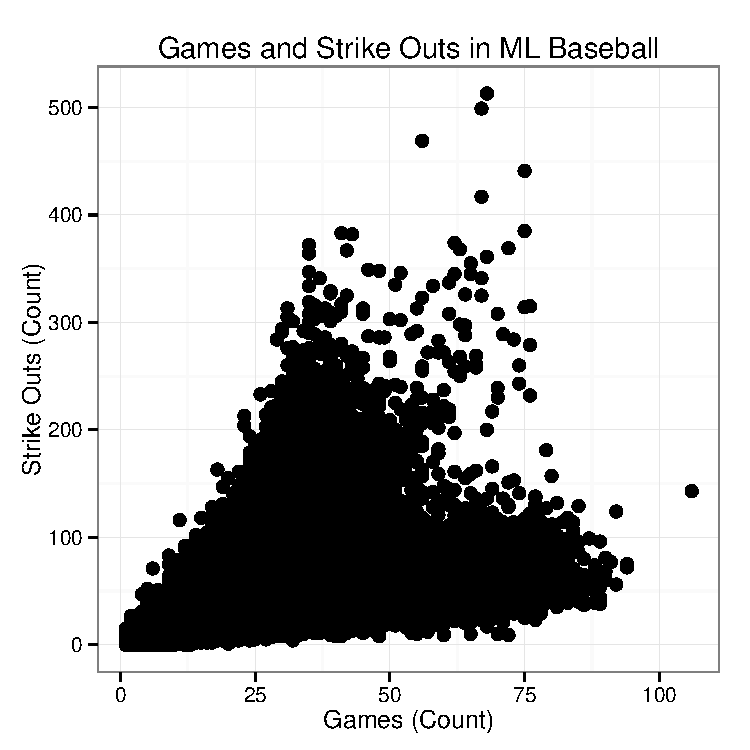
\includegraphics[keepaspectratio=TRUE,width=.31\textwidth]{./Body/BinnedScatter/figure/Overplotting.pdf}}
  \subfloat[Tukey-style open circles]{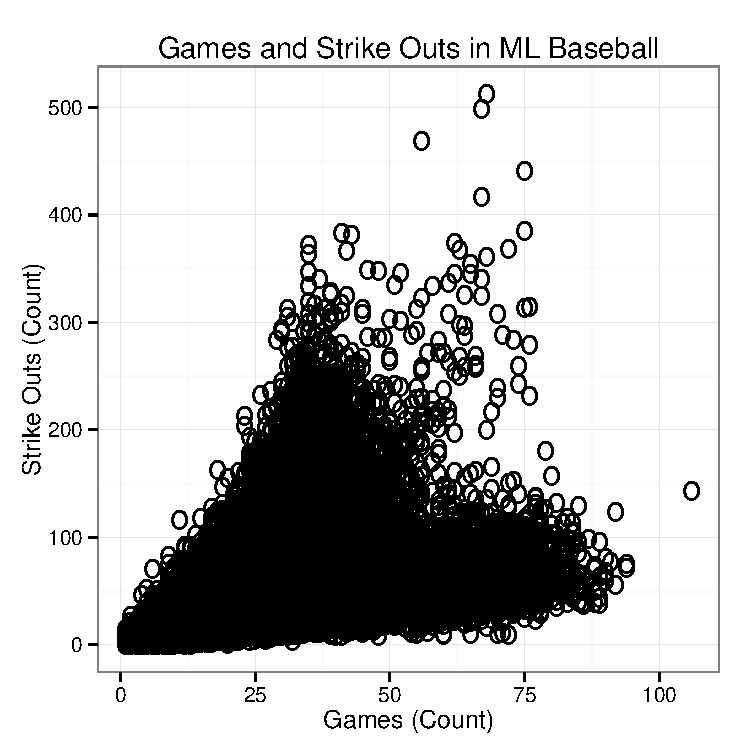
\includegraphics[keepaspectratio=TRUE,width=.31\textwidth]{./Body/BinnedScatter/figure/OverplottingCircles.pdf}} 
	\subfloat[Alpha blending]{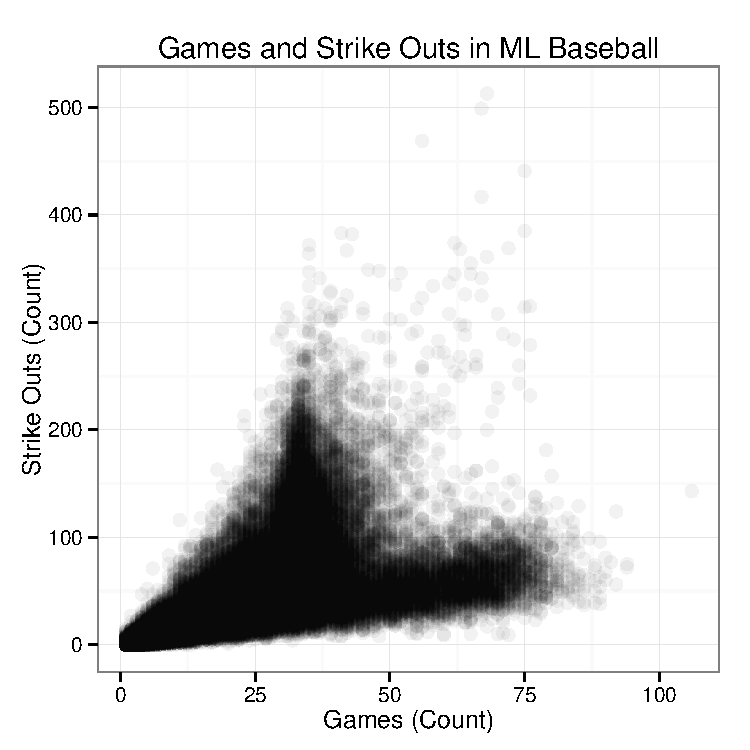
\includegraphics[keepaspectratio=TRUE,width=.31\textwidth]{./Body/BinnedScatter/figure/OverplottingAlpha.pdf}}
  
  \subfloat[Hexagonal binned scatterplot]{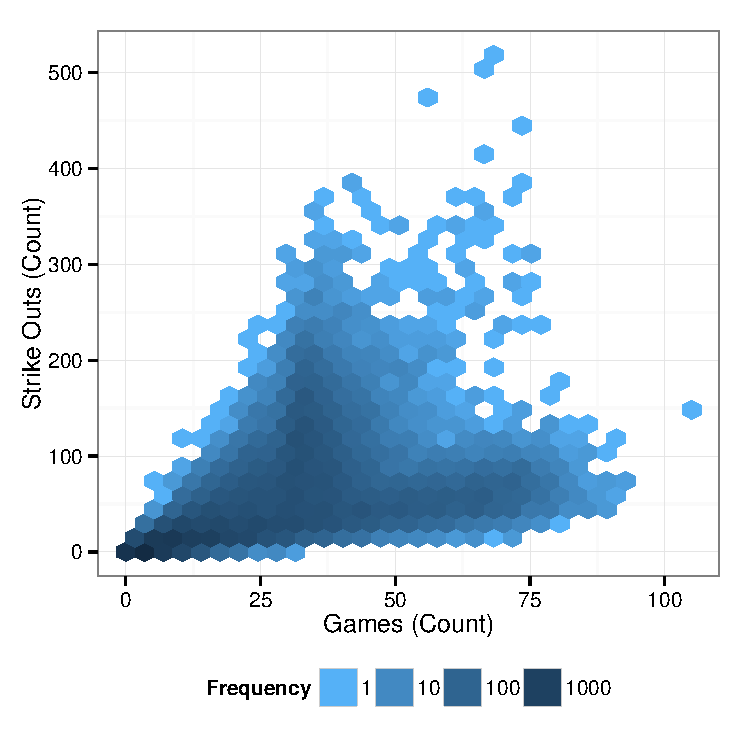
\includegraphics[keepaspectratio=TRUE,width=.48\textwidth]{./Body/BinnedScatter/figure/HexBinning.pdf}}
  \subfloat[Hexagonal binned bubble plot]{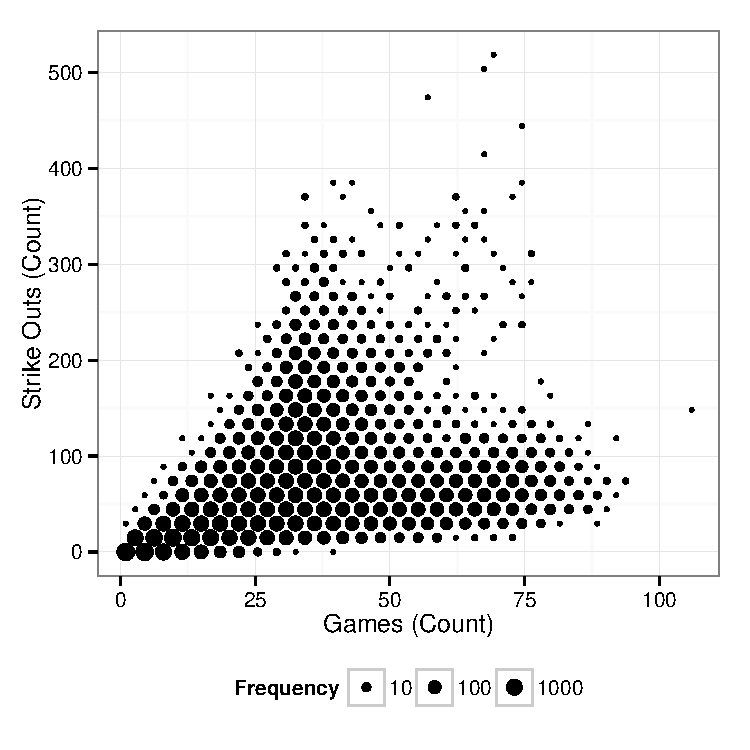
\includegraphics[keepaspectratio=TRUE,width=.48\textwidth]{./Body/BinnedScatter/figure/BinScatter.pdf}} 

	\caption{\label{fig:scatter-alpha} Scatterplots of Games versus Strikeouts in Major League Baseball, using different strategies of dealing with the issue of over-plotting:  (a) uses standard, opaque, filled circles, (b)  uses Tukey's recommended open circles, and (c) uses filled circles with alpha blending ($\alpha$=0.05). Plots (d) and (e) show hexagonal binning strategies with frequency mapped to color and area respectively}
\end{figure}

All of these methods fall short in the example.
As can be seen in Figure~\ref{fig:scatter-alpha}, strategy (a) is the least effective, as it provides information about the outliers and range of the data but cannot provide any point density information. Tukey's open circles (b) help to a degree, but are also prone to over-plotting  when the data set is very large. Alpha blending (c) highlights the structure, but minimizes the visual impact of outliers. The data set is large enough that neither alpha blending nor open circles are completely effective, and so we must pursue a different strategy which can provide better information about the relative density of points at a given location.

Other scatterplot adaptations have been introduced that avoid overplotting by manipulating the display of the points by distorting the locations or the scales. Generalized scatterplots \citep{Keim2010GenScatter} display all individual observations (including ties) but use distortion of the point locations by having points repel one another to avoid overlapping points.  An extension of generalized scatterplots uses clustering and local principal components to allow ellipsoid oriented distortion to display local correlation structure in the data \citep{Janetzko2013Ellipse}. Variable-binned scatterplots \citep{Hao2010visual} break the display into a non-uniform rectangular grid and resize the rows of cells according to density of points. This variable binning fragments the continuity of the axes into  segments on different scales and also does not deal with ties. Generalized and variable-binned scatterplots make fine data structure more visible and allow color to be reserved for a third variable instead of frequency; however, the distortion of the point locations and/or axes warp the visual display of the association between the two primary variables.

Another approach is to reduce the graphical complexity by plotting binned aggregations of the data, namely frequencies, as opposed to plotting every observation as an individual point. This has the additional advantage of reducing the size of the stored data necessary for the construction of the plot, as only the bin centers and the frequency of observations which correspond to that bin must be stored. Wickham argues for a ``bin-summarize-smooth'' procedure to be applied to the visualization of big data and he notes that simple summary functions, such as counts, scale  well with the size of data \citep{Wickham2013Bin}. Liu, Jiang and Heer employ the computational benefits of binning for their interactive big data visualization program, \textit{imMens} \citep{Liu2013imMens}.  

Methods commonly used to display binned variables include sunflower plots \citep{sunflowerplots}, kernel density smoothing of tonal variation and modified scatterplots \citep{martin-gold}.  Sunflower plots are scatterplots of binned data, where the symbol used for the bin increases in complexity in proportion to the number of points in that bin. Sunflower plots are particularly useful when the number of points in each bin remains reasonably small. Kernel density smoothing can be used to vary $\alpha$ or color according to a smoothed density, providing features similar to binned scatterplots or alpha blended scatterplots in a more smooth, continuous fashion. However, these estimates require careful parameter tuning, as over-smoothing may hide gaps in the data while simultaneously de-emphasizes outlying points.

Histograms are a simple example of a plot that can be built using binned aggregations of the data; in their case the bin locations and bin counts act as a set of sufficient statistics necessary to reconstruct the plot.  A natural extensions of histograms to higher dimensions is to form a tessellated grid on a two dimensional Cartesian plane using some other attribute, such as color or size (or 3D renderings, which we do not want to recommend at this point) to provide joint density information within each grid cell, known as a tile.  A {\it binned scatterplot} uses shading to provide frequency information, with tiles (rather than bars in a histogram) at the bin center, similar to a two-dimensional histogram viewed from above. A \textit{bubble plot} is a binned data plot that scales the size of a filled circle in proportion to frequency.  Bubble plots were first used by William Playfair \citep{playfair, playfair2}. 

Figure~\ref{fig:scatter-alpha} contains examples of a hexagonally binned scatterplot with frequency encoded as color (\ref{fig:scatter-alpha}d) and a bubble plot with frequency encoded as point size (\ref{fig:scatter-alpha}e). The hexagonal tiles and the modified scatterplot are more effective at displaying the shape of the joint density and preserving outliers than any of the scatterplots shown in Figure~\ref{fig:scatter-alpha} (a-c). The bubble plot is prone to suffer from the Hermann-grid illusion \citep{hermann:1870} especially for data binned on a grid; whereas the binned scatterplot will not on a tessellated grid. 

Only in the binned scatterplot and the bubble plot the inner structure of the data becomes apparent: the joint density consists two distinct ridges following two lines with very different slopes. The lower slope corresponds to the modern average strike out rate of pitchers of just under one strike-out per game. The other line has a slope of about four times that rate. This high rate is also associated with fewer games played. Closer investigation of other, related variables reveals that this high strike-out rate corresponds mainly to historic pitchers with much shorter seasons (in 1876 only 70 games were played in a season, as opposed to 162 in 2009), and qualitatively different balls and  bats.

For extremely large data sets, binned scatterplots are a more useful visualization of two-dimensional density information than the scatterplot, and are less computationally demanding, as not every single point in the data set has to be rendered separately. 

As with histograms, the width of bins (or the number of bins) is an important factor in the detail of the binned data and the resulting plot: if the bin width is too small in comparison to the amount of data available, there is little advantage to binning, but if the bin width is too large, interesting features of the joint distribution may be obscured by over-plotting. 


\section{Binning Algorithms}
\label{GenBinning}

Binning algorithms used in making distributional approximations can be traced back to Pearson's work with the binomial approximation to the normal, where he mentions the need to define an origin and binwidth for segmenting the normal distribution \citep{Pearson1895}. More recently Scott has presented discussion on the importance of binning specification in the creation of histograms to appropriately display one dimensional density approximations \citep{scott1979}. \citet{scott1992} extends to the properties of multivariate binning strategies.

Binning in dimensions $X$ and $Y$ provides us with a more condensed form of the data that ideally preserves both the joint distribution as well as the margins, while reducing the amount of information to a fraction of the original.  Binning is a two-step procedure: we first assign each observation $(x, y)$ to a bin center $(x^\ast,y^\ast)$, and in a second step we count the number of observations assigned to each unique bin center; resulting in  triples  of the form $(x^\ast, y^\ast, c)$, where $c$ is the number of all observations assigned to bin center $(x^\ast,y^\ast)$.

We will proceed with rectangular bins for simplicity, but other binning schemes, such as hexagonal bins \citep{scatterplots} are also common.  While hexagonal binning has been shown to have slightly better graphical properties \citep{scott1992}; rectangular bins are advantageous because bins in $x$ and $y$ are orthogonal to each other, thus we can present the one-dimensional case which will easily generalize to two or more dimensions.  We will however only consider binning in up to two dimensions, $X$ and $Y$. The algorithms we discuss are immediately applicable to higher dimension, but we do not feel that the paper would benefit from a more general discussion.

For the univariate case with observations, $x_i$ for $i \in \{1,\dots,n\}$, binning algorithms require a set of bin centers $x_j^\ast$ for $j \in \{1,\dots,J\}$ and a binning function $b_X(.) : x_i \rightarrow x^\ast_j$ that maps observations to  bin centers. 

\textit{Rectangular binning} accomplishes this by defining a sequence of $J$ adjacent intervals, $(\beta_{j-1},\beta_{j}]$ for $j \in \{1,\dots,J\}$, which span over the range of the data. Note that half open intervals are used such that any observation falling on a bin boundary is assigned to a unique interval. Values $x_i$ exactly equal to the lowest bin boundary $\beta_0$ are grouped into the first bin to close the leftmost bound. Each observation is then mapped to a bin center, $x_j^\ast$; the midpoint for the interval to which the observation belongs. 

This is expressed mathematically using the binning function $b_X(.) : x_i \rightarrow x^\ast_j$ is defined as 
%
\begin{eqnarray}\label{rectbin}
b_X(x_i) = \left\{\begin{array}{ll} 
  x^\ast_{1} &\text{ for all } x_i = \beta_{0} \\
  x^\ast_j & \text{ for all } x_i \in (\beta_{j-1} , \beta_j] 
  \end{array}\right.
\end{eqnarray}  
%

\textit{Standard rectangular binning} is a special cases of general rectangular binning that uses intervals of equal size for all bins; thus only the origin of the first bin, $\beta_0$, and a binwidth, $\omega_X$, need to be specified. Standard rectangular binning is necessarily used in the construction of all histograms;  the consistent binwidth makes the display of frequency proportional to density. Fixed width binning procedures are also highly computationally efficient \citep{Wickham2013Bin}. 

Note that this standard rectangular binning procedure utilizes intervals that are open to the left and closes the outer bound of the leftmost bin. These specifications are consistent with the binning procedure used in the \texttt{hist()} function for creating histograms in base \texttt{R} \citep{R}. These specifications were selected for this paper, but these choices are by no means consider universal for binning.  For example, the \texttt{ggplot2} package creates histograms with intervals open to the right and does not close the outer bound of the rightmost bin \citep{ggplot2}. 

\textit{Quantile binning} is another option that divides the range of the observations into bins each containing equal number of points. The $j^{th}$ bin intervals is $(Q_X((j-1)/J),Q_X((j)/J)]$, where $Q_X(p)$ is the the $p^{th}$ empirical quantile using the inverse empirical distribution function. Note that this binning approach is \textit{not} desirable for visualizing density patterns, as it effectively balances the frequency counts in all bins; it does however have desirable properties for creating discernible groups in visualization using discrete color palettes.
  
The bin boundaries and centers for each type of rectangular binning algorithm discussed above can be found in Table~\ref{tab:rectbinning}.
 
% \begin{table}[hbtp]
% \centering
% \begin{tabular}{lll} \hline
%  & Bin Boundaries & Bin Centers \\ 
%  \hline  
% General &  $ \{\beta_j \text{ }|\text{ } \beta_j > \beta_{j-1} \} $ & $\{x_j^\ast \text{ }|\text{ } x_j^\ast = (\beta_{j-1}+ \beta_j)/2 \}$ \\
% %-------------
% Standard \hspace{0.5cm} & $ \{\beta_j \text{ }|\text{ } \beta_j = \beta_{j-1} + \omega_X \} $\hspace{0.5cm} & $\{x_j^\ast \text{ }|\text{ } x_j^\ast = \beta_{j-1} + \omega_X/2 \}$ \\
% %-------------
% Quantile & $ \{\beta_j \text{ }|\text{ } \beta_j = Q_X(j/J) \} $  & $\{x_j^\ast \text{ }|\text{ } x_j^\ast = Q_X((j-0.5)/J) \}$ \\
% %-------------
% Random &  ---  & $\{x_j^\ast \text{ }|\text{ } x_j^\ast > x_{j-1}^\ast \}$  \\
% \hline
% \end{tabular}
% \caption{Rectangular and Random Binning Specifications}
% \label{tab:rectbinning}
% \end{table}
% %
% An alternative to the rectangular binning processes discussed above, is the random binning algorithm which utilizes a non-deterministic bin function $b^r_X(\cdot)$ which randomly assigns a value $x_i$ to a bin center, $x^\ast$, from a set of possible bins. In this paper, we will consider the simplest case of just two bins, so that without loss of generality we can assume that $x_i$ lies between bin centers $x^\ast_j$ and $x^\ast_{j+1}$. The bin function assigns $x_i$ to a bin center with a probability inversely proportional to the distance to that bin center; the closer a value is to a bin center, the higher the probability the value is assigned to that bin center. More formally,
% %
% \begin{eqnarray}\label{randbin1}
% b^r_X(x_i) = \left\{\begin{array}{ll} 
%   x^\ast_j & \text{ with probability } (x^\ast_{j+1} - x_i)/(x^\ast_{j+1} -x^\ast_{j}) \\
%   x^\ast_{j+1} &\text{ with probability }  (x_i - x^\ast_{j})/(x^\ast_{j+1} -x^\ast_{j})
%   \end{array}\right.
% \end{eqnarray}  
% %
% for $x_i \in [x^\ast_{j+1}, x^\ast_{j}]$.  This probability structure is inversely proportional to the distance from each bin center.  In Table~\ref{tab:rectbinning} we note that this random binning algorithm does not specify bin boundaries; only a sequence of bin centers.  This method is easily extensible to also map $x_i$ into more than two bins and can accommodate non-uniform distribution of bin centers.  
% 
% The deterministic standard binning algorithm is an example of a ``direct" binning algorithm, in which all points are assigned with weight one to the bin center. ``Linear" binning  \citep{martin-gold} is a \textit{computationally intensive} alternative to direct binning in which adjacent bins are assigned a weight depending on the distance from the point to that bin, where all weights sum to one.  With large data sets, the calculations required for linear binning become unwieldy, but the random binning algorithm can be considered an approximation to linear binning. Specifically, the expectation of the random binning algorithm is the same as for linear binning.
% 
% \subsection{Extension to Two Dimensional Binning}
% \label{TwoDimBin}
% 
% The standard and random binning algorithms are easily extendable to higher dimension. For the purposes of creating binned scatterplots we will specify extension to rectangular binning in two dimensions. In this case we wish to assign data pairs $(x_i, y_i)$ to bin centers of the form $(x_j^\ast,y_k^\ast)$, with $j \in \{1,\dots,J\}$ and $k \in \{1,\dots,K\}$, where $J$ and $K$ are the number of bins in the X and Y dimensions, respectively. The two ($j$,$k$) pairs that index the bin centers can be linearized to a single index such that $\ell = j + J(k-1)$; thus making $j$ the fast running index and $k$ the slow running index.  With this linearized index for all bins we now have a set of bin centers of the form $(x_\ell^\ast,y_\ell^\ast)$, with $\ell \in \{1,\dots,\mathscr{L}\}$, where $\mathscr{L}=J\cdot K$.
% 
% The standard rectangular binning function $b(.) : (x_i,y_i) \rightarrow (x^\ast_\ell,y^\ast_\ell)$ is defined as 
% %
% \begin{eqnarray}\label{standrecbin1}
% b(x_i,y_i) = (b_X(x_i),b_Y(y_i))
% \end{eqnarray}
% %
% where $b_X(x_i)$ and $b_Y(y_i)$ are the univariate standard binning algorithms for the X and Y dimensions respectively. The random rectangular binning function, $b^r(\cdot): (x_i,y_i) \rightarrow (x^\ast_\ell,y^\ast_\ell)$ is similarly be defined as
% %
% \begin{eqnarray}\label{randrecbin1}
% b^r(x_i,y_i) = (b^r_X(x_i),b^r_Y(y_i))
% \end{eqnarray}
% %
% where $b^r_X(x_i)$ and $b^r_Y(y_i)$ are univariate random binning algorithms for each dimension. Figure~\ref{fig:spatlossdemo2} provides an illustration of each binning process extended to a two dimensional situation.
% 
% % 
% % <<binningDemo,echo=F,include=F,cache=T>>=
% %       library(mvtnorm)
% %       set.seed(12)
% %       d <- rmvnorm(50, c(10, 25), matrix(c(50, 15, 15, 50), nrow=2))
% %       d <- data.frame(d)
% %       names(d) <- c("x", "y")
% %       d <- subset(d, (x>-20 & x<40 & y>0 & y<50),drop=TRUE)
% %       d.rand <- d
% %       dnew <- binStd(cbind(d-5, Freq=1), c(10, 10))
% %       dnew$x <- dnew$x+5
% %       dnew$y <- dnew$y+5
% %       d$bin <- dnew$x%in%c(5,15) & dnew$y==25
% %       d$a <- .33 + .66*d$bin
% %       d.orig <- d
% % 
% %       d$xbin <- NA
% %       d$ybin <- NA
% %       idx <- which(dnew$x%in%c(5, 15) & dnew$y==25)
% %       d$xbin[idx] <- dnew$x[idx]
% %       d$ybin[idx] <- 25
% % 
% % temp <- data.frame(   
% %           x=c( -10,   0,  10,  20,  30,  -10, -10, -10, -10), 
% %        xend=c( -10,   0,  10,  20,  30,   30,  30,  30,  30), 
% %           y=c( 10,   10,  10,  10,  10,   10,  20,  30,  40), 
% %        yend=c( 40,   40,  40,  40,  40,   10,  20,  30,  40), 
% %       group=c(  1,   2,   3,   4,   5,   6,   7,   8,   9))
% %       qplot(data=d[,], x=x, y=y, alpha=a,  geom="point", 
% %             xlim=c(-20, 40), ylim=c(0, 50)) +
% %         annotate("polygon", x=c(10, 10, 20, 20), y=c(20, 30, 30, 20), 
% %                  fill="blue", alpha=.25) +
% %         annotate("polygon", x=c(0, 0, 10, 10), y=c(20, 30, 30, 20), 
% %                  fill="green", alpha=.25) +
% %         scale_alpha(range=c(.5, 1), guide=FALSE) +
% %       #  scale_colour_identity(guide=FALSE) + 
% %       #  scale_shape(solid=T,guide=FALSE) +
% %         theme_bw() +
% %       #  annotate("point", x=rep(seq(-15, 35, 10),each=7), 
% %       #         y=rep(seq(-5, 55, 10), times=6), 
% %       #         shape='+', size=8, colour="gray90") + 
% %         geom_point(data=d[which(!is.na(d$xbin)),], 
% %                    aes(x=x, y=y, shape=factor(xbin), colour=factor(xbin)), 
% %                    size=I(3), aes.inherit=FALSE) + 
% %         scale_shape_manual(name="Bin", values=c("5"=16, "15"=15), 
% %                            labels=c("(5,25)", "(15, 25)"),guide=FALSE) +
% %         scale_colour_manual(values=c("5"="green", "15"="blue"), name="Bin", 
% %                             labels=c("(5,25)", "(15, 25)"),guide=FALSE)+
% %         annotate("segment", x=temp$x, y=temp$y, 
% %                  xend=temp$xend, yend=temp$yend, group=temp$group) + 
% %         ylim(c(10, 40)) + xlim(c(-10,30))
% %       ggsave("./figure/Binning-DataAndBin.pdf", width=5, height=5, units="in")
% %       
% %       d.orig$bin <- dnew$x==15 & dnew$y==25
% %       d.orig$a <- .33+.66*d.orig$bin
% %       d.orig$l <- "Data outside bin"
% %       d.orig$l[d.orig$bin] <- "Binned Data"
% %       d.orig$size <- 2
% %       d.orig$size[d.orig$bin] <- 3
% %       d.orig <- rbind(d.orig, data.frame(x=15, y=25, a=1, l="Visual Center", size=2,bin=TRUE),
% %         data.frame(x=mean(d.orig$x[d.orig$bin]), y=mean(d.orig$y[d.orig$bin]),                                                                                    
% %         l="Numerical Center", a=1, size=2, bin=TRUE))
% % #       ggplot(data=d.orig, aes(x=x, y=y, shape=l, size=l, colour=l)) + 
% % #         annotate("polygon", x=c(10, 10, 20, 20), y=c(20, 30, 30, 20), 
% % #                  fill="blue", alpha=.10) + 
% % #         geom_point() +
% % #         scale_shape_manual(name="", values=c("Data outside bin" = 16, 
% % #                                              "Binned Data" = 15, 
% % #                                              "Numerical Center" = 17, 
% % #                                              "Visual Center" = 18)) +
% % #         scale_colour_manual(name="", values=c("Data outside bin" = "grey60", 
% % #                                               "Binned Data" = "blue",
% % #                                               "Numerical Center" = "blue4", 
% % #                                               "Visual Center" = "blue4"))+
% % #         scale_size_manual(name="", values=c("Data outside bin" = 3, "Binned Data"=3,
% % #                                             "Numerical Center" = 5, 
% % #                                             "Visual Center" = 5))+
% % #         theme_bw() +
% % #         annotate("point", x=15, y=25, shape=18, size=5, colour="blue4") + 
% % #         annotate("point", x=d.orig$x[which(d.orig$l=="Numerical Center")], 
% % #                  y=d.orig$y[which(d.orig$l=="Numerical Center")], shape=17, size=5, 
% % #                  colour="blue4") +
% % # #        annotate("segment", x=temp$x, y=temp$y, xend=temp$xend, yend=temp$yend, group=temp$group) + 
% % # #         annotate("text", x=d$x[which(d$l=="Numerical Center")], 
% % # #                  y=d$y[which(d$l=="Numerical Center")], 
% % # #                  label=expression(paste('(', over(phantom(0),x)[i], ',', over(phantom(0),y)[i],')'))) +
% % #         scale_x_continuous(breaks=c(10, 15, 20), limits=c(8, 22), labels=c(expression(x^{"*"}-b[x]/2), expression(x^{"*"}), expression(x^{"*"}+b[x]/2)), name='') + 
% % #         scale_y_continuous(breaks=c(20, 25, 30), limits=c(18, 32), labels=c(expression(y^{"*"}-b[y]/2), expression(y^{"*"}), expression(y^{"*"}+b[y]/2)), name='')
% % #       ggsave("./figure/Binning-DataVisualNumericalCenter.pdf", width=5, height=4, units="in")
% % @
% % 
% % <<RandomBinDemo,echo=F,include=FALSE>>=
% % nl <- ncol(d.rand)
% % dnew <- d.rand
% % binning <- c(10, 10)
% % for(x in 1:(nl)){
% %   y <- d.rand[,x] - binning[x]/2
% % dnew[,x] <- binning[x]*(floor(y/binning[x]) + 
% %   sapply((y%%binning[x])/binning[x], function(p) rbinom(1, 1, p))) + binning[x]/2
% % }
% % temp <- data.frame(   
% %           x=c( -10,   0,  10,  20,  30,  -10, -10, -10, -10), 
% %        xend=c( -10,   0,  10,  20,  30,   30,  30,  30,  30), 
% %           y=c( 10,   10,  10,  10,  10,   10,  20,  30,  40), 
% %        yend=c( 40,   40,  40,  40,  40,   10,  20,  30,  40), 
% %       group=c(  1,   2,   3,   4,   5,   6,   7,   8,   9))
% % 
% % dnew$id <- interaction(dnew[,1:(nl)])
% % idx <- which(dnew$x%in%c(5, 15) & dnew$y==25)
% % d.rand$bin <- dnew$x%in%c(5, 15) & dnew$y==25
% % d.rand$a <- .33 + .66*d.rand$bin
% % d.rand$xbin <- NA
% % d.rand$ybin <- NA
% % d.rand$xbin[idx] <- dnew$x[idx]
% % d.rand$ybin[idx] <- 25
% % # res <- ddply(dnew, .(id), summarize, n=length(id), fsum=sum(Freq))
% % qplot(data=d.rand[,], x=x, y=y, alpha=a,  geom="point", xlim=c(-20, 40), ylim=c(0, 50)) +
% %   annotate("polygon", x=c(10, 10, 20, 20), y=c(20, 30, 30, 20), fill="blue", alpha=.25) +
% %   annotate("polygon", x=c(0, 0, 10, 10), y=c(20, 30, 30, 20), fill="green", alpha=.25) +
% %   scale_alpha(range=c(.5, 1), guide=FALSE) +
% %   scale_colour_identity(guide=FALSE) + 
% %   scale_shape(solid=T,guide=FALSE) +
% %   theme_bw() +
% % #  annotate("point", x=rep(seq(-15, 35, 10),each=7), 
% % #        y=rep(seq(-5, 55, 10), times=6), 
% % #         shape='+', size=8, colour="gray90") + 
% %   geom_point(data=d.rand[which(!is.na(d.rand$xbin)),], 
% %              aes(x=x, y=y, shape=factor(xbin), colour=factor(xbin)), size=I(3), aes.inherit=FALSE) + 
% %   scale_shape_manual(name="Bin", values=c("5"=16, "15"=15), labels=c("(5,25)", "(15, 25)"),guide=FALSE) +
% %   scale_colour_manual(values=c("5"="green", "15"="blue"), name="Bin", labels=c("(5,25)", "(15, 25)"),guide=FALSE)+
% %   annotate("segment", x=temp$x, y=temp$y, xend=temp$xend, yend=temp$yend, group=temp$group) + ylim(c(10, 40)) + xlim(c(-10,30))
% % ggsave("./figure/RandomBinningDataPoints2.pdf",width=5, height=5)
% % @
% % 
% % \begin{figure}[h]
% %   \centering
% %   \subfloat[Standard Binning]{\includegraphics[keepaspectratio=true, width=2.5in]{./figure/Binning-DataAndBin.pdf}}
% % %   \subfloat{\includegraphics[keepaspectratio=TRUE, width=2in]
% % %   {./figure/RandomBinningDataPoints1}}
% %   \subfloat[Random Binning]{\includegraphics[keepaspectratio=TRUE, width=2.5in]
% %   {./figure/RandomBinningDataPoints2.pdf}}
% %   \caption{Visualization of how data pairs are assigned to bins centered at (5, 25) and (15,25) under the two rectangular binning algorithms. Points in the standard algorithm are contained within the defined bin region, where points from the random algorithm may be assigned to any of the surrounding bin centers.}
% %   \label{fig:BinningTutorial}
% % \end{figure}
% 
% %--------------------------------------------------------------
% 
% \subsection{Binned Data Reduction}
% 
% The second stage of binning requires a frequency breakdown of the number of observations associated with each bin center, forming data triples, $(x^\ast, y^\ast, c)$, where $c$ is the number of all observations assigned to bin center $(x^\ast,y^\ast)$. Table~\ref{DataReductionExample} makes use of a small set of simulated data to show the progression from the original data (a), to the binned data (b), to the reduced binned data (c). The reduced binned data is sufficient for constructing the binned scatterplot. In cases of large data, binning greatly reduces the storage size for the information and the computation time needed to construct the plot.
% 
% <<DataReduction,echo=FALSE,eval=FALSE,results='asis'>>=
% n=12
% param1 = 1
% param2 = 1.6
% set.seed(52)
% x <- rbeta(n,param1, param2)*20-10
% y <- rbeta(n,param1, param2)*20-10
% # standard bin centers
% xcent <- rep(-5,n) ; xcent[x>0] <- 5
% ycent <- rep(-5,n) ; ycent[y>0] <- 5
% idx <- order(xcent,ycent)
% d <- data.frame(x,y,xcent,ycent)[idx,]
% dbin <- ddply(d, .(xcent,ycent), summarise,
%               c=length(x))
% dbin <- dbin[order(dbin$xcent,dbin$ycent),]
% 
% print(xtable(d[1:2], digits=c(0, 4, 4), caption=paste('Original Data\\newline', nrow(d), 'rows')), include.rownames=FALSE, table.placement="hbtp", floating=FALSE)
% 
% print(xtable(d[3:4], digits=c(0, 0, 0), caption=paste('Binned Data\\newline', nrow(d), 'rows')), include.rownames=FALSE, table.placement="hbtp", floating=FALSE)
% 
% print(xtable(dbin, digits=c(0, 0, 0, 0), caption=paste('Binned Data\\newline', nrow(dbin), 'rows'), align=c('X','X','X','c')), include.rownames=FALSE, table.placement="hbtp", floating=FALSE, tabular.environment="tabularx", width='.7\\textwidth')
% 
% @
% 
% \begin{table}[H]
% \begin{minipage}[t]{.33\textwidth}\centering\subfloat[Original Data, 12 rows]{
% \begin{tabular}{rr}\hline
%        $x$ &  $y$  \\ \hline
% -7.7325 & -9.6340 \\ 
%   -8.1176 & -1.4529 \\ 
%   -5.8996 & -3.2033 \\ 
%   -7.0375 & -5.5563 \\ 
%   -3.6354 & -3.9315 \\ 
%   -8.7639 & 0.9874 \\ 
%   -2.9781 & 8.6802 \\ 
%   0.8210 & -8.6118 \\ 
%   5.4477 & -8.4555 \\ 
%   4.6849 & -5.6620 \\ 
%   9.4785 & 1.1133 \\ 
%   1.7579 & 5.3759 \\  \hline
% \end{tabular}}
% \end{minipage}\hfil
% \begin{minipage}[t]{.33\textwidth}\centering\subfloat[Binned Data Centers, 12 rows]{
% \begin{tabularx}{.7\textwidth}{rr} \hline
%   $b_X(x)$ & \hspace{.4cm} $b_Y(y)$  \\ \hline
%   -5 & -5 \\ 
%   -5 & -5 \\ 
%   -5 & -5 \\ 
%   -5 & -5 \\ 
%   -5 & -5 \\ 
%   -5 & 5 \\ 
%   -5 & 5 \\ 
%   5 & -5 \\ 
%   5 & -5 \\ 
%   5 & -5 \\ 
%   5 & 5 \\ 
%   5 & 5 \\  \hline
% \end{tabularx}}
% \end{minipage}\hfil
% \begin{minipage}[t]{.33\textwidth}\centering\subfloat[Reduced Binned Data, 4 rows]{
% \begin{tabularx}{.7\textwidth}{rrr}\hline
%  \hspace{.2cm} $x^\ast$   &   \hspace{.2cm} $y^\ast$ & \hspace{.4cm}c \\ \hline
% -5 & -5 & 5 \\ 
%   -5 & 5 & 2 \\ 
%   5 & -5 & 3 \\ 
%   5 & 5 & 2 \\  \hline
% \end{tabularx}}
% \end{minipage}
% \caption{\label{DataReductionExample}Original, Binned and Reduced Binned Data Tables, with data storage sizes.  Binned using standard rectangular approach with origin $(\beta_{0,x},\beta_{0,y})$ = (-10,-10) and binwidths $\omega_x = \omega_y = 10$. }
% \end{table}
% 
% Note that numerical attributes other than frequency of the binned data may also be recorded during binning, however only frequency is required to construct a binned scatterplot. Data reduction comes at the expense of spatial information of any of the individual points. After aggregation the original spatial locations cannot be recovered. The loss of information incurred from binning will be explored in following sections. 
% 
% % \subsection{Standard Rectangular Binning Algorithm (old - to be removed)}
% % \hh{XXX Speed this discussion up a bit - you don't need to lay out what you will do in this section, just do it.}
% % 
% % \hh{Define what $X$ is, what is $x_i$}
% % 
% % \hh{Use only $1 \le j \le N_X$  or $j \in \{1, ..., N_X\}$. }
% % 
% % \hh{I am still not sure how bin centers are defined in the end. XXX}
% % 
% % \hh{why does it say binwidths? Do you want to imply that the bins have potentially different widths? Clarify that!}
% % 
% % \ktm{  We define the process that allocates observed values, $x_i$ for $i \in \{1, ..., n\}$, to equal sized bins in a deterministic manner as a standard binning algorithm. The bins are controlled by two parameters: the center of the first bin, $x^\ast_1$ and the binwidth, $\omega_X$. This leads to bin centers $ x_j^\ast =  x_1^\ast + (j-1)\omega_X \text{ for } j \in \{1, ..., N_X\} $,  where $N_X$ is the overall number of bins.  }
% % 
% % 
% % Mathematically, the standard binning algorithm corresponds to a function $b_X(.)$ that assigns to a value $x_i$ the closest bin center $x^\ast_j$ for some bin $j \in \{1, ..., N_X\}$, i.e. the binning function   $b_X(.) : x_i \rightarrow x^\ast_j$ is defined as 
% % % \begin{center}
% % % $x^\ast_i = b_X(x_i) = x_{(1)}^\ast + \omega_X \cdot \left\lfloor (x_i-x_{(1)})/\omega_x \right\rfloor$ \hspace{.5cm} $\forall x_i < x_{(n)}$, and \\ 
% % % \vspace{.03}
% % % $x^\ast_i = b_X(x_i) = x_{(n)} - \omega_x/2$ \hspace{.5cm} $\forall x_i = x_{(n)}$
% % % \end{center}
% % \begin{eqnarray}\label{standbin}
% % b_X(x_i) =  x_{1}^\ast + \omega_X \cdot \left\lfloor (x_i-x_{1}^\ast)/\omega_x + 1/2 \right\rfloor
% % \end{eqnarray}
% % 
% % where $x_1^\ast$ is the center of the first bin and $\lfloor . \rfloor$ denotes the floor function, $\lfloor x \rfloor$ is the largest integer value smaller than $x$.  
% % \ktm{ This is equivalent to treating the $j^{th}$ bin as a half-open interval that contains all observations $x_i \in [x_j^\ast - \omega_X /2 , x_j^\ast + \omega_X /2  ) $. After all observations have been allocated to bins, the bin count, $c_j$, is joined with the bin center to form the tuple $(x^\ast_1, c_j)$ }
% % %\hh{something went wrong with the next sentence}
% % %An intuitive understanding of the formula is developed by noting $\left\lfloor (x_i-x_{1}^\ast)/\omega_x + 1/2 \right\rfloor$ represents the number of bin boundaries lie between $x_{1}^\ast$ and $x_i$.  Thus, the binning function is finding the location of the bin center for $x_i$ by adding the distance between $x_{1}^\ast$ and the center for $x_i$ to the known first bin center $x_{1}^\ast$.
% % 
% % \ktm{ A special case of standard binning divides the data range into $N_X$ equal sized bins.  This leads to the bin width, $\omega_X = (x_{(n)} - x_{(1)})/N_X$, where $x_{(1)}$ and $x_{(n)}$ denote the observed minimum and the maximum of $X$, respectively. The first bin would then be centered at $x_{(1)} + \omega_X/2$. }
% % 
% % 
% % 
% % %Note that the binning function above amounts to dividing up the range of data by a specified number of bins of equal width. A more flexible binning algorithm may be achieved if we allow the specification of the first bin center and bin width instead of the number of bins. This strategy would still fit into the framework of assigning values to the closest bin center. 
% % 
% % \subsection{Random Binning Algorithm (old-to be removed)}
% % 
% % An alternative to the standard binning processes discussed above, is the random binning algorithm which results in statistically nice properties. A random binning algorithm utilizes a non-deterministic bin function $b^r_X(\cdot)$ which randomly assigns a value $x_i$ to a bin center, $x^\ast$, from a set of possible bins. In this paper, we will consider the simplest case of just two bins, so that without loss of generality we can assume that $x_i$ lies between bin centers $x^\ast_j$ and $x^\ast_{j+1}$. The bin function assigns $x_i$ to a bin center with a probability depending on the distance to that bin center; the closer a value is to a bin center, the higher the probability the value is assigned to that bin center. More formally,
% % %
% % \begin{eqnarray}\label{randbin}
% % b^r_X(x_i) = \left\{\begin{array}{ll} 
% %   x^\ast_j & \text{ with probability } p = {(x^\ast_{j+1} - x_i)}/\omega_X \\
% %   x^\ast_{j+1} &\text{ with probability } 1-p = {(x_i - x^\ast_{j})}/\omega_X
% %   \end{array}\right.
% % \end{eqnarray}
% % 
% % % In this manner, the probability of assigning point $x$ to bin $x^\ast_j$ is inversely proportional to the distance between the bin center of bin $x^\ast_j$ and $x$, that is, the closer $x$ is to a bin center, the higher the probability that $x$ will be assigned to that bin. 
% % This method is easily extensible to also map $x_i$ into more than two bins and can accommodate non-uniform bin sizes, unlike the standard algorithm. 
% % 
% % %To take up the previous number example again, under random binning the values 1.35, 1.55, and 2.35 are assigned to bin centers $\{1, 2, 3\}$ non-deterministic. 
% % %Value 1.35 has a 35\% probability to be assigned to bin center 2, and accordingly is assigned to bin center 1 with probability 65\%. 
% % %1.55 is closer to the boundary between bin centers and has therefore a 45\% or 55\% chance to be assigned to bin centers 1 or 2, respectively.
% % 
% % %Figure~\ref{fig:BinningTutorial} illustrates one possible outcome of the random binning process.
% % 
% % The deterministic standard binning algorithm is an example of a ``direct" binning algorithm, in which all points are assigned with weight one to the nearest bin. ``Linear" binning  \citep{martin-gold} is a \textit{computationally intensive} alternative to direct binning  in which adjacent bins are assigned a weight  depending on the distance from the point to that bin, where all weights sum to one.  With large data sets, the calculations required for linear binning become unwieldy, but the random binning algorithm can be considered an approximation to linear binning. Specifically, the expectation of the random binning algorithm is the same as for linear binning.
% % %However, linear binning requires evaluation of this expectation, whereas the random binning algorithm presented here uses a random sample from the underlying distribution, which is much more computationally tractable.
% % In the next section, we examine the loss of visual and numerical information due to binning.
% % % linear binning in Gold book - random algorithm as a less computational method of linear binning
% % 
% % \subsection{Extensions to Rectangular Binning (old-to be removed)}
% % 
% % The standard and random binning algorithms are easily extendable to higher dimension. For the purposes of creating binned scatterplots we will specify extension to rectangular binning in two dimensions. In this case we wish to assign data pairs $(x_i, y_i)$ to bin centers of the form $(x_j^\ast,y_j^\ast)$, with $1 \le j \le N_X \cdot N_Y =J$, where $J$ total number of indexed bins \sout{in $\mathbb{R}^2$} \hh{XXX J is an integer number, definitely not a real-valued vector}. \ktm{The wording here was not clear. J does not exist in $\mathbb{R}^2$, but it is being used to index 2d bins that exist in that plane.} The standard rectangular binning function $b(.) : (x_i,y_i) \rightarrow (x^\ast_j,y^\ast_j)$ is defined as 
% % %
% % \begin{eqnarray}\label{standrecbin}
% % b(x_i,y_i) = (b_X(x_i),b_Y(y_i))
% % \end{eqnarray}
% % %
% % where $b_X(x_i)$ and $b_Y(y_i)$ are the univariate standard binning algorithms for the X and Y dimensions respectively. The random rectangular binning function, $b^r(\cdot): (x_i,y_i) \rightarrow (x^\ast_j,y^\ast_j)$ can similarly be defined as
% % %
% % \begin{eqnarray}\label{randrecbin}
% % b^r(x_i,y_i) = (b^r_X(x_i),b^r_Y(y_i))
% % \end{eqnarray}
% % %
% % where $b^r_X(x_i)$ and $b^r_Y(y_i)$ are univariate random binning algorithms for each dimension. Figure~\ref{fig:BinningTutorial} provides an illustration of each binning process extended to a two dimensional situation.
% % 
% % \hh{The relationship between value pair $(x_i, y_i)$ and bin center $(x^\ast_j,y^\ast_j)$ needs to be discussed further - because it is not the same as for the univariate situation. $J$ is defined, as above as a multiple of $N_X$ and $N_Y$, this needs to be properly adjusted in the binning algorithm. It will be some linear relationship of the form $j_X\cdot N_X + j_Y$. }  \ktm{ I am having trouble trying to reconcile the indexing of bins in 2 dimensions.  If we use an pair of indices it makes the extension of binning to 2 dimensions easy; but it makes the notation messier and loss functions more difficult to define. }
% % 
% % 
% % 
% % \subsection{Quantile Binning Algorithm (old - to be removed)}
% % 
% % We could also consider a empirical quantile based binning algorithm where bin widths are adjusted such that each bin contains an equal proportion of the observed values. This is a fundamentally different approach than the standard and random binning algorithms defined previously where the goal was to display approximate density. This binning will not be considered for binning the data pairs directly, but instead for further binning the initial bin counts for the purposes of rendering colors on a discrete color palette.
% % 
% % Suppose that we have values $c_j$ for $j \in \{1,2,...J\}$ that we wish to divide into quantile based bins. Defining the number of quantile based bins, $K$, results in a set of possible quantile bin centers. \hh{shouldn't you go back to the same notation as before? $N_X$, not $J$?  what are the $c_j$ bin centers? before they were $c_j^\ast$.} \ktm{I consciously decided to define quantile binning in a way consistent with how it will be used later in the paper for discretizing the color palettes for the $c_j$ counts. } It follows that the bin boundaries are $Q_{k/K}$ for $k \in \{1,\dots,K\}$, where $Q_p$ is the the $p^{th}$ empirical quantile of value using the inverse empirical distribution function. \ktm{Note this is the quantile function as defined in R; find related literature source.} \hh{which function exactly? There are multiple.} The bin centers are defined as the midpoint of each consecutive pair of bin boundaries $\{c^\ast_k = (Q_{k-1/K} + Q_{k/K})/2  \text{ for } k=0,\dots,K \}$. The quantile binning function $b^q_C(\cdot) : (c_j) \rightarrow c^\ast_k$ is defined as 
% % %
% % \begin{eqnarray}\label{quantbin}
% % b^q_C(c_j) = (Q_{k-1/K} + Q_{k/K})/2 \text{ where } Q_{k-1/K} < c_j \le Q_{k/K}.
% % \end{eqnarray}
% % %
% % The two dimensional analog for quantile binning is not explored, as this binning strategy will be used in strictly the univariate setting for this manuscript.
% 
% %--------------------------------------------------------------
% 
% \section{Loss due to Binning}
% \label{LossIntro}
% 
% The problems with large data in scatterplots arise from overplotting, which is a form of implicit data aggregation. In order to keep track of overplotting, we switch to a weighted form of displays and explicitly keep track of overplotting. The reduced binned data carries the sufficient information necessary to render the binned scatterplot. Making the data aggregation explicit allows us to calculate the loss we experience.
% 
% Using a minimal bin width, a binned scatterplot is comparable to a standard scatter plot, with bins shaded in a binary manner, as each unique observed value is located in a different bin. Alpha blending as used in Figure~\ref{fig:scatter-alpha}c extends the binary shading of a standard scatterplot to an implicit shading according to frequency. The shading is implicit because the range of frequency information is not scaled to the range of shading values, so that maximum color saturation is usually reached well before the maximum frequency, truncating the perceivable frequency information. By explicitly shading bins according to frequency, more information is preserved than in a traditional scatter plot, as the frequency domain provides visual weight to tiles which represent more points. This generalization allows us to describe the plots in Figure~\ref{fig:scatter-alpha}d and e under the same framework as plots a-c. 
% 
% By additionally increasing the bin width, we provide increasingly higher-level summaries of the data by smoothing over local structures. Using a small number of large bins may mask the real signal in the data, while an extremely large number of small bins may not sufficiently smooth over {\it noise} inherent in any real data set. Figure~\ref{binning} gives an overview of a data set and binned representations using different numbers of bins, demonstrating the loss of information with increasing bin size. 
% 
% \begin{figure}[hbtp]
% <<binning_setup, echo=FALSE,fig.width=2, fig.height=2, out.width='\\linewidth'>>=
% set.seed(46)
% x <- round(rnorm(200), digits=2)
% y <- round(rnorm(200), digits=2)
% X <- data.frame(x,y)
% @
% \begin{minipage}{.35\linewidth}
% <<first, echo=FALSE, out.width='\\linewidth',fig.width=4, fig.height=4>>=
% qplot(x,y, asp=1, main='Unbinned Data')+theme_bw()
% @
% \end{minipage}
% \hfil\begin{minipage}{.645\linewidth}
% \begin{minipage}{.495\linewidth}
% <<bin001, echo=FALSE, out.width='\\linewidth',fig.width=4, fig.height=5>>=
% binwidth=0.1
% binout1 <- RectBin2d(x,y,-binwidth/2,-binwidth/2,binwidth,binwidth,type="standard")[[1]]
% qplot(x,y, asp=1, geom="blank") +
%   geom_tile(binwidth=binwidth, aes(x=binxs, y=binys, fill=binfreq), data=binout1) +
%   ggtitle(sprintf("binwidth = %.2f", binwidth)) +
%   geom_vline(aes(xintercept=seq(min(binout1$binxs)-binwidth, max(binout1$binxs),
%                                 by=binwidth)+binwidth/2), colour="grey90") + 
%   geom_hline(aes(yintercept=seq(min(binout1$binys)-binwidth, max(binout1$binys),
%                                 by=binwidth)+binwidth/2), colour="grey90") +
%   theme_bw() + theme(panel.grid.major= element_blank(),
%                      panel.grid.minor= element_blank(), legend.position="bottom") +
%   scale_fill_gradient(low="#56B1F7", high="#132B43", guide="legend",
%                       trans="log", breaks=c(1, 2, 5, 10, 20))
% 
% @
% \end{minipage}\hfil
% \begin{minipage}{.495\linewidth}
% <<bin025, echo=FALSE, out.width='\\linewidth',fig.width=4, fig.height=5>>=
% binwidth=0.25
% binout1 <- RectBin2d(x,y,-binwidth/2,-binwidth/2,binwidth,binwidth,type="standard")[[1]]
% qplot(x,y, asp=1, geom="blank") +
%   geom_tile(binwidth=binwidth, aes(x=binxs, y=binys, fill=binfreq), data=binout1) +
%   ggtitle(sprintf("binwidth = %.2f", binwidth)) +
%   geom_vline(aes(xintercept=seq(min(binout1$binxs)-binwidth, max(binout1$binxs),
%                                 by=binwidth)+binwidth/2), colour="grey90") + 
%   geom_hline(aes(yintercept=seq(min(binout1$binys)-binwidth, max(binout1$binys),
%                                 by=binwidth)+binwidth/2), colour="grey90") +
%   theme_bw() + theme(panel.grid.major= element_blank(),
%                      panel.grid.minor= element_blank(), legend.position="bottom") +
%   scale_fill_gradient(low="#56B1F7", high="#132B43", guide="legend",
%                       trans="log", breaks=c(1, 2, 5, 10, 20))
% @
% \end{minipage}\\
% \hfil\begin{minipage}{.495\linewidth}
% <<bin05, echo=FALSE, out.width='\\linewidth',fig.width=4, fig.height=5>>=
% binwidth=0.5
% binout1 <- RectBin2d(x,y,-binwidth/2,-binwidth/2,binwidth,binwidth,type="standard")[[1]]
% qplot(x,y, asp=1, geom="blank") +
%   geom_tile(binwidth=binwidth, aes(x=binxs, y=binys, fill=binfreq), data=binout1) +
%   ggtitle(sprintf("binwidth = %.2f", binwidth)) +
%   geom_vline(aes(xintercept=seq(min(binout1$binxs)-binwidth, max(binout1$binxs),
%                                 by=binwidth)+binwidth/2), colour="grey90") + 
%   geom_hline(aes(yintercept=seq(min(binout1$binys)-binwidth, max(binout1$binys),
%                                 by=binwidth)+binwidth/2), colour="grey90") +
%   theme_bw() + theme(panel.grid.major= element_blank(),
%                      panel.grid.minor= element_blank(), legend.position="bottom") +
%   scale_fill_gradient(low="#56B1F7", high="#132B43", guide="legend",
%                       trans="log", breaks=c(1, 2, 5, 10, 20))
% @
% \end{minipage}\hfil
% \begin{minipage}{.495\linewidth}
% <<bin1, echo=FALSE, out.width='\\linewidth',fig.width=4, fig.height=5>>=
% binwidth=1
% binout1 <- RectBin2d(x,y,-binwidth/2,-binwidth/2,binwidth,binwidth,type="standard")[[1]]
% qplot(x,y, asp=1, geom="blank") +
%   geom_tile(binwidth=binwidth, aes(x=binxs, y=binys, fill=binfreq), data=binout1) +
%   ggtitle(sprintf("binwidth = %.2f", binwidth)) +
%   geom_vline(aes(xintercept=seq(min(binout1$binxs)-binwidth, max(binout1$binxs),
%                                 by=binwidth)+binwidth/2), colour="grey90") + 
%   geom_hline(aes(yintercept=seq(min(binout1$binys)-binwidth, max(binout1$binys),
%                                 by=binwidth)+binwidth/2), colour="grey90") +
%   theme_bw() + theme(panel.grid.major= element_blank(),
%                      panel.grid.minor= element_blank(), legend.position="bottom") +
%   scale_fill_gradient(low="#56B1F7", high="#132B43", guide="legend",
%                       trans="log", breaks=c(1, 2, 5, 10, 20))
% @
% \end{minipage}
% \end{minipage}
% \caption{\label{binning}Series of scatterplots showing the original data (scatterplot, left), and versions of the binned data for different bin widths. The visual loss from binning at 0.1 is minimal, while a bin width of 1 gives a rough approximation.}
% \end{figure}
% 
% In the first set of binned data, the bins and the points on the scatterplot are nearly identical, but the scatterplot contains information about overlapping points. The second and third sets of binned data, with bin width equal to 0.25 and 0.50 respectively, show higher-level summaries of the data but which may also provide more visually accessible information about the shape of the two-dimensional density between $x$ and $y$. The fourth set of binned data with bin width equal to 1.0 is nearly unrecognizable, because the bins are large enough that they provide very little additional information. 
% 
% Loss of information occurs during the binning and rendering process. For the remainder of the paper we will assume that we are using colors in binned scatterplots to represent frequencies.  We distinguish two sources of loss in the construction of a binned scatterplot:
% 
% 
% \begin{itemize}
% \item {\it Spatial Loss}, $L^\text{S}$, occurs when points $(x_i, y_i)$ for observations $i \in \{1,\dots,n\}$ in the data set are reduced to a set of tiles centered at $(x_\ell^\ast, y_\ell^\ast)$ for bins $\ell \in \{1,\dots,\mathscr{L}\}$. By displaying frequency information using shaded tiles instead of individual points there is a loss of information about the exact location of the points. %\hh{XXX the frequency information is not what causes the loss}
% 
% \item {\it Frequency Loss}, $L^\text{F}$, occurs when bin counts, $c_\ell \in \{1,\dots,\mathscr{L}\}$ are not mapped to a continuous shading scale. While shade can be \textit{rendered} continuously in HSV color space, thus representing frequency exactly, a human reader can not \textit{extract} this information at the same precision due to limitations of  human cognition.  %A discrete color scale may be used to aid the ability to read a binned scatterplot, however this is effectively 
% In order to model these limitations we 
% introduce a second stage of binning by using a discrete color scale for displaying binned frequencies, $b_C(c_\ell)$, $\ell \in \{1,\dots,\mathscr{L}\}$. %This loss in precision is then quantified as {\it Frequency loss}. %, thus losing precision in the display of the true frequencies.
% 
% \end{itemize}
% 
% 
% %\hh{XXX ok, I don't quite agree with the description of frequency loss here. (a) the rendering on a continuous color scheme IS precise. but on a cognitive level we are not able to read the rendered values at the same precision. This effectively intorduces a second stage of binning ... then we are on the same page again.} \ktm{Is this new description any better?}
% 
% 
% Note that even though the losses from creating a binned scatterplot may turn out to be substantial there a huge gain with respect to the original scatterplot, where information can be masked in large data situations due to over-plotting of points. The idea of loss from one-dimensional binning was explored by Scott using mean squared error as the loss function to be optimized by the choice of the number of bins in  the construction of histograms \citep{scott1979}. He later extended this discussion to two-dimensional binning, where he compared the mean squared error loss for hexagonal, rectangular and triangular binning; finding that hexagonal and rectangular binning performed similarly, both far superior to triangular binning \citep{scott1992}. We will take a similar approach to quantifying loss resulting from the binning algorithms detailed in Section~\ref{GenBinning} above. 
% 
% \subsection{Spatial Loss}
% \label{SpatialLoss}
% 
% When the individual points of a scatterplot are collapsed to bin centers to be displayed as tiles in a binned scatterplot there is a loss of the location information.  This can be expressed as the Euclidean distance between points and the visual center of the tiles (i.e.\ the bin centers). Note that other distance metrics could be used, but the Euclidean distance has a desirable interpretability in $\mathbb{R}^2$. The \textit{total spatial loss}, $L^S$, is defined as 
% \begin{eqnarray}\label{totspatloss}
% L^S = \sum_{i=1}^{n} L_i^S = \sum_{i=1}^{n} \sqrt{ \left(x_i-b_X(x_i)\right)^2 + \left(y_i-b_Y(y_i)\right)^2 }
% \end{eqnarray} 
% %
% where $L_i^S$ is the loss in the  $i$th observation. 
% %
% Figure~\ref{fig:spatlossdemo2} visually displays the spatial loss for the data from  Table~\ref{DataReductionExample} as a result of standard rectangular binning. Observations $(x_i,y_i)$ and bin centers $\left(x_\ell^\ast,y_\ell^\ast\right)$ are displayed as black points and gray crosses, respectively. The length of line segments connecting these represent $L^S_i$, the spatial loss for each observation; thus, the combined length of all segments represents the total spatial loss, $L^S$.  
% 
% <<spatlossdemo2,echo=F,include=T,eval=T,fig.width=12, fig.height=6, out.width='1\\linewidth', fig.pos='h',fig.align='center',tidy=F, cache=TRUE, fig.show='hold',fig.cap="Visualization of spatial loss for same data using standard, random and post-processed random binning algorithms.  Note that the total spatial loss for the standard algorithm is smaller than by random binning. The net spatial loss for the original random binned data is the total spatial loss of the post-processed assignment." >>= 
% n=12
% param1 = 1
% param2 = 1.6
% set.seed(52)
% x <- rbeta(n,param1, param2)*20-10
% y <- rbeta(n,param1, param2)*20-10
% # standard bin centers
% xcent <- rep(-5,n) ; xcent[x>0] <- 5
% ycent <- rep(-5,n) ; ycent[y>0] <- 5
% # standard bin gridlines
% temp <- data.frame(   
%   x=c( -10,   0,  10, -10, -10, -10), 
%   xend=c( -10,   0,  10,  10, 10, 10), 
%   y=c( -10, -10 , -10 , -10, 0 , 10), 
%   yend=c(10, 10 , 10, -10, 0, 10 ))
% 
% p1 <- qplot(xcent, ycent, geom="point", size=I(5), shape=I(3), color=I("gray")) +
%       geom_segment(aes(x = x, y = y, xend = xend, yend = yend), data=temp) + 
%       geom_segment(aes(x = x, y = y, xend = xcent, yend = ycent)) + 
%       geom_point(aes(x=x,y=y), size=I(3))+ 
%       theme_bw() + xlab("") + ylab("") +
%       ggtitle("Standard Binning") +
%       theme(panel.grid.major= element_blank(),panel.grid.minor= element_blank(),
%             legend.position="none",plot.margin = unit(c(0,1,0, 1),"cm"),
%             aspect.ratio=1)
% 
% # random bin centers
% set.seed(14)
% rxcent <- RandRectBin1d(x, -10, 10)
% rycent <- RandRectBin1d(y, -10, 10)
% # point 1 and 11 are special 
% linecolor <- rep("blue", 12)
% linecolor[c(1,11)] <- "red"
% 
% p2 <- qplot(xcent, ycent, geom="point", size=I(5), shape=I(3), color=I("gray")) +
%   geom_segment(aes(x = x, y = y, xend = xend, yend = yend), data=temp) + 
%   geom_segment(aes(x = x, y = y, xend = rxcent, yend = rycent, color=linecolor)) + 
%   scale_colour_manual(values = c("darkblue","red"))+
%   geom_point(aes(x=x,y=y), size=I(3))+ 
%   theme_bw() + xlab("") + ylab("") +
%   ggtitle("Random Binning") +
%   theme(panel.grid.major= element_blank(),panel.grid.minor= element_blank(),
%         legend.position="none",plot.margin = unit(c(0,1,0, 1),"cm"),
%             aspect.ratio=1)
% 
% # post process random bin centers to visually 
% # equivalent allocation with minimum spatial loss
% rxcentpost <- rxcent
% rycentpost <- rycent
% rxcentpost[1] <- rxcent[11]
% rycentpost[1] <- rycent[11]
% rxcentpost[11] <- rxcent[1]
% rycentpost[11] <- rycent[1]
% # point 1 and 11 are special 
% linecolor <- rep("blue", 12)
% linecolor[c(1,11)] <- "red"
% 
% p3 <- qplot(xcent, ycent, geom="point", size=I(5), shape=I(3), color=I("gray")) +
%   geom_segment(aes(x = x, y = y, xend = xend, yend = yend), data=temp) + 
%   geom_segment(aes(x = x, y = y, xend = rxcentpost, yend = rycentpost, color=linecolor)) + 
%   scale_colour_manual(values = c("darkblue","red"))+
%   geom_point(aes(x=x,y=y), size=I(3))+ 
%   theme_bw() + xlab("") + ylab("") +
%   ggtitle("Post-Processed Random Binning") +
%   theme(panel.grid.major= element_blank(),panel.grid.minor= element_blank(),
%         legend.position="none",plot.margin = unit(c(0,1,0, 1),"cm"),
%             aspect.ratio=1)
% 
% allbin <- data.frame(type=rep(c("Standard","Random","Post-Processed Random"),each=n),
%                      binxs = c(xcent,rxcent,rxcentpost), 
%                      binys = c(ycent,rycent,rycentpost))
% allbinfreq <- ddply(allbin, .(type,binxs,binys),summarise,
%                      freq = length(binxs))
% 
% p4 <- qplot(xcent, ycent, geom="point", size=I(5), shape=I(3), color=I("gray")) +
%   geom_tile(aes(x=binxs, y=binys, fill=freq),data=subset(allbinfreq,type=="Standard")) + 
%   scale_fill_gradient(low="#56B1F7", high="#132B43", guide="legend") + 
%   theme_bw() + xlab("") + ylab("")  +
%   theme(panel.grid.major= element_blank(),panel.grid.minor= element_blank(),
%         plot.margin = unit(c(0,1,0, 1),"cm"),legend.position="bottom",
%             aspect.ratio=1)+
%   geom_segment(aes(x = x, y = y, xend = xend, yend = yend), data=temp) 
% 
% p5 <- qplot(xcent, ycent, geom="point", size=I(5), shape=I(3), color=I("gray")) +
%   geom_tile(aes(x=binxs, y=binys, fill=freq),data=subset(allbinfreq,type=="Random")) + 
%   scale_fill_gradient(low="#56B1F7", high="#132B43", guide="legend") + 
%   theme_bw() + xlab("") + ylab("") +
%   theme(panel.grid.major= element_blank(),panel.grid.minor= element_blank(),
%         plot.margin = unit(c(0,1,0, 1),"cm"),legend.position="bottom",
%             aspect.ratio=1)+
%   geom_segment(aes(x = x, y = y, xend = xend, yend = yend), data=temp) 
% 
% p6 <- qplot(xcent, ycent, geom="point", size=I(5), shape=I(3), color=I("gray")) +
%   geom_tile(aes(x=binxs, y=binys, fill=freq),data=subset(allbinfreq,type=="Post-Processed Random")) + 
%   scale_fill_gradient(low="#56B1F7", high="#132B43", guide="legend") + 
%   theme_bw() + xlab("") + ylab("") +
%   theme(panel.grid.major= element_blank(),panel.grid.minor= element_blank(),
%         plot.margin = unit(c(0,1,0, 1),"cm"),legend.position="bottom",
%             aspect.ratio=1)+
%   geom_segment(aes(x = x, y = y, xend = xend, yend = yend), data=temp) 
% 
% grid.arrange(p1,p2,p3,p4,p5,p6,nrow=2)
% @
% 
% For random assignment the total spatial loss can be calculated by simply replacing the standard binning function with the random binning function in Equation~\ref{totspatloss}. The total spatial loss for randomly binned data is visualized in Figure~\ref{fig:spatlossdemo2}. Special consideration should be paid to the two points highlighted in red in the panel for random binning: in standard binning these points are in neighboring bins but have been allocated to the opposite bin during random binning. We see that the binned scatterplot remains identical if these points are re-allocated back to the closer centers; however, the total spatial loss is smaller after the random allocation is post-processed.  
% 
% The minimum total spatial loss from all binning allocations that result in the same reduced binned data, and thus the same binned scatterplot, will be referred to as the \textit{net spatial loss}, $L^S_{net}$. The net spatial loss for standard binned data is always  equivalent to the total spatial loss due to the deterministic bin allocations. For random binning algorithms the net spatial loss is achieved by first exchanging bin assignments for pairs of points in neighboring bins that exist further from their own bin center than from their partner's bin center, then finding the total spatial loss from this processed binned data. 
% 
% \ktm{The spatial loss is a Euclidean distance, but the units affiliated with this distance are based on the units on which each variable is recorded. If the two variables in the binned scatterplot share the same units this leads to direct interpretability of the spatial loss.  However, if the two variables do not share the same units or magnitude of values it is advisable to standardize the variables prior to binning, thus the spatial loss is more universally interpretable as a distance in units of standard deviations. }
% 
% \hh{OK, better - I still don't understand the 'but' at the top of the paragraph. There seems to be some implicit negation, which I can't see it. Could you make this explicit?}
% 
% %but requires a reference scale on which the magnitude may be interpretable. We  use the spatial loss from a ``worst-case'' binning scenario as a reference value. The largest displacement of points  occurs if we place all points into a single bin.  While the total spatial loss for single bin could be made arbitrarily large if the bin center is placed far away from the data values, we will consider a reasonable specification of a bin with boundaries that span only the range of the data in each dimension centered at  $( (x_{(1)}-x_{(n)})/2$ , $(y_{(1)}-y_{(n)})/2 )$.  The total spatial loss for this ``worst-case'' bin will be referred to as the \textit{potential spatial loss}, $L^S_p$, which is defined as 
% % \begin{eqnarray}\label{potspatloss}
% % L^S_p = \sum_{i=1}^{n} \sqrt{ \left(x_i-(x_{(1)}-x_{(n)})/2\right)^2 + \left(y_i-(y_{(1)}-y_{(n)})/2\right)^2 }
% % \end{eqnarray} 
% % %
% % We use net spatial loss as a proportion of potential spatial loss, $L^S_{net}/L^S_p$,  as the primary metric for assessing spatial loss incurred from binning.
% 
% %\ktm{ We recognize that the spatial loss is inherently influenced by the scale and units of the data. Standardizing the data pairs with respect to each axis will ensure that one of the dimensions does not have an inordinate effect on the spatial loss value. }
% 
% 
% <<SpatialLossDemo,echo=F,include=F,cache=T>>=
% #Try Multivariate Normal and Uniform for this plot
% library(MASS)
% #MVN plot
% n=15
% set.seed(2)
% Sigma <- matrix(c(16,12,12,14),2,2)
% dat <- mvrnorm(n = n, rep(0, 2), Sigma)
% x <- dat[,1]
% y <- dat[,2]
% xcent <- rep(-5,n) ; xcent[x>0] <- 5
% ycent <- rep(-5,n) ; ycent[y>0] <- 5
% temp <- data.frame(   
%   x=c( -10,   0,  10, -10, -10, -10), 
%   xend=c( -10,   0,  10,  10, 10, 10), 
%   y=c( -10, -10 , -10 , -10, 0 , 10), 
%   yend=c(10, 10 , 10, -10, 0, 10 ))
% qplot(xcent, ycent, geom="point", size=I(4), shape=I(2)) +
%   geom_segment(aes(x = x, y = y, xend = xcent, yend = ycent)) + 
%   geom_point(aes(x=x,y=y), size=I(3))+ 
%   geom_segment(aes(x = x, y = y, xend = xend, yend = yend), data=temp) + 
%   theme_bw() + xlab("") + ylab("")
%       ggsave("./figure/SpatialLossDisplayMVN.pdf", width=5, height=5, units="in")
% 
% #uniform plot
% set.seed(2)
% x <- runif(n, -10,10)
% y <- runif(n, -10,10)
% xcent <- rep(-5,n) ; xcent[x>0] <- 5
% ycent <- rep(-5,n) ; ycent[y>0] <- 5
% temp <- data.frame(   
%   x=c( -10,   0,  10, -10, -10, -10), 
%   xend=c( -10,   0,  10,  10, 10, 10), 
%   y=c( -10, -10 , -10 , -10, 0 , 10), 
%   yend=c(10, 10 , 10, -10, 0, 10 ))
% qplot(xcent, ycent, geom="point", size=I(4), shape=I(2)) +
%   geom_segment(aes(x = x, y = y, xend = xcent, yend = ycent)) + 
%   geom_point(aes(x=x,y=y), size=I(3))+ 
%   geom_segment(aes(x = x, y = y, xend = xend, yend = yend), data=temp) + 
%   theme_bw() + xlab("") + ylab("")
%       ggsave("./figure/SpatialLossDisplayUnif.pdf", width=5, height=5, units="in")
% @
% 
% % \begin{figure}[h]
% %   \centering
% %   \subfloat[Spatial Loss MVN Data]{\includegraphics[keepaspectratio=true, width=3in]{./figure/SpatialLossDisplayMVN.pdf}}
% %   \subfloat[Spatial Loss Uniform Data]{\includegraphics[keepaspectratio=true, width=3in]{./figure/SpatialLossDisplayUnif.pdf}}
% %   \caption{Visualization of spatial loss. The distance between points and bin centers adds up to the spatial loss due to binning. }%\ktm{Redundant plots using MVN and Uniform Data. Which makes a better plot?}}
% %   \label{fig:LossDisplay}
% % \end{figure}
% %------------------------------------------------
% 
% \subsection{Frequency Loss}
% \label{FreqLoss}
% 
% It is important to note that there is no spatial loss for the traditional scatterplot, as the points are rendered at exact coordinates. The reason we are willing to sacrifice precision of location information is to alleviate the inherent loss of frequency information from overplotting, which can be immense for large data sets. When a point is rendered in a traditional scatterplot there is no graphical change once any additional points are placed at the same coordinates; thus visually implying a frequency of one data value at the location. This implicit loss of frequency information is then exacerbated when points are rendered as a circle with a radius large enough to also partially cover nearby points. In binned scatterplots, we have traded the exact locations for exact frequencies within bins. 
% 
% Bin counts can be displayed using a continuous shading scale in HSV color space \ktm{(reference needed)} and thus theoretically have no frequency loss. While the tiles of the binned scatterplot would be rendered precisely, the ability of a human with average vision to extract that information using a plot index for the frequency key for the plot is largely imprecise. Color perception of shade is extremely context sensitive allowing an inaccurate mapping of tile shade to the corresponding shade on the frequency key.
% It is therefore not realistic, to expect readers to be able to map colors to a continuous color scheme, even though theoretically we can distinguish enough different colors (see e.g.\ the discussion in \url{http://hypertextbook.com/facts/2006/JenniferLeong.shtml}). Figure~\ref{fig:context} shows an example of the context sensitivity of colors. Even though there is a lot of spread between the colors in this example, most onlookers have trouble answering the question about the relative relationship of the shading of the darkest/lightest points in each of the points clouds.
% 
% 
% \begin{figure}[ht]
% \centering
% <<context, echo=F, fig.width=6, fig.height=4.5, out.width='.5\\textwidth'>>=
% #col <- c(rnorm(200, mean=0, sd=10), rnorm(10, mean=50), rnorm(200, mean=100, sd=10), rnorm(10, mean=50))
% Shade <- c(rbeta(200, 1,10),rep(.5,10), rbeta(200,10,1), rep(.5,10))
% x <- c(rnorm(210, mean=0, sd=0.075), rnorm(210, mean=.5, sd=0.075))
% y <- c(rnorm(210, mean=0, sd=0.075), rnorm(210, mean=.5, sd=0.075))
% Shape <- c(rep("circle",200),rep("triangle",10),rep("circle",200),rep("triangle",10))
% 
% require(ggplot2)
% qplot(x, y, colour=Shade, size=I(5),shape=Shape) + theme_bw() + 
%   xlab("") + ylab("")+
%   theme(aspect.ratio=1, axis.ticks=element_blank(), axis.text=element_blank()) +
%   scale_colour_gradient(limits=c(0,1), breaks=c(0,.5,1))
% @
% \caption{\label{fig:context}Assess the colors in this scatterplot. Are the triangles in the lighter cloud of points as dark as the triangles in the darker cloud of points? The answer is that all the triangles have the exact same shade!}
% \end{figure}
% 
% Research suggests that even under optimal conditions, we can effectively compare only about seven colors \citep{colorperception}, which provides a physical upper limit on the amount of frequency variation we can perceive. As a result, a binning width which produces seven of fewer frequency categories is preferable.%, while minimizing numerical loss within that constraint. 
% 
%  Whenever the shading scheme for rendering the counts in each bin is discretized there is a loss of frequency information. We can model this as a second stage of binning; wherein the bin counts, $c_\ell$, for bins $\ell \in \{1, \dots, \mathscr{L} \}$ are placed into frequency bins using any of the previously discussed univariate binning algorithms in Section~\ref{GenBinning}.  Figure~\ref{fig:FreqLossDemo} provides a visual example of a discrete color palette resulting from frequency binning.  
% 
% <<FreqLossDemo,echo=F,include=T,eval=T,fig.width=6, fig.height=3, out.width='.8\\linewidth', fig.pos='h',fig.align='center',tidy=F, cache=TRUE, fig.show='hold',fig.cap="Continuous and discrete color scales for counts in the range 0 to 1000. Frequency binning done using standard rectangular binning with origin $\\beta_0 = 0$ and binwidth $\\omega_X = 200$. ">>= 
% #J= 1
% J2 = 200
% bound = 1000
% #id <- seq(0+J/2,bound-J/2,by=J )
% #fill <- seq(0+J/2,bound-J/2,by=J )
% id2 <- seq(0+J2/2,bound-J2/2, by=J2)
% fill2 <- seq(J2/2,bound-(J2/2), by=J2)
% 
% low = "#132B43"
% high = "#56B1F7"
% library(scales)
% blueGradient <- matrix(seq_gradient_pal(high, low, "Lab")(0:4400/4400), byrow=TRUE,
%        nrow=1000, ncol=4401)
% g <- rasterGrob(blueGradient, interpolate=TRUE)
% 
% p1 <- qplot(c(0,1000), 2, geom="blank") +   # just to set up the dimensions
%   annotation_custom(g, xmin=-Inf, xmax=Inf, ymin=-Inf, ymax=Inf) +  
%   theme(plot.margin = unit(c(0.1,1,0.1, 1),"cm"), 
%         legend.position = "none",
%         axis.ticks=element_blank(),axis.text.y=element_blank(),
%         panel.grid.major= element_blank(),panel.grid.minor= element_blank(),
%         panel.background=element_blank()
%         ) + scale_x_continuous("", breaks=c(0,250,500,750,1000), labels=c(0,250,500,750,1000)) + 
%   ylab("Continuous") 
% p2 <- qplot(id2, 2, geom="tile", fill=-fill2) + 
%   theme(plot.margin = unit(c(0.1,1,0.1, 1),"cm"), 
%         legend.position = "none",
%         axis.ticks=element_blank(),
%         axis.text.y=element_blank(),
%         panel.background=element_blank()) + 
%   ylab("Discrete") + xlab("Count")
% 
% grid.arrange(p1,p2,nrow=2)
% #ggsave("./figure/FreqBin.pdf",width=5, height=1.5)
% @
% 
%  
% The goal of binning the frequencies and using a ordinally shaded color palette is to provide more distinctive perceivable breaks to aid the information extraction; however it does so at the cost of using shade to display binned frequencies, $b_c(c_\ell)$ instead of the true frequencies, $c_\ell$. The \textit{total frequency loss}, $L^F$, is defined as
% %
% \begin{eqnarray}\label{totfreqloss}
% L^F = \sum_{\ell=1}^{\mathscr{L}} L_\ell^F = \sum_{\ell=1}^{\mathscr{L}} (c_\ell-b_c(c_\ell))^2
% \end{eqnarray}  
% %
% where $L_\ell^F$ is the frequency loss for the $\ell^{th}$ bin. Note that this is effectively a sum of squared error from binning frequencies.
% 
% While this numerical assessment of frequency loss does not exactly account for limitations in human perceptual ability, it does provide a more realistic model for the loss in perception that does occur.
% 
% Frequency data consists of counts, which most commonly exhibit skew densities, i.e.\ there are usually a lot of cells with small cell counts and a few cells with extremely large counts. The use of quantile binning is promising in the case of frequency binning because it seeks to place the same number of values in each frequency bin, thus balance the number of tiles at each shade.
% 
% Another alternative is to use a log transformation which produces a more symmetric distribution of frequency information, increasing perceptual resolution. This is consistent with the Weber-Fechner law which suggests that increased stimulus intensity is perceptually mapped on the log scale \citep{sp}. Using a logarithmic mapping of frequency to the color or size aesthetic provides a more natural perceptual experience and simultaneously increases the perceptual resolution of the graph. The \textit{log frequency loss}, $L^{\log F}$, is defined as
% %
% \begin{eqnarray}\label{logfrequency}
% L^{\log F} = \sum_{\ell \in \mathscr{L}^\ast} L_\ell^{\log F} = \sum_{\ell \in \mathscr{L}^\ast} (\log(c_\ell) - b_c(\log(c_\ell)))^2
% \end{eqnarray}
% %
% where $\mathscr{L}^\ast$ is the index set for all non-empty bins, which is done to avoid asymptotic problems from log transforming bin counts of zero. 
% 
% %  Similar to spatial binning, \hh{we define} a worst-case scenario for frequency binning that provides context to the magnitude of the total frequency loss.  If we use a single frequency bin then all tiles of the binned scatterplot are rendered with the same shade; thus the shade  represents the average bin density \hh{XXX this is different from the spatial loss - visually the shade would be half way between lowest and highest frequency, wouldn't it?}, $\bar{c} =  (\sum_{\ell=1}^{L} c_\ell) /L$.  We define the total frequency loss in the single shade scenario as the \textit{potential frequency loss}, $L^F_p$,  where
% % %
% % \begin{eqnarray}\label{potfreqloss}
% % L^F_p = \sum_{\ell=1}^{L} (c_\ell-\bar{c})^2.
% % \end{eqnarray}  
% % %
% % Thus total frequency loss after binning can be interpreted through the proportion of potential frequency loss, $L^F / L^F_p$.  Similarly we define the \textit{potential log frequency loss}, $L^{\log F}_p$, as 
% % %
% % \begin{eqnarray}\label{potlogfreqloss}
% % L^{\log F}_p = \sum_{\ell=1}^{L} (\log(c_\ell+1)-\log(\bar{c}+1))^2,
% % \end{eqnarray}  
% % % 
% % which can then be used to find the proportion of potential log frequency loss, $L^{\log F} / L^{\log F}_p$, in cases where log frequency binning was conducted. \hh{XXX could you give a couple more details what you mean by cases where frequency binning was conducted?}
% % 
% % \subsection{Old Loss Definitions (to be removed)}
% % \ktm{The following \textit{numerical, visual and freq} loss descriptions are from the old list and will be removed: }
% % \begin{itemize}
% % \item {\it Numerical Loss}, $L^\text{N}$, occurs when points in the data set are reduced to a single points at the bin means.  Allocating points to the numerical center, or the mean of the data corresponding to that bin, causes a loss of information about the exact location of the points.
% % 
% % \item {\it Visual Loss}, $L^\text{V}$, is an implicit loss due to the rendering;  visually we perceive the center of a bin to be the center of the tile. This visual center will generally different from the numerical mean, causing some bias in the perception. Thus visual loss for a bin, $L_i^\text{N}$, is the Euclidean distance between the visual center for the $j^{th}$ bin $(x_j^\ast, y_j^\ast)$ and the numerical center $(\bar{x}_j, \bar{y}_j)$. The visual loss is the sum of these bin distances.
% % 
% % \item {\it Frequency Loss} results from our inability to render the frequency information accurately. Different rendering methods for the frequency information will lead to different losses. For the remainder of the paper we will assume that we are using colors in binned scatterplots to represent this information. The number of colors that can be differentiated and mapped back to frequency information accurately is fairly limited. Note that even though this loss will turn out to be substantial, it is, in fact, a huge gain with respect to the original scatterplot, where frequency information is masked in large data situations due to over-plotting of points.
% % 
% % % 
% % % , so we must balance perceptual limits of frequency information with the limits of overplotting single points. 
% % 
% % 
% % % which may not be the center of the data within the bin, causing bias and numerical loss.
% % % 
% % % Visual loss occurs in the graphical display of the data, as individual points are represented as tiles, and tiles are perceived according to their visual center, rather than according to the center of the data.
% % % 
% % %  
% % \end{itemize}
% % 
% % We explore the different types of loss in the remainder of this section in more detail. For clarity we will again be specifying loss using notation for a one dimensional binning process. This notation can then be extended to higher dimensions in applications.
% % 
% % \subsection{Numerical and Visual Loss}
% % Reducing data points $\mathbf{x}$ to the visual bin centers $\mathbf{x}^\ast$ results in a loss of information, as there is a reduction in the variability of the data when data points are transformed from individual values to bin centers on a grid.
% % If the visual bin centers are the same as the numerical centers for each bin, then any loss could be strictly attributed to difference between points and the bin centers. 
% % The problem is that the visual center and the numerical center for bins will rarely match, which introduces  visual bias  to the graphical representation of the data, as we perceive the bin center to be the physical middle of the symbol representing the data.
% % 
% % Therefore we distinguish two contributions to the total loss. 
% % Numerical loss results from the binning process as points are reduced to the numerical center point. The loss for an individual point, $L_i^\text{N}$, is the Euclidean distance between the $i^{th}$ data point $(x_i,y_i)$ and the corresponding bin numerical center $(\bar{x}, \bar{y})$. The overall numerical loss is thus the sum of numerical losses for individual points ($L^\text{N} = \sum_{i=1}^n L_i^\text{N}$).
% % Visual loss is due to the distance between the numerical centers and the visual centers. The visual loss for each bin, $L_j^\text{V}$, is the Euclidean distance between the visual center for the $j^{th}$ bin $(x_j^\ast, y_j^\ast)$ and the numerical center $(\bar{x}_j, \bar{y}_j)$. The overall visual loss is the sum of these bin distances ($L^\text{V} = \sum_{j=1}^{N_x} L_j^\text{V}$). 
% % This discrepancy is particularly clear as demonstrated in Figure~\ref{fig:stdBinTutorial2}, in which the visual center of the bin varies significantly from the numerical center of the data contained within the bin under the standard algorithm.  
% % This discrepancy between the visual center of the bin and the numerical center of the data within the bin occurs in both binning algorithms, and we can note that the loss functions apply to either approach to binning.
% % 
% % The magnitude of the numerical and visual losses are clearly dictated by the scale on which the data was recorded, thus and the loss values have no direct interpretation. However, we can examine both the numerical and the visual loss from the perspective of proportion of the greatest possible loss.  
% % To do this for numerical loss we consider the binning scenario that would always lead to greatest possible loss; allocating all data points into a single bin.  Thus we can define the greatest possible numerical loss as
% % 
% % \begin{center}
% % $ L_0^\text{N} = \sum_{i=1}^{n} \sqrt{(x_i-\bar{x})^2 + (y_i-\bar{y})^2}  $, 
% % \end{center}
% % 
% % where $\bar{x}$ and $\bar{y}$ are the sample averages for x and y respectively.  After we select a binning strategy and binwidth we can then assess the proportion of possible numerical loss incurred due to binning by computing $L^\text{N} / L_0^\text{N}$.
% 
% %-------
% % Cut "total loss" stuff, because this was all a relic of "spatial loss" part of paper
% %Let us denote the difference between point $x_i$ from its bin center as $S_i = \left|x_i-b(x_i)\right|$ for each point in the data set $i=1, ..., n$.
% %We may then combine these losses from the entire data set to be defined as 
% %\[L_s(\mathbf{x}) = 1/S^2_{\emptyset} \cdot \sum_{i=1}^{n} S^2_i\] 
% %where $S_\emptyset^2$ is the loss which results when the entire data set is reduced to a single bin,
% %$S^2_{\emptyset} = \sum_i (x_i-\tilde{x})^2$ for the single bin center $\tilde{x}$.
% %The loss depends on the choice of bin center: candidates for bin centers are the mean of the points within the bin or the visual center of the bin. 
% %Fortunately we can show that the total loss perceived is partitioned by these two components of loss, %and it holds (see appendix \ref{proof:partition} for a proof):
% %\begin{eqnarray}\label{eqn:partition}
% %L_s(\mathbf{x}) =  1/S^2_{\emptyset} \cdot \left(\sum_i^n L^N_i + \sum_j^{N_x} L^V_j\right)
% %\end{eqnarray}
% %-------
% <<smoothing, echo=FALSE, include=FALSE, out.width="0.5\\textwidth", fig.width=5.4, fig.height=4.05>>=
% set.seed(53022)
% data <- data.frame(x=rnorm(200, 0, 2), y=rnorm(200, 0, 2), Freq=1)
% data$xbin <- round(data$x)
% data$ybin <- round(data$y)
% data.means <- ddply(data, .(xbin,ybin), summarise, xmean=mean(x), ymean=mean(y))
% data <- merge(data, data.means)
% 
% ggplot()+geom_histogram(aes(x=data$x, y=..count..), binwidth=1/4, fill=I("grey80"), colour=I("grey80"), alpha=I(.5)) + geom_histogram(aes(x=data$x, y=..count../4), binwidth=1, fill=NA, colour=I("grey50"), alpha=I(.5)) + theme_bw() + xlab("x") + ylab("Frequency") + ggtitle("Frequency Loss")
% ggsave("./figure/FreqLoss.pdf", width=5.4*.8, height=4.05*.8)
% @
% 
% 
% %The decomposition also holds for the random binning algorithm as well as the standard binning algorithm. 
% %The expected total loss for either algorithm depends on the distribution the underlying data. 
% %The total loss due to binning is $\sum_{i=1}^n (x_i - b(x_i))^2$, where in the standard algorithm, $b(x)$ maps $x$ to the closest bin center, and in the random algorithm, $b(x)$ is assigned probabilistically.
% 
% %---
% % I believe we showed that this is only true when "rebinning" previously binned data and not deterministic when randomly binning at doubled bins from original data, thus not practically useful information so commented out
% %It is worth noting that the loss function is a monotonically increasing function of binwidth. An interesting feature of the random binning algorithm is that the increase in loss that we experience by doubling the bin width is deterministic, even though the assignment of bins is not. This holds for repeated doubling of the bin width. A proof of this can be found in appendix \ref{proof:constantloss}. Doubling bin widths is, particularly in the framework of visualizations, a very natural step, making this an important property of the random binning.
% %---
% 
% % \begin{figure}[hbtp]
% %     \centering
% % 		\subfloat[Numerical and Visual Loss]{\includegraphics[keepaspectratio=true, width=.46\textwidth]{./figure/Binning-DataVisualNumericalCenter.pdf}}
% %     \subfloat[Frequency Loss]{\includegraphics[keepaspectratio=true, width=.54\textwidth]{./figure/FreqLoss.pdf}}
% % \caption{\label{fig:stdBinTutorial2} Types of loss due to binning: (a) Numerical loss associated with the cumulative difference from the binned data to the numerical center and visual loss associated with the difference between the numerical and visual bin centers.  (b) Frequency loss associated with a change of bin width to 1 from 0.25 in the example of Figure~\ref{binning}.}   
% % 	\end{figure}
% % 
% % \subsection{Loss of Frequency Information (old writeup - to be reworked or removed)} 
% % Loss of frequency information in a scatterplot happens because of our inability to render elements of a third dimension efficiently. By employing a color scheme for filling tiles according to the observed frequencies corresponds to a binning of the frequencies into a few different levels, with losses stemming from the same source as the previously discussed numerical loss.
% % We will assume that we have a set of size $n_C$ of  frequency levels $\{c^\ast_k\}$ with $1 \le k \le n_C$. An observed frequency $c_j$ with $1 \le j \le N_x \times N_y$, where $N_x$ and $N_y$ are the number of bin divisions in the X and Y directions respectively,  is assigned to the closest frequency level $c^\ast_k = b(c_j)$.  
% % The \textit{unscaled} frequency loss is then defined as
% % \begin{eqnarray}\label{eqn:frequency}
% % L_\text{Freq} = \sum_{j=1}^{N_x N_y} \left(c_j - b(c_j)\right)^2
% % \end{eqnarray}
% % 
% % % When we consider loss of frequency information, we must consider both dimensions simultaneously, as frequency information is based on the combination of binning in $x$ and  $y$ direction. We define loss of frequency information as: \hh{what's that in words?}
% % % $$ L_\text{Freq} = \sum_j \left(c_j - \frac{1}{n_X n_Y}\sum_j c_j\right)^2,$$ 
% % % where $n_X, n_Y$ are the number of bins in $x$ and $y$, respectively. 
% % 
% % The loss of frequency information due to binning results from tiling over larger areas, thus results from {\it smoothing} the frequency variation (see Figure~\ref{fig:stdBinTutorial2}). 
% % 
% % Frequency data consists of counts, which most commonly exhibit skew densities, i.e. there are usually a lot of cells with small cell counts and a few cells with extremely large counts. A log transformation therefore produces a more symmetric distribution of frequency information, increasing perceptual resolution. This is consistent with the Weber-Fechner law which suggests that increased stimulus intensity is perceptually mapped on the log scale \citep{sp}. Using a logarithmic mapping of frequency to the color or size aesthetic provides a more natural perceptual experience and simultaneously increases the perceptual resolution of the graph. This suggests that frequency loss be calculated as 
% % %
% % \begin{eqnarray}\label{eqn:logfrequency}
% % L_{\log \text{Freq}} = \sum_{j=1}^{N_x N_y} \left(\log(c_j+1) - \log(b(c_j)+1)\right)^2
% % \end{eqnarray}
% % %
% % Note that we have added one count to every cell before taking the logarithm to avoid problems with empty cells. 
% % 
% % This numerical assessment of frequency loss does not account for limitations in human perceptual ability. Research suggests that under optimal conditions, we can effectively compare about seven colors \citep{colorperception}, which provides a physical upper limit on the amount of frequency variation we can perceive.
% % As a result, a binning width which produces fewer than seven frequency categories is preferable, while minimizing numerical loss within that constraint. 
% % 
% % To examine this further, we simulated points from three different distributions: Uniform, Normal, and Exponential to determine under what circumstances log frequency scaling is performing better than linear frequency scaling. Figure~\ref{fig:logcolor} gives an overview of this simulation. In the top row binned scatterplots with a color scheme based on linear frequency scaling is used, the bottom row shows the same data based on log frequency scaled colors.
% % 
% % For uniformly distributed data (right column) the choice of color scheme does not have a huge impact, but under both the normal and exponential distribution, log frequency scaling results in categories which account for more uniform proportions of the data (as can be seen by the color strips in the second and third row of Figure~\ref{fig:logcolor}). This is desirable because it provides more discernible frequency information. 
% % \begin{figure}[hbtp]
% % \centering
% % <<FrequencyCategories,echo=FALSE, results='hide', cache=TRUE>>=
% % options(stringsAsFactors=FALSE)
% % library(plyr)
% % library(ggplot2)
% % library(RColorBrewer)
% % set.seed(5032)
% % data <- rbind(data.frame(x=runif(1000, 0, 20), y=runif(1000, 0, 20), 
% %                          Freq=1, Distribution="Uniform"), 
% %               data.frame(x=rnorm(1000, 10, 3), y=rnorm(1000, 10, 3), 
% %                          Freq=1, Distribution="Normal"),
% %               data.frame(x=rexp(1000, .3), y=rexp(1000, .3), 
% %                          Freq=1, Distribution="Exponential"))
% % data <- data[which(abs(data$x-10)<10 & abs(data$y-10)<10),]
% % # qplot(data=data, x=x, y=y, geom="point")+facet_wrap(~Distribution)
% % 
% % data.bin <- data
% % data.bin[,1:3] <- round(data[,1:3])
% % data.bin <- ddply(data.bin, .(Distribution, x, y), summarise, Freq=sum(Freq))
% % data.bin <- data.bin[order(data.bin$Distribution, data.bin$Freq),]
% % # 
% % # 
% % # qplot(data=data.bin, x=Freq,geom="blank") + geom_density(aes(y=..scaled..),adjust=2) + facet_wrap(~Distribution, scales="free") + ylab("Density")
% % # 
% % # qplot(data=data.bin, x=Freq, geom="blank") + geom_density(aes(y=..scaled..), adjust=2) + facet_wrap(~Distribution,scales="free") + scale_x_continuous(trans="log", breaks=c(1, 5, 10, 20, 40, 60)) + ylab("Density")
% % # 
% % 
% % get.upper <- function(x){
% %   num <- sapply(x, function(i) strsplit(i, ",", fixed=TRUE)[[1]][2])
% %   num <- sapply(num, function(i) substr(i, 1, nchar(i)-1))
% %   return(as.numeric(num))
% % }
% % get.lower <- function(x){
% %   num <- sapply(x, function(i) strsplit(i, ",", fixed=TRUE)[[1]][1])
% %   num <- sapply(num, function(i) substr(i, 2, nchar(i)))
% %   return(as.numeric(num))
% % }
% % 
% % labelsToValues <- function(x){
% %   return(data.frame(lower=get.lower(x), upper=get.upper(x)))
% % }
% % 
% % 
% % linearbins <- cbind(data.bin, ddply(data.bin, .(Distribution), function(x) return(data.frame(fill=as.numeric(cut(x$Freq, 7)), label=as.character(cut(x$Freq,7)), id=1:nrow(x))))[,2:4])
% % linearbins$fill <- factor(linearbins$fill)
% % 
% % x <- subset(linearbins, Distribution=="Uniform" & fill==1)
% % linearbins2 <- ddply(linearbins, .(Distribution, fill),
% %                      function(x){
% %                        temp <- labelsToValues(x$label[1])
% %                        return(cbind(temp, height=nrow(x)/(temp$upper-temp$lower), label=unique(x$label)))
% %                      })
% % linearbins2 <- ddply(linearbins2, .(Distribution), transform, height=height/sum(height))
% % 
% % 
% % 
% % logbins <- cbind(data.bin, ddply(data.bin, .(Distribution), function(x) return(data.frame(fill=as.numeric(cut(log(x$Freq), 7)), label=as.character(cut(log(x$Freq),7)), id=1:nrow(x))))[,2:4])
% % logbins$fill <- factor(logbins$fill)
% % 
% % x <- subset(logbins, Distribution=="Uniform" & fill==1)
% % logbins2 <- ddply(logbins, .(Distribution, fill),
% %                   function(x){
% %                     temp <- exp(labelsToValues(x$label[1]))
% %                     newlabel <- paste(c("(", round(temp[1], 3), ",", round(temp[2], 3), "]"), sep="", collapse="")
% %                     return(cbind(temp, height=nrow(x)/(temp$upper-temp$lower), label=unique(x$label)))
% %                   })
% % 
% % logbins2 <- ddply(logbins2, .(Distribution), transform, height=height/sum(height))
% % 
% % colors <- brewer.pal(9, "Blues")[-c(1:2)]
% % 
% % multiplot <- function(..., plotlist=NULL, file, cols=1, layout=NULL, heights=NULL) {
% %   require(grid)
% %   
% %   # Make a list from the ... arguments and plotlist
% %   plots <- c(list(...), plotlist)
% %   
% %   numPlots = length(plots)
% %   
% %   # If layout is NULL, then use 'cols' to determine layout
% %   if (is.null(layout)) {
% %     # Make the panel
% %     # ncol: Number of columns of plots
% %     # nrow: Number of rows needed, calculated from # of cols
% %     nrow = ceiling(numPlots/cols)
% %     
% %     if (is.null(heights)) heights = unit(rep(1, numPlots), "null")
% %     layout <- matrix(seq(1, cols * ceiling(numPlots/cols)),
% %                      ncol = cols, nrow = nrow)
% %   }
% %   
% %   if (numPlots==1) {
% %     print(plots[[1]])
% %     
% %   } else {
% %     # Set up the page
% %     grid.newpage()
% %     pushViewport(viewport(layout = grid.layout(nrow(layout), ncol(layout), heights=heights)))
% %     
% %     # Make each plot, in the correct location
% %     for (i in 1:numPlots) {
% %       # Get the i,j matrix positions of the regions that contain this subplot
% %       matchidx <- as.data.frame(which(layout == i, arr.ind = TRUE))
% %       
% %       print(plots[[i]], vp = viewport(layout.pos.row = matchidx$row,
% %                                       layout.pos.col = matchidx$col))
% %     }
% %   }
% % }
% % 
% % p1 <- qplot(data=linearbins, x=x, y=y, geom="tile", fill=fill)+facet_wrap(~Distribution) +
% %   scale_fill_manual(values=colors, name="Frequency", guide="none") + theme_bw() +
% %   ggtitle("(a) Joint Density: Linear Binning") +  theme(plot.title = element_text(hjust=0, lineheight=.8, size=12), plot.margin = unit(c(0,0,0,0), "cm"))
% % 
% % X <- data.frame(fill=with(linearbins, rep(fill, Freq)), Distribution = with(linearbins, rep(Distribution, Freq)))
% % X <- ddply(X, .(Distribution), transform, id=1:length(Distribution))
% % p2 <- qplot(id, binwidth=1, fill=fill, data=X, alpha=I(1)) + 
% %   scale_fill_manual(values=colors, name="Frequency", guide="none") + 
% %   facet_grid(.~Distribution, scales="free") +
% %   xlab("Count") + theme_bw() + ylab("") +
% %   ggtitle("(b) Color Frequency: Linear Binning") + 
% %   theme(axis.text.y=element_text(colour="white"), axis.ticks=element_blank()) + 
% %   theme(plot.title = element_text(hjust=0, lineheight=.8, size=12), plot.margin = unit(c(0,0,0,-0.35), "cm"))
% % # linear binning
% % pdf(file="p2.pdf", width=8, height=3)
% % p2
% % dev.off()
% % 
% % # p2 <- qplot(data=linearbins2, xmin=lower, xmax=upper, ymin=0, ymax=height*1000, fill=fill, geom="blank", asp=1.5) + 
% % #   geom_rect(colour=I("grey50"), show_guide=FALSE, size=0.5)+
% % #   scale_fill_manual("Tile Color", values=colors)+
% % #   facet_wrap(~Distribution, scales="free") + 
% % #   theme_bw() + scale_x_continuous("Bin Frequency") + 
% % #   scale_y_continuous("") + ggtitle("(b) Distribution of Frequency: Linear Binning") + theme(plot.title = element_text(hjust=0, lineheight=.8, size=12), plot.margin = unit(c(0,0,0,0), "cm"))
% % 
% % # p4 <- qplot(data=logbins2, xmin=lower, xmax=upper, ymin=0, ymax=1000*height, fill=fill,  geom="blank", asp=1.5) + 
% % #   geom_rect(colour=I("grey50"), show_guide=FALSE, size=0.5)+
% % #   scale_fill_manual("Tile Color", values=colors)+
% % #   facet_wrap(~Distribution, scales="free") + 
% % #   theme_bw() + scale_x_continuous("Bin Frequency") + 
% % #   scale_y_continuous("") + ggtitle("(c) Distribution of Frequency: Log Binning") + theme(plot.title = element_text(hjust=0, lineheight=.8, size=12), plot.margin = unit(c(0,0,0,0), "cm"))
% % 
% % X <- data.frame(fill=with(logbins, rep(fill, Freq)), Distribution = with(logbins, rep(Distribution, Freq)))
% % X <- ddply(X, .(Distribution), transform, id=1:length(Distribution))
% % p4 <- qplot(id, binwidth=1, fill=fill, data=X, alpha=I(NULL)) + 
% %   scale_fill_manual(values=colors, name="Frequency", guide="none") + 
% %   facet_grid(.~Distribution, scales="free") +
% %   xlab("Count") + theme_bw() + ylab("") +
% %   ggtitle("(c) Color Frequency: Log Binning") + 
% %   theme(axis.text.y=element_text(colour="white"), axis.ticks=element_blank()) + 
% %   theme(plot.title = element_text(hjust=0, lineheight=.8, size=12), plot.margin = unit(c(0,0,0,-0.35), "cm"))
% % 
% % 
% % p3 <- qplot(data=logbins, x=x, y=y, geom="tile", fill=fill, asp=1.0)+facet_wrap(~Distribution) +
% %   scale_fill_manual(values=colors, name="Frequency", guide="none") + theme_bw() +
% %   ggtitle("(d) Joint Density: Log Binning") + theme(plot.title = element_text(hjust=0, lineheight=.8, size=12), plot.margin = unit(c(0,0,0,0), "cm"))
% % 
% % multiplot(p1, p2, p4, p3, cols=1, heights=c(2.2,1,1,2.2))
% % #ggsave("./figure/MultipleDensityFigure.png", width=8.5, height=11, dpi=1200)
% % @
% % %\includegraphics[width=\textwidth]{figure/MultipleDensityFigure.pdf}
% % \caption{\label{fig:logcolor} Linear and Log Frequency Binning  to Simulated Data from Uniform, Normal, and Exponential distributions}
% % \end{figure}
% % 
% % Frequency loss is much more difficult to normalize, as we must balance the partial loss of frequency information due to over-plotting with the total loss of frequency information that results if we use only a single bin to categorize the data. 
% % For the purposes of numerical assessment of frequency loss, we calculate the baseline frequency loss as the loss corresponding to a minimal bin width given by the smallest non-zero absolute difference of successive values in the original data set, as shown in Figure~\ref{binning}.
% 
% %-----------------------------------------------------------------------------
% 
% \section{Exploring Properties of Loss}
% 
% Binning data for the purpose of creating a binned scatterplot requires a choice of algorithm as well as a choice of parameters associated with the  binning algorithm.  This section aims to compare binning algorithms and identify the best parameter choices for minimizing loss under a number of scenarios. Some choices may be proven optimal through analytical properties, while other are data dependent and require empirical exploration of loss from binning.  Whether analytical or empirical, data is needed to demonstrate how loss is impacted by binning choices.
% 
% Data sets were simulated from bivariate distributions to be used throughout this section: Exponential, Normal and Uniform.  These distributions were selected for their variety in terms of shape, center and spread. 100,000 observation pairs were simulated for each data set from the following distributions: 
% 
% \begin{itemize}
% \item Set I: $x_i \sim \text{iid Exp}(\lambda), y_i \sim \text{iid Exp}(\lambda)$ with $\lambda = 11$
% 
% \item Set II: $x_i \sim \text{iid Normal}(\mu,\sigma^2), y_i \sim \text{iid Normal}(\mu,\sigma^2)$ with $\mu = 50$ and $\sigma=11$
% 
% \item Set III: $x_i \sim \text{iid Uniform}(a,b), y_i \sim \text{iid Uniform}(a,b)$ with $a =0$ and $b=100$
% \end{itemize}
% %
% The parameters were selected to have data values roughly span the region $[0,100]^2$. The simulated data can be found in the top row of Figure~\ref{fig:SimDataScatterplots}. 
% %\hh{XXX what other purpose does this scatterplot have besides showing the distributions?}
% 
% <<SimDataScatterplots,echo=F,include=T,eval=T,fig.width=8, fig.height=5.5, out.width='.8\\linewidth', fig.pos='h',fig.align='center',tidy=F, cache=TRUE, fig.show='hold',fig.cap="Scatterplots of fine and coarse versions of the simulated bivariate data. Density changes are impossible to make out in the solid black areas of the plots. 97.4\\%, 98.7\\% and 99.1\\% of the points are completely hidden behind at least one other point due to over-plotting in the coarse data for the uniform, normal and exponential simulations, respectively.">>= 
% ### Try 2d binning with MVN data
% n=100000
% set.seed(31415)
% unifdat <- data.frame(x= runif(n, min=0, max=100),
%                       y= runif(n, min=0, max=100),
%                       type="Uniform",
%                       record = "Fine")
% normdat <- data.frame(x= rnorm(n, mean=50, sd=11),
%                      y= rnorm(n, mean=50, sd=11),
%                      type="Normal",
%                      record = "Fine")
% expdat <- data.frame(x= rexp(n, .11),
%                      y= rexp(n, .11),
%                      type="Exponential",
%                      record = "Fine")
% datlist <- list(unifdat,normdat,expdat)
% ### round all data to resolution alpha
% alpha <- 2
% for(i in 1:3){
%   datlist[[i]]$roundx <- ((datlist[[i]]$x + 1)%/%alpha)*alpha
%   datlist[[i]]$roundy <- ((datlist[[i]]$y + 1)%/%alpha)*alpha
% }
% 
% # # Find % hidden points in coarse data
% # unifPercHidden <- (100000 - nrow(unique(datlist[[1]][,c("roundx","roundy")]))) / 100000
% # normPercHidden <- (100000 - nrow(unique(datlist[[2]][,c("roundx","roundy")]))) / 100000
% # expoPercHidden <- (100000 - nrow(unique(datlist[[3]][,c("roundx","roundy")]))) / 100000
% 
% # plot the original data
% # make rounded data find overlapping points to make plot rendering faster
% dat <- rbind(datlist[[1]],datlist[[2]],datlist[[3]])
% smallround <- ddply(dat,.(type,record,roundx,roundy),summarise,
%       overlap = length(roundx))
% smallround <-cbind(data.frame(x=smallround$roundx,y=smallround$roundy), 
%                    smallround[,1:4])
% smallround$record <- "Coarse"
% alldat <- rbind(dat,smallround)
% alldat$type <- factor(alldat$type, levels=c("Exponential","Normal","Uniform"))
% 
% qplot(x,y,geom="point",data=alldat,facets=record~type, size=I(1))+
%   theme_bw() + 
%   #ggtitle("Scatterplots of Simulated Data") +
%   xlab("X") + ylab("Y") + 
%   scale_x_continuous(breaks=c(0,25,50,75,100)) + 
%   scale_y_continuous(breaks=c(0,25,50,75,100))
% @
% 
% 
% These simulated data sets are from continuous distributions, and thus the values are recorded to many decimal places; 6 decimal places in our simulate data. Real data is recorded to only the number of digits that the measurements allow, and in many cases rounded even further.
% 
% The \textit{data resolution} is defined as the smallest increment between successive data values. To observe loss from binning under more realistic conditions, we create three data sets by rounding the values from the originally simulated data sets to the nearest even number, thus a data resolution of 2 units in each dimension. This coarse version of the original simulated data is displayed in the bottom row of Figure~\ref{fig:SimDataScatterplots}. By exploring the loss properties for both the \textit{fine} and \textit{coarse} versions of the data, we identify which binning options are robust to the resolution to which data is recorded. 
% 
% %-----------------------------------------------------------------------------
% 
% \subsection{Rectangular Binning Specifications and Spatial Loss}
% 
% For rectangular binning there are many specification options; including type of algorithm, location of the origin and binwidths for each dimension. To explore the spatial loss properties under different binning approaches we begin with a comparison of standard and random binning: For equal bin widths, the net spatial loss under standard binning is always less than or equal to the net spatial loss under random binning. This is because the minimal spatial loss for each data point under random binning is to allocate to the nearest bin center, which is how the point would be allocated in standard binning. 
% 
% Figure~\ref{fig:SpatialLossCompare} displays the net spatial loss from binning each set of simulated data with standard and random binning algorithms using square bins with a sizes ranging from 2 units$^2$ to 20 units$^2$. It is  apparent that  the spatial loss for random binning is always higher than for standard binning and the loss grows as bin width increases. The net spatial loss from random binning increases with bin width at a faster rate than from standard binning, as indicated by the widening gap between the lines and the steeper slopes.  
% 
% <<SpatialLossCompare,echo=F,include=T,eval=T,fig.width=8, fig.height=6, out.width='.8\\linewidth', fig.pos='h',fig.align='center',tidy=F, cache=TRUE, fig.show='hold',fig.cap="Lineplots for net spatial loss and computation times over a range of bin sizes for standard and random binning of the fine version of the simulated data from each bivariate distribution.">>= 
% ## create binned data for standard and random using variety of bin sizes (from 2 to 20, by 2)
% ##save spatial loss information
% # spatlossdat <- data.frame(NULL)
% # index=0
% # distindex = 0
% # distrib <- c("Uniform", "Normal", "Exponential")
% # for (dat in 1:3){
% #   distindex <- distindex + 1
% #   for (width in seq(2,20,by=2)){
% #       index <- index+1
% #       timeStart <- Sys.time()
% #       binout <- RectBin2d(datlist[[dat]]$x,datlist[[dat]]$y,0,0,width,width,type="standard")
% #       binout[[2]]$binTime <- Sys.time() - timeStart
% #       binout[[2]]$bintype <- "standard"
% #       binout[[2]]$distrib <- distrib[distindex]
% #       spatlossdat <- rbind(spatlossdat, binout[[2]])
% #       index <- index+1
% #       timeStart <- Sys.time()
% #       binout <- RectBin2d(datlist[[dat]]$x,datlist[[dat]]$y,0,0,width,width,type="random")
% #       binout[[2]]$binTime <- Sys.time() - timeStart
% #       binout[[2]]$bintype <- "random"
% #       binout[[2]]$distrib <- distrib[distindex]
% #       spatlossdat <- rbind(spatlossdat, binout[[2]])
% #       print(c(distrib[distindex],width))
% #   }
% # }
% # # write.csv(spatlossdat,"SpatialLossData.csv", row.names=FALSE)
% spatlossdatSquareBins <- read.csv("SpatialLossData.csv",header=TRUE)
% spatlossdatSquareBins$bintype <- factor(spatlossdatSquareBins$bintype, levels=c("standard","random"))
% p1 <- qplot(widthx,totalSpatialLoss,geom="path",colour=bintype, linetype=bintype,
%       data=spatlossdatSquareBins,group=bintype, facets=.~distrib, size=I(1)) +
%   theme_bw() + ylab("Net Spatial Loss") +
%   xlab("Width/Height of Square Bins") + ylim(c(0, 1100000))
% 
% p2 <- qplot(widthx,as.numeric(binTime),geom="path",colour=bintype, linetype=bintype,
%       data=spatlossdatSquareBins,group=bintype, facets=.~distrib, size=I(1)) +
%   theme_bw() + ylab("Binning Time (sec)") +
%   xlab("Width/Height of Square Bins")
% 
% grid.arrange(p1,p2, nrow=2)
% @
% 
% All rectangular binning algorithms require the specification of a bin width for each dimension and a binning origin. While using smaller bin widths leads to smaller spatial losses, reducing bin sizes comes at the cost of computation time; a potentially non-negligible consideration in settings with truly massive data. Figure~\ref{fig:SpatialLossCompare} also shows that the computation time needed to bin the simulated data sets is a decreasing function of the bin size and that random binning is marginally slower than standard binning across all bin sizes. Computation times for binning were collected using a commercial Asus laptop with an Intel Core i7 processor running at 2.80 GHz. Another pertinent argument for using larger bins is that it will smooth over larger regions if visualizing the large scale density structure is of primary interest.
% 
% If we view the binned scatterplot as a visual estimator of the bivariate density then we may consider a few desirable properties of estimators: unbiasedness, consistency and efficiency. Binned scatterplots are inherently biased displays of spatial information as they shift visual emphasis from the true location of individual points to the geometric centers of tiles. However, as bin sizes become increasingly fine,  the bias decreases as the plot shows more precise spatial locations.
% When minimal binning occurs -- with one unique coordinate pair at the center of each bin -- the density estimate is spatially exact; thus making the binned scatterplot a consistent visual estimator. We may also consider minimally binning as a spatially efficient estimator because it minimizes spatial loss in the visual density estimator. It is worth noting that a density estimate requires the combination of spatial and frequency information and that the estimation properties were considered only through the lens of spatial loss. This makes the assumption that frequency information is rendered through a precise continuous mapping of bin frequencies. %Based on the conflicting effects on the estimation properties, of bin size can be seen as a smoother for density estimate that can be adjusted to cut through the noise in the data, but as with all data smoothers caution should be used so that fine signal is not destroyed.  
% 
% 
% While bin widths can be chosen as any positive real value, the selection should be restricted to an integer multiple of the resolution of the data to avoid undesirable visual artefacts in the binned scatterplot. For example, if the bin dimensions are smaller than the resolution of the data, there will be empty rows or columns of bins in the binned scatterplot.  These gaps of white space are undesirable because they create visual discontinuity that interferes with the interpretation of bivariate density. 
% \hh{The grid of white spaces also creates an optical illusion, the Hermann-grid illusion~\citep{hermann:1870, spillmann:1994}, which makes dark spots appear in the crossings of the lines and additionally interferes with an evaluation.}
% 
% There is also a disruptive visual consequence if bin dimensions are not integer multiples of the bivariate data resolution; where bins have systematically different numbers of possible data values that can cause \textit{artificial striping} -- an oscillating density pattern imposed by the binning that does not exist in the raw data -- to appear in the binned scatterplot.  
% 
% To demonstrate the importance of properly selecting binwidths consider the coarse version of the simulated uniform data which is recorded to a resolution of two units in each dimension. Figure~\ref{fig:UniformStripes} displays the binned scatterplots under several scenarios. Under standard binning we see the white-space gaps with one-by-one unit bins, vertical and horizontal artificial stripes with five-by-five unit bins and the appropriate view of an evenly spread density with four-by-four unit bins.  Note that random binning is effective at smoothing out the artificial striping patterns when non-integer multiples of the data resolution are selected.
% 
% <<UniformStripes, echo=F,include=T,eval=T,fig.width=8, fig.height=5, out.width='.9\\linewidth', fig.pos='h',fig.align='center',tidy=F, cache=TRUE, fig.show='hold',fig.cap="Binned scatterplots of coarse uniform data with 1X1, 4X4 and 5X5 square bins. For standard binning, the 1X1 bins leaves white-space gaps between bins, and 5X5 bins cause artificial density stripes; whereas random binning smoothes density over these poor choices in bin dimensions.">>= 
% # Commented out code for data generation: run once then recomment
% ### Create data to demonstrate stripes from improper binwidths
% # binoutcoarse1 <- RectBin2d(datlist[[1]]$roundx,datlist[[1]]$roundy,0,0,1,1,type="standard")[[1]]
% # binoutcoarse4 <- RectBin2d(datlist[[1]]$roundx,datlist[[1]]$roundy,0,0,4,4,type="standard")[[1]]
% # binoutcoarse5 <- RectBin2d(datlist[[1]]$roundx,datlist[[1]]$roundy,0,0,5,5,type="standard")[[1]]
% # binoutcoarse1Rand <- RectBin2d(datlist[[1]]$roundx,datlist[[1]]$roundy,0,0,1,1,type="random")[[1]]
% # binoutcoarse4Rand <- RectBin2d(datlist[[1]]$roundx,datlist[[1]]$roundy,0,0,4,4,type="random")[[1]]
% # binoutcoarse5Rand <- RectBin2d(datlist[[1]]$roundx,datlist[[1]]$roundy,0,0,5,5,type="random")[[1]]
% # 
% # binoutcoarse1$BinSize <- "1 X 1 Unit" ; binoutcoarse1$BinningType <- "Standard" 
% # binoutcoarse4$BinSize <- "4 X 4 Unit" ; binoutcoarse4$BinningType <- "Standard" 
% # binoutcoarse5$BinSize <- "5 X 5 Unit" ; binoutcoarse5$BinningType <- "Standard" 
% # binoutcoarse1Rand$BinSize <- "1 X 1 Unit" ; binoutcoarse1Rand$BinningType <- "Random" 
% # binoutcoarse4Rand$BinSize <- "4 X 4 Unit" ; binoutcoarse4Rand$BinningType <- "Random" 
% # binoutcoarse5Rand$BinSize <- "5 X 5 Unit" ; binoutcoarse5Rand$BinningType <- "Random" 
% # 
% # allbindat <- rbind(binoutcoarse1,binoutcoarse4,binoutcoarse5,
% #                    binoutcoarse1Rand,binoutcoarse4Rand,binoutcoarse5Rand)
% # write.csv(allbindat,"StripeBinData.csv", row.names=FALSE)
% 
% allbindat <- read.csv("StripeBinData.csv",header=TRUE)
% allbindat$BinningType <- factor(allbindat$BinningType, levels=c("Standard","Random"))
% 
% p1 <- qplot(binxs, binys, geom="tile", fill=binfreq, data=subset(allbindat,BinSize=="1 X 1 Unit")) +
%   facet_grid(BinningType~BinSize)+
%   ggtitle(" ") +   xlab("") + ylab("") +
%   scale_fill_gradient(low="#56B1F7", high="#132B43",
%                       limits=c(0, 450),name="Bin Count") + 
%   theme_bw() + theme(legend.position="bottom",aspect.ratio=1,
%                      panel.grid= element_blank())
% 
% p2 <- qplot(binxs, binys, geom="tile", fill=binfreq, data=subset(allbindat,BinSize=="4 X 4 Unit")) +
%   facet_grid(BinningType~BinSize)+
%   ggtitle(" ") +   xlab("") + ylab("") +
%   scale_fill_gradient(low="#56B1F7", high="#132B43",
%                       limits=c(0, 450),name="Bin Count") + 
%   theme_bw() + theme(legend.position="bottom",aspect.ratio=1,
%                      panel.grid= element_blank())
% 
% p3 <- qplot(binxs, binys, geom="tile", fill=binfreq, data=subset(allbindat,BinSize=="5 X 5 Unit")) +
%   facet_grid(BinningType~BinSize)+
%   ggtitle(" ") +   xlab("") + ylab("") +
%   scale_fill_gradient(low="#56B1F7", high="#132B43",
%                       limits=c(0, 450),name="Bin Count") + 
%   theme_bw() + theme(legend.position="bottom",aspect.ratio=1,
%                      panel.grid= element_blank())
% 
% grid.arrange(p1,p2,p3, nrow=1)
% 
% @
% 
% The binning origin can also influence the spatial loss in the binned scatterplot.  For data with fine resolution compared to the bin dimensions, the origin is only largely consequential for distributions with high density in outermost bins.  Figure~\ref{fig:ExponentialOriginPlots} displays the binned scatterplots of ten-by-ten unit bins for the fine exponential data with two different origin choices at (0,0) and (-9,-9). The binning beginning at the (-9,-9) origin suffers visually from the illusion that the density drops off near the lower bounds due to the fact that these lowest bins in each dimension are largely empty due to the negative regions. The binning origin at (0,0) is also superior in terms of the net spatial loss, which is about seven percent lower than for the (-9,-9) origin. For data with very fine resolution, it is a good idea to set the origin at the minimum value for each dimension. 
% 
% <<ExponentialOriginPlots, echo=F,include=T,eval=T,fig.width=8, fig.height=3, out.width='.9\\linewidth', fig.pos='H',fig.align='center',tidy=F, cache=TRUE, fig.show='hold',fig.cap="Binned scatterplots for the fine exponential data using standard binning with 10 by 10 unit bins with origins at (0,0) and (-9,-9). The binning origin at (0,0) leads to 9\\% less net spatial loss than (-9,-9); with losses of 391,067 units and 420,458 units, respectively.">>= 
% 
% #create binned data for fine exponential with 10X10 bins at good and bad origin
% binoutExp5 <- RectBin2d(datlist[[3]]$x,datlist[[3]]$y,0,0,10,10,type="standard")
% binoutExp5offset <- RectBin2d(datlist[[3]]$x,datlist[[3]]$y,-9,-9,10,10,type="standard")
% 
% p1 <- qplot(binxs, binys, geom="tile", fill=log(binfreq), data=binoutExp5[[1]]) +  
%   ggtitle("Origin at (0,0)") +
%   scale_fill_gradient(low="#56B1F7", high="#132B43") + 
%   theme_bw() + theme(legend.position="none",
%                      aspect.ratio=1, panel.grid= element_blank()) +
%   xlab("") + ylab("")
% p2 <- qplot(binxs, binys, geom="tile", fill=log(binfreq), data=binoutExp5offset[[1]]) +  
%   ggtitle("Origin at (-9,-9)") + 
%   scale_fill_gradient(low="#56B1F7", high="#132B43") + 
%   theme_bw() + theme(legend.position="none",
%                      aspect.ratio=1, panel.grid= element_blank()) +
%   xlab("") + ylab("")
% 
% grid.arrange(p1,p2,nrow=1)
%  
% ## loss comparison calculation for paragraph above:  7% lower
% # binoutExp5[[2]][5]/binoutExp5offset[[2]][5]
% 
% @
% 
% 
% For data with a coarse resolution the location of the origin is also important because the origin controls the proximity of possible data values to bin centers. We define the \textit{origin offset} for each dimension, as the tuple, ($o_x$, $o_y$), by which we shift the bivariate bin origin $(\beta_{0,x},\beta_{0,y})$ from the minimal values in $x$ and $y$:
% %
% \begin{eqnarray}\label{OriginOffset}
% (\beta_{0,x},\beta_{0,y}) = (x_{(1)}, y_{(1)}) - (o_x, o_y),
% \end{eqnarray}  
% %
% where $x_{(1)}$ and $y_{(1)}$ are the minimal data values in $x$ and $y$. %, and $(o_x, o_y)$ is the origin offset. 
% Thus the offset indicates the number of units in each dimension to shift the origin below the highest possible origin. 
% 
% It can be shown analytically that an origin offset of ($\alpha_x/2$,$\alpha_y/2$) units  minimizes the net spatial loss in the situation with the following three properties: (i) data are recorded to a resolution of $\alpha_x$ units in the $X$ dimension and $\alpha_y$ units in the $Y$ dimension, (ii) points are symmetric distributed within rectangular bins, (iii) the bin dimensions are integer multiples of $\alpha_x$ and $\alpha_y$, respectively (see proof in Appendix~\ref{proof:offset}). 
% 
% %\hh{`$\alpha/2$ origin offset' this an implicit naming. You have to make it either explicit or write this out. At the moment it is imprecise, because you mean this offset to be below the minimal value of the data. XXX }
% 
% In practice the ($\alpha_x/2$,$\alpha_y/2$) origin offset is found to be a reasonable choice for lowering spatial loss for symmetric bivariate data at a coarse resolution while using bin dimensions that are integer multiples of $\alpha_x$ and $\alpha_y$.
% %\hh{In the next paragraph you are refering to the minimal value (as in minimal data value) and you are minimizing spatial loss. it's a bit confusing with the two minima floating around. It might be better to properly define the offset, and then refer to offset values rather than origins below the minimal value}
% Figure~\ref{fig:OriginOffsetSimulations} shows how the net spatial loss changes as the origin offset is changed while binning the coarse simulated data using the standard rectangular binning algorithm. Note that for simplicity, only origin offsets  with equal offsets in each dimension are included in this simulation. Since the data resolution  consists of one unit in each dimension, we  pay special attention to an origin offset of (1,1) in order to assess how well the theoretically optimal origin offset at ($\alpha_x/2$,$\alpha_y/2$) works for data that violate the assumptions to differing degrees. The round glyphs indicate the origin offset where the net loss reaches an absolute minimum in the simulation. For the two symmetrically distributed data sets, normal and uniform, the origin offset of one unit was found to either minimize the net spatial loss or achieve a local minimum very near to the overall minimum (within a 0.2\% increase from the minimum spatial loss) for each considered bin size.
% %\hh{XXX - no! the value at -1 is close, but the dots are in the actual minimal values. This is only a single example - the expected minimum might still be in -1. }
% For the bivariately skewed exponential data, the one unit origin offset minimized net loss for the smaller intervals but was not optimal for the largest intervals; 2.5\% and 7\% increase the minimum spatial loss for bins of size eight and ten, respectively.
% 
% <<OriginOffsetSimulations, echo=F,include=T,eval=T,fig.width=8, fig.height=4, out.width='.9\\linewidth', fig.pos='h',fig.align='center',tidy=F, cache=TRUE, fig.show='hold',fig.cap="Net spatial loss for coarse simulated data at a resolution of 2 units at various sized (2,4,6,8,10) square bins over the range of possible origin offsets. The vertical gray line in each facet indicates where the origin is offset 1 unit below the minimum data value.">>= 
% ##  Check out the spatial loss for the data that is recorded to resolution = alpha at various origin offsets
% # standard and random binning with bin sizes that are scalar multiples of the data resolution
% # save spatial loss information
% # spatlossdatRound <- data.frame(NULL)
% # index=0
% # distindex = 0
% # distrib <- c("Uniform", "Normal", "Exponential")
% # widths <- seq(alpha,5*alpha,by=alpha)
% # for (dat in 1:3){
% #   distindex <- distindex + 1
% #   for (width in widths){
% #     for (origin in seq(-width,0, by=width/60)){
% #       index <- index+1
% #       binout <- RectBin2d(datlist[[dat]]$roundx,datlist[[dat]]$roundy,origin,origin,width,width,type="standard")
% #       binout[[2]]$bintype <- "standard"
% #       binout[[2]]$distrib <- distrib[distindex]
% #       spatlossdatRound <- rbind(spatlossdatRound, binout[[2]])
% #       index <- index+1
% #       binout <- RectBin2d(datlist[[dat]]$roundx,datlist[[dat]]$roundy,origin,origin,width,width,type="random")
% #       binout[[2]]$bintype <- "random"
% #       binout[[2]]$distrib <- distrib[distindex]
% #       spatlossdatRound <- rbind(spatlossdatRound, binout[[2]])
% #       print(c(distrib[distindex],width,origin))
% #     }
% #   }
% # }
% # write.csv(spatlossdatRound,"LossesByOriginBinwidth.csv", row.names=FALSE)
% lossOrigin <- read.csv("LossesByOriginBinwidth.csv",header=TRUE)
% mins <- ddply(lossOrigin, .(widthx, bintype, distrib), summarise,
%               minx = max(originx[which(totalSpatialLoss == min(totalSpatialLoss))]),
%               minloss = min(totalSpatialLoss))
% 
% # #Code to show percent of minimum loss at offset -1
% # spatlossatorigin1 <- data.frame(NULL)
% # index=0
% # distindex = 0
% # distrib <- c("Uniform", "Normal", "Exponential")
% # widths <- seq(alpha,5*alpha,by=alpha)
% # for (dat in 1:3){
% #   distindex <- distindex + 1
% #   for (width in widths){
% #       index <- index+1
% #       binout <- RectBin2d(datlist[[dat]]$roundx,datlist[[dat]]$roundy,-1,-1,width,width,type="standard")
% #       binout[[2]]$bintype <- "standard"
% #       binout[[2]]$distrib <- distrib[distindex]
% #       spatlossatorigin1 <- rbind(spatlossatorigin1, binout[[2]])
% #   }
% # }
% # offset1 <- ddply(spatlossatorigin1, .(widthx, bintype, distrib), summarise,
% #               lossat1 = totalSpatialLoss)
% # # Check percentage of minimum at -1
% # offset1$PercofMin <- (offset1$lossat1+0.000000000001) / (mins$minloss[which(mins$bintype =="standard")]+0.000000000001)
% # offset1
% 
% qplot(originx,totalSpatialLoss/1000,geom="path",group=distrib, colour=distrib,
%       data=subset(lossOrigin,bintype=="standard"), size=I(1))+ 
%   facet_grid(distrib~widthx, scales="free_x", space="free_x") + theme_bw() + 
%   theme(panel.grid= element_blank(), legend.position="none")+
%   geom_vline(xintercept = -1, colour=I("darkgray")) +
%   geom_point(aes(x=minx, y=minloss/1000), data=subset(mins, bintype=="standard"), size=3.5) +
%   ylab("Net Spatial Loss (in thousands of units)") + xlab("Origin Offset") + 
%   scale_x_continuous(breaks = seq(-10, 0, by = 1))
% @
% 
% % 
% % \ktm{
% % \begin{itemize}
% % \item Binning Algorithm: total and net spatial losses are always larger for random binning than standard (analytic proof)
% % \item Bin width: 
% %   \begin{itemize}
% %     \item generally smaller $\omega \rightarrow$ smaller $L^s$. 
% %     \item for fine data any bin width is fine
% %     \item for coarse data need bin widths $\omega \ge \alpha$ (show plot with white space gaps)
% %     \item for coarse data bin widths should be scalar multiple of $\alpha$ (show plot with strips)
% %     \item Does the distribution type matter? 
% %   \end{itemize}
% % \item Origin: 
% %   \begin{itemize}
% %     \item Doesn't much matter for fine resolution data but it does for coarse data.
% %     \item If recorded to resolution $\alpha$, origin at $x_{(1)} - \alpha/2$ is optimal (analytically proof then demo) Proof in Appendix~\ref{proof:offset}.
% %   \end{itemize} 
% % 
% % \end{itemize}
% % }
% 
% %-----------------------------------------------------------------------------
% %\subsection{Choice of bin width}
% 
% %-----------------------------------------------------------------------------
% 
% \subsection{Frequency Binning Specifications and Frequency Loss}
% 
% %\hh{XXX please re-phrase the paragraph such that it reflects that we do not WANT to bin colors, but that this effectively happens when we look at a figure, because of the limitations of human perception. We use the binning to reflect what happens in practice. The binning then allows us to measure what kind of loss occurs because of the limitations of the human cognitive system.}
% 
% \ktm{The reduced binned data from spatial binning contains the center and count information for all bins. The bin frequencies may be mapped continuously to a precisely rendered shade, however it is niave to believe that human perception will be able to perfectly extract that information. There is implicitly loss of frequency information occuring when the shade of a tile is visually mapped back to a frequency through the use of a shading scale index. Bin frequencies may themselves be binned in order to discretize the color scale for the binned scatterplot, thus making the loss explicit.
% 
% Figure~\ref{fig:StandardFreqBinning4710none} displays binned scatterplots with varying numbers of  standard binned frequency groups. If we attempt to discern differences between similarly shaded tiles: it is trivial when only four shades exist, it becomes more difficult -- but still possible -- at seven bins, and at ten frequency bins we are hardly able to discriminate better than in continuous shading. This aligns with Healey and Enn's theory on the number of discernible colors \citep{colorperception}. Our exploration of frequency loss will focus on frequency binning with at most ten bins because above this we experience implicit frequency from perceptual bounds that are not well reflected in the explicitly defined frequency loss. }
% 
% <<StandardFreqBinning4710none,echo=F,include=T,eval=T,fig.width=10, fig.height=3, out.width='.99\\linewidth', fig.pos='H',fig.align='center',tidy=F, cache=TRUE, warning=F, fig.show='hold',fig.cap="Binned scatterplots for the simulated bivarate normal data with varying numbers of standard binned frequency groups. At 10 frequency bins the shades are difficult to distinguish, with little difference from a binned scatterplot with continuous frequency shading.">>= 
% binout1 <- RectBin2d(datlist[[2]]$x,datlist[[2]]$y,0,0,5,5,type="standard")
% binoutFreqGroups4 <- freqBin(binout1, binType="standard", ncolor=4, logCount=FALSE)
% binoutFreqGroups7 <- freqBin(binout1, binType="standard", ncolor=7, logCount=FALSE)
% binoutFreqGroups10 <- freqBin(binout1, binType="standard", ncolor=10, logCount=FALSE)
% 
% # Plot with 4 Binned Frequencies
% p4<- qplot(binxs, binys, geom="tile", fill=freqgroup, data=binoutFreqGroups4[[1]],
%            main="4 Standard Freq Bins") +
%   xlab("") + ylab("")+
%   scale_fill_gradient("Frequency", low="#56B1F7", high="#132B43")+ 
%   theme_bw() + theme(legend.position="none",aspect.ratio=1,
%                      plot.margin = unit(c(0.1,.1,.1,.1),"cm") )
% 
% # Plot with 7 Binned Frequencies
% p7<- qplot(binxs, binys, geom="tile", fill=freqgroup, data=binoutFreqGroups7[[1]],
%             main="7 Standard Freq Bins") +
%   xlab("") + ylab("")+
%   scale_fill_gradient("Frequency", low="#56B1F7", high="#132B43")+ 
%   theme_bw() + theme(legend.position="none",aspect.ratio=1,
%                      plot.margin = unit(c(0.1,.1,.1,.1),"cm") )
% 
% # Plot with 10 Binned Frequencies
% p10 <- qplot(binxs, binys, geom="tile", fill=freqgroup, data=binoutFreqGroups10[[1]],
%            main="10 Standard Freq Bins") +
%   xlab("") + ylab("")+
%   scale_fill_gradient("Frequency", low="#56B1F7", high="#132B43")+ 
%   theme_bw() + theme(legend.position="none",aspect.ratio=1,
%                      plot.margin = unit(c(0.1,.1,.1,.1),"cm") )
% 
% p0 <- qplot(binxs, binys, geom="tile", fill=binfreq, data=binout1[[1]],
%       main="No Freq Binning") +
%   xlab("") + ylab("")+
%   scale_fill_gradient("Frequency", low="#56B1F7", high="#132B43",
%                       guide = guide_colourbar(label.position="bottom", label.hjust=0.5,  
%                                               title.position = "top")) + 
%   theme_bw() + theme(legend.position="none",aspect.ratio=1,
%                      panel.grid= element_blank(),
%                      plot.margin = unit(c(.1,.1,.1,.1),"cm") )
% 
% grid.arrange(p4,p7,p10,p0,nrow=1)
% @
% 
% The loss of frequency information in frequency binning is dependent on the selection of a discrete color mapping, where the binning algorithm and number of frequency bins must be specified. The top row in Figure~\ref{fig:FreqLossCompare} displays the frequency loss from using standard and quantile frequency binning algorithms, with between one and ten frequency bins, from each set of simulated data. We first notice that large difference in the magnitude of frequency losses based on the bivariate distribution; frequency losses are highest for the exponential data, lower for the normal data and lowest for the uniform data. We also note that the frequency loss is a decreasing function of the number of frequency bins for both binning algorithms. This relationship largely flattens out after four frequency bin, each subsequent bin reducing the frequency loss less than the previous. Thus we should consider using between four and seven bin shades in order to reduce loss while also allowing for easy perception of frequency groups in the binned scatterplot. Lastly, the frequency loss with the standard frequency binning is be higher than for the quantile-based algorithm when a minimal number of bins are used. But in all three simulated data sets, the losses drop to comparable levels for each algorithm when four or more frequency bins are used. \ktm{Therefore, it is strongly recommended to use the quantile-based algorithm to bin untransformed frequencies.}
% 
% Due to the difference in scales between counts and log counts, the frequency loss and log frequency loss can not be directly compared. The bottom row of Figure~\ref{fig:FreqLossCompare} displays the log frequency loss from using standard and quantile algorithms for binning the \textit{log} bin counts from the same sets of simulated data. Frequency binning using the log counts behaved very similarly, where log frequency loss decreased as the number of frequency bins increased. The same advice to use between four and seven frequency bins also holds for shading a binned scatterplot based on log counts. 
% 
% <<FreqLossCompare,echo=F,include=T,eval=T,fig.width=12, fig.height=7, out.width='.99\\linewidth', fig.pos='H',fig.align='center',tidy=F, cache=TRUE, warning=F, fig.show='hold',fig.cap="Lineplots for total frequency loss (top row) and total log frequency loss (bottom row) from standard and quantile binning of bin counts and log bin counts, respectively, using reduced binned data from each bivariate distribution. ">>= 
% ### Loop over ncolors 1 to 10 and also over data distribution
% # find freq loss from standard, quantile, logCount
% freqLossSimDat <- NULL
% distrib <- c("Uniform", "Normal", "Exponential")
% for (distidx in 1:3){
%   binout1 <- RectBin2d(datlist[[distidx]]$x,datlist[[distidx]]$y,0,0,5,5,type="standard")
%   for (ncol in 1:10){
%     binoutFreq <- rbind(freqBin(binout1, binType="standard", ncolor=ncol, logCount=FALSE)[[2]],
%                         freqBin(binout1, binType="quantile", ncolor=ncol, logCount=FALSE)[[2]], 
%                         freqBin(binout1, binType="standard", ncolor=ncol, logCount=TRUE)[[2]], 
%                         freqBin(binout1, binType="quantile", ncolor=ncol, logCount=TRUE)[[2]])
%     binoutFreq$FreqBinType <- c("Standard", "Quantile", "Standard Log", "Quantile Log")
%     binoutFreq$DistType <- distrib[distidx]
%     binoutFreq$ncolor <- ncol 
%     freqLossSimDat <- rbind(freqLossSimDat,binoutFreq)
%   }
% }
% 
% freqLossSimDat$FreqBinType <- factor(freqLossSimDat$FreqBinType , levels= c("Standard", "Quantile", "Standard Log", "Quantile Log"))
% 
% plotdat <- freqLossSimDat[(freqLossSimDat$FreqBinType!="Standard Log" & freqLossSimDat$FreqBinType!="Quantile Log" & freqLossSimDat$DistType=="Exponential"),]
% p1 <- qplot(ncolor, totalFreqLoss, geom="path",linetype=FreqBinType,
%       data=plotdat , color = FreqBinType, size=I(1)) +
%   facet_grid(.~DistType, scales="free_y") +  theme_bw() +
%   scale_x_continuous(breaks=1:10) + ylim(0,max(plotdat$totalFreqLoss)) +
%   xlab("Freq Bins") + ylab("Total Freq Loss") + 
%   theme(legend.position="bottom",plot.margin = unit(c(.1,.1,.1,.1),"cm"))
% 
% plotdat <- freqLossSimDat[(freqLossSimDat$FreqBinType!="Standard Log" & freqLossSimDat$FreqBinType!="Quantile Log" & freqLossSimDat$DistType=="Normal"),]
% p2 <-  qplot(ncolor, totalFreqLoss, geom="path",linetype=FreqBinType,
%       data=plotdat , color = FreqBinType, size=I(1)) +
%   facet_grid(.~DistType, scales="free_y") +  theme_bw() +
%   scale_x_continuous(breaks=1:10) + ylim(0,max(plotdat$totalFreqLoss)) +
%   xlab("Freq Bins") + ylab("Total Freq Loss") + 
%   theme(legend.position="bottom",plot.margin = unit(c(.1,.1,.1,.1),"cm"))
% 
% plotdat <- freqLossSimDat[(freqLossSimDat$FreqBinType!="Standard Log" & freqLossSimDat$FreqBinType!="Quantile Log" & freqLossSimDat$DistType=="Uniform"),]
% p3 <-qplot(ncolor, totalFreqLoss, geom="path",linetype=FreqBinType,
%       data=plotdat , color = FreqBinType, size=I(1)) +
%   facet_grid(.~DistType, scales="free_y") +  theme_bw() +
%   scale_x_continuous(breaks=1:10) + ylim(0,max(plotdat$totalFreqLoss)) +
%   xlab("Freq Bins") + ylab("Total Freq Loss") + 
%   theme(legend.position="bottom",plot.margin = unit(c(.1,.1,.1,.1),"cm"))
% 
% plotdat <- freqLossSimDat[((freqLossSimDat$FreqBinType=="Standard Log" |freqLossSimDat$FreqBinType=="Quantile Log")  & freqLossSimDat$DistType=="Exponential"),]
% p4 <- qplot(ncolor, totalFreqLoss, geom="path",linetype=FreqBinType,
%       data=plotdat , color=FreqBinType, size=I(1)) +
%   facet_grid(.~DistType, scales="free_y") +  theme_bw() +
%   scale_x_continuous(breaks=1:10) + ylim(0,max(plotdat$totalFreqLoss)) +
%   xlab("Freq Bins") + ylab("Total Log Freq Loss") + 
%   theme(legend.position="bottom",plot.margin = unit(c(.1,.1,.1,.1),"cm"))
% 
% plotdat <- freqLossSimDat[((freqLossSimDat$FreqBinType=="Standard Log" |freqLossSimDat$FreqBinType=="Quantile Log") & freqLossSimDat$DistType=="Normal"),]
% p5 <- qplot(ncolor, totalFreqLoss, geom="path",linetype=FreqBinType,
%       data=plotdat , color = FreqBinType, size=I(1)) +
%   facet_grid(.~DistType, scales="free_y") +  theme_bw() +
%   scale_x_continuous(breaks=1:10) + ylim(0,max(plotdat$totalFreqLoss)) +
%   xlab("Freq Bins") + ylab("Total Log Freq Loss") + 
%   theme(legend.position="bottom",plot.margin = unit(c(.1,.1,.1,.1),"cm"))
% 
% plotdat <- freqLossSimDat[((freqLossSimDat$FreqBinType=="Standard Log" |freqLossSimDat$FreqBinType=="Quantile Log") & freqLossSimDat$DistType=="Uniform"),]
% p6 <-qplot(ncolor, totalFreqLoss, geom="path",linetype=FreqBinType,
%       data=plotdat , color = FreqBinType, size=I(1)) +
%   facet_grid(.~DistType, scales="free_y") +  theme_bw() +
%   scale_x_continuous(breaks=1:10) + ylim(0,2) +
%   xlab("Freq Bins") + ylab("Total Log Freq Loss") + 
%   theme(legend.position="bottom",plot.margin = unit(c(.1,.1,.1,.1),"cm"))
% 
% grid.arrange(p1,p2,p3,p4,p5,p6, nrow=2)
% @
% 
% %To explore frequency loss characteristics using the simulated bivariate data sets, each of the three fine resolution sets were first spatially binned with standard rectangular binning with 5 X 5 unit bins and origin at (0,0). Then standard and quantile frequency binning algorithms were applied to either the bin counts or log bin counts. As discussed in Section~\ref{FreqLoss}, the average person is able to distinguish about seven colors simultaneously, so we will limit the considered options to using between one and ten frequency bins, near the upper limit of human perceptual abilities \citep{colorperception}.
% 
% %\hh{XXX I don't think that figure 12 is doing its job - and for that matter, we should talk about what its job is. There are too many different things going on in it, and the figure might feed better into your argument when things are separated out. }
% 
% %\hh{XXX Let's try a first picture with a continuous scale and three discrete binned frequencies of four, seven, and ten bins. This should drive home the message that Healey is right, and we can't distinguish more than seven shades anyway, i.e. we don't see a difference between the continuously shaded plot and the one with discrete shades. This re-enforces our approach to treat color as a categorical variable, because we perceive it that way (otherwise why would we?)}
% 
% %\hh{XXX figure 13 is a plot with a screaming message: never ever use a raw data mapping to show color. use quantiles or log frequencies. It doesn't scream that at the moment, so emphasize it in the text.}
% 
% %\hh{XXX the rest of figure 12 should probably go into a figure 14 - to show that quantile binning and log frequency binning yield very similar results. We need to fix the legend. Right now they are atrocious (and I am aware that I am responsible for them, so I can say that :) )}
% 
% Log transforming the frequencies prior to binning and using quantile based binning on the raw frequencies are two methods for dealing with the same problem for binned scatterplots: heavily right skewed bin counts where dense bins visually overshadow any structure in low density bins. However, using both -- quantile log frequency binning -- is not a recommended approach \hh{XXX not recommended is too strong. It actually does not help to do both, as can be seen in the figure}. \ktm{Frequency groups for quantile binning are invariant to the log transformation because a monotone transformation does not affect groupings based on quantiles, thus it is preferable leave the frequencies untransformed before quantile binning for better contextual interpretability.} In the common situation where bin frequencies are heavily skewed, the choice is between quantile frequency binning and standard log frequency binning.
% 
% Since the loss scales are not comparable, the choice is guided by desired interpretation. 
% Figure~\ref{freqbinning} shows binned scatterplots for the simulated normal data with quantile frequency binning and standard log frequency binning. For standard log frequency binning, the shade is to be interpreted as an ordinal indicator of the groups based on equally spaced groupings of log bin frequencies, whereas for quantile frequency binning the shade denotes groups based on frequency quantiles. This is analogous to the difference in interpreting a histogram of log transformed data and a boxplot in univariate visualization.
% 
% %We also see that the shading of the binned scatterplot is invariant to the log transformation for quantile frequency binning but not for standard; because a monotone one-to-one transformation will not alter groupings based on order, but will change groupings based on value magnitude.
% 
% 
% \begin{figure}[hbtp]
% %  \begin{minipage}{.31\linewidth}
% % <<noFreqBin, echo=FALSE, out.width='.8\\linewidth',fig.width=4, fig.height=4>>=
% % binout1 <- RectBin2d(datlist[[2]]$x,datlist[[2]]$y,0,0,5,5,type="standard")
% % qplot(binxs, binys, geom="tile", fill=binfreq, data=binout1[[1]],
% %             main="No Freq Binning") +
% %   xlab("") + ylab("")+
% %   scale_fill_gradient("Frequency", low="#56B1F7", high="#132B43",
% %                       guide = guide_colourbar(label.position="bottom", label.hjust=0.5,  
% %                                            title.position = "top")) + 
% %   theme_bw() + theme(legend.position="bottom",aspect.ratio=1,
% %                      panel.grid= element_blank(),
% %                      plot.margin = unit(c(.1,.1,.1,.1),"cm") )
% % @
% %  \end{minipage}
% %\hfil\begin{minipage}{.685\linewidth}
% <<FreqBinPlots, echo=FALSE, out.width='\\linewidth',fig.width=10, fig.height=4.8>>=
% binout1 <- RectBin2d(datlist[[2]]$x,datlist[[2]]$y,0,0,5,5,type="standard")
% freqgrps = 5
% binoutFreqGroups <- freqBin(binout1, binType="standard", ncolor=freqgrps, logCount=FALSE)
% binoutQuantFreqGroups <- freqBin(binout1, binType="quantile", ncolor=freqgrps, logCount=FALSE)
% binoutLogFreqGroups <- freqBin(binout1, binType="standard", ncolor=freqgrps, logCount=TRUE)
% binoutQuantLogFreqGroups <- freqBin(binout1, binType="quantile", ncolor=freqgrps, logCount=TRUE)
% cols <- seq_gradient_pal(low="#56B1F7", high="#132B43", space="Lab")((0:freqgrps)/freqgrps)
%  
% # #Plot with Binned Frequencies
% # labels = paste(unique(binoutFreqGroups[[1]]$freqlabel), "\n(", unique(binoutFreqGroups[[1]]$freqgroup), ")", sep="")
% # p2 <- qplot(binxs, binys, geom="tile", fill=factor(freqgroup), data=binoutFreqGroups[[1]],
% #             main="Standard Freq Binning") +
% #     xlab("") + ylab("")+
% #   scale_fill_manual("Frequencies", values=cols, 
% #                       guide = guide_legend(label.position="bottom", label.hjust=0.5,  
% #                                            title.position = "top"),
% #                       breaks=unique(binoutFreqGroups[[1]]$freqgroup),
% #                       labels=labels) + 
% #   theme_bw() + theme(legend.position="bottom",aspect.ratio=1,
% #                      legend.key.width = unit(1, "cm"),
% #                      panel.grid= element_blank(),
% #                      plot.margin = unit(c(0.5,.1,.1,.1),"cm"),
% #                      legend.text=element_text(size=12) )
% 
% # Plot with Quantile Binned Frequencies
% labels = paste(unique(binoutQuantFreqGroups[[1]]$freqlabel), "\n(", unique(binoutQuantFreqGroups[[1]]$freqgroup), ")", sep="")
% p3 <- qplot(binxs, binys, geom="tile", fill=factor(freqgroup), data=binoutQuantFreqGroups[[1]],
%             main="Quantile Freq Binning") +
%     xlab("") + ylab("")+
%   scale_fill_manual("Frequencies", values=cols, 
%                       guide = guide_legend(label.position="bottom", label.hjust=0.5,  
%                                            title.position = "top"),
%                       labels=labels) + 
%   theme_bw() + theme(legend.position="bottom",aspect.ratio=1,
%                      legend.key.width = unit(1, "cm"),
%                      panel.grid= element_blank(),
%                      plot.margin = unit(c(0.5,.1,.1,.1),"cm"),
%                      legend.text=element_text(size=12) ) 
% # Plot with standard binned Log Frequencies
% labels = paste(unique(binoutLogFreqGroups[[1]]$freqlabel), "\n(", unique(binoutLogFreqGroups[[1]]$freqgroup), ")", sep="")
% p4 <- qplot(binxs, binys, geom="tile", fill=factor(freqgroup), data=binoutLogFreqGroups[[1]],
%             main="Standard Log Freq Binning") +
%     xlab("") + ylab("")+
%   scale_fill_manual("Log Frequencies", values=cols, 
%                       guide = guide_legend(label.position="bottom", label.hjust=0.5,  
%                                            title.position = "top"),
%                       breaks=unique(binoutLogFreqGroups[[1]]$freqgroup),
%                       labels=labels) + 
%   theme_bw() + theme(legend.position="bottom",aspect.ratio=1,
%                      legend.key.width = unit(1, "cm"),
%                      panel.grid= element_blank(),
%                      plot.margin = unit(c(0.5,.1,.1,.1),"cm") ,
%                      legend.text=element_text(size=12)) 
% 
% # # Plot with quantile binned Log Frequencies
% # labels = paste(unique(binoutQuantLogFreqGroups[[1]]$freqlabel), "\n(", unique(binoutQuantLogFreqGroups[[1]]$freqgroup), ")", sep="")
% # p5 <- qplot(binxs, binys, geom="tile", fill=factor(freqgroup),
% #             data=binoutQuantLogFreqGroups[[1]],
% #             main="Quantile Log Freq Binning") +
% #     xlab("") + ylab("")+
% #   scale_fill_manual("Log Frequencies", values=cols, 
% #                       guide = guide_legend(label.position="bottom", label.hjust=0.5,  
% #                                            title.position = "top"),
% #                       breaks=unique(binoutQuantLogFreqGroups[[1]]$freqgroup),
% #                       labels=labels) + 
% #   theme_bw() + theme(legend.position="bottom",aspect.ratio=1,
% #                      legend.key.width = unit(1, "cm"),
% #                      panel.grid= element_blank(),
% #                      plot.margin = unit(c(0.5,.1,.1,.1),"cm"),
% #                      legend.text=element_text(size=12)) 
%  
% grid.arrange(p3,p4, nrow=1)
% @
% %\end{minipage}
% \caption{\label{freqbinning}Simulated bivariate normal data spatially binned using standard algorithm with 5X5 unit bins and origin at (0,0). Binned scatterplots with five frequency bins from quantile frequency binning (left) and standard log frequency binning (right). }
% \end{figure}
% 
% 
% %-----------------------------------------------------------------------------
% 
% \section{Discussion and Examples}
% 
% The exploration of loss of spatial and frequency information in the process of creating a binned scatterplot yielded a number of important properties and practical recommendations for their construction. These recommendations and loss properties will now be demonstrated through two examples using real bivariate data. First we further explore the baseball pitching data. Additionally we will investigate the relationship between scheduled and actual departure times for American commercial airline data. 
% 
% % \subsection{Comparison of Loss in Binning Algorithms (old section - rework/remove soon)}
% <<LossTableGraphs,echo=F,results="hide",cache=TRUE, eval=TRUE>>=
% # bins <- rbind(c(1,1), c(2,2), c(2,5), c(5, 2), c(4,4), c(3, 5), c(5, 3), c(5, 5), c(5, 25), c(25, 5), c(2, 50), c(50, 2), c(5, 50))
% computeLoss <- function(binning, data){
%   lRandom <- lossCalc(data, binning=binning, type="random", newData = TRUE)
%   lMean <- lossCalc(data, binning=binning, type="standard", newData=TRUE)
%   datplot <- rbind(cbind(unique(lRandom$NewData), Algorithm="Random"), cbind(unique(lMean$NewData), Algorithm="Standard"))
%   datplot$xbin <- round(datplot[,1]/binning[1],0)*binning[1]
%   datplot$ybin <- round(datplot[,2]/binning[2],0)*binning[2]
%   #datplot2 <- ddply(datplot, .(G, SO,Algorithm), summarize, count=length(G))
%     qplot(xbin, ybin, geom="tile", data = datplot, fill = Freq , 
%           ,main=paste("Baseball: Binning by (", binning[1], ", ", binning[2],")", sep="")) + facet_grid(.~Algorithm) +
%         scale_fill_gradient(low="#56B1F7", high="#132B43", guide="legend", trans="log", breaks=c(1, 5, 50, 500, 5000)) + theme_bw() + theme(legend.position="bottom")
%     ggsave(paste("./RandomStd", binning[1], binning[2], ".pdf", sep=""), width=8, height=5, units="in", dpi=1200)
%   return(rbind(
%     cbind(binX = binning[1], binY = binning[2], Function = "Random", lRandom$Loss), 
%     cbind(binX = binning[1], binY = binning[2], Function = "Standard", lMean$Loss)))
% }
% 
% bins <- rbind(c(2,2), c(5,25))
% LossTable <- NULL      
% LossTable <- do.call("rbind", lapply(1:nrow(bins), function(i) computeLoss(bins[i,], d1)))
% LossTable <- as.data.frame(LossTable)
% names(LossTable) <- c("binX", "binY", "Function", "Numerical Loss G", "Numerical Loss SO", "Visual Loss G", "Visual Loss SO", "Total Loss G", "Total Loss SO", "Frequency Loss")
% tab <- xtable(LossTable, digits=c(0, 0, 0, 0, 8, 8, 8, 8, 8, 8, 8))
% @
% 
% % In order to quantify the advantages of each algorithm, we first compare the three sources of loss at different bin widths. The numerical and visual losses inherent in creating a binned scatterplot are a result of our desire to reduce and summarize the data until it is more manageable in size, and hence is a factor in our decision to bin the data in the first place.
% % %Figure~\ref{fig:binning-comparison} shows clearly that the standard algorithm can produce misleading graphical summaries. 
% %  The random algorithm has higher numeric and visual loss than the standard algorithm, but in many cases the binned scatterplots are visually indistinguishable. 
% %  
% %  The numerical loss is a function of the distribution and bin width, and once the bin width is chosen, it is entirely fixed. The random binning algorithm will inherently have a larger numerical loss than the standard algorithm because it allows for random assignment of points to numeric bin centers further from the original data than does the standard algorithm.  
% %  
% %  As the visual loss is the difference between the numerical center and visual center of the bin, it is a function of the distribution and bin width (and the specific random assignment, in the case of the random algorithm). We expect a larger visual loss under the random binning algorithms than in the standard binning because the numerical bin centers are allowed to be drawn further away from the visual center under the random binning algorithm.  
% % 
% % Frequency loss is arguably the most important source of loss, as it is perceivable in the variability of the shading of bins which has a large effect on the utility of the graphical data summary. The standard and random algorithms are very similar when we compare frequency loss. The random algorithm has more variability in allocating observed values to bin centers, but the impact of this variability on the loss frequency information is much less noticeable than the increase seen in numerical loss. %~\ref{fig:LossComparison}  
% % 
% % Investigation of the loss sources we might be tempted to conclude that the standard binning algorithm is superior due to lower loss, however the random binning algorithm displays strong advantages when encountering problematic data structure issues. Random binning is especially advantageous when discrete data values are recorded at a consistent increments but we bin our data using a bin width that is a non-integer multiple of the incremental widths. In this scenario, we see that the non-synchronous data increments and bin widths will cause bins to contain inconstant numbers of possible data value. Assuming that data values are spread uniformly over the discrete values we want a visualization that displays uniform frequency. Using the standard binning algorithm the misalignment of data increment and bin widths will lead to and artificial frequency discrepancy that manifests in a striped pattern in the visualization. The random binning algorithm is expected to display the intended uniform frequency pattern because the randomization of data values to bin centers mitigates the problematic bin width selection. 
% 
% %A similar situation can arise when discrete data values are recorded at consistant increments and binwidths are chosen that are a odd integer multiple of the data incremental widths. This causes the situation where every other bin will have a data value located on the upper bound.  Since the standard binning algorithm always bins data values on the boundary between bins to the lower bin center we will have an additional possible data value contributing to the frequency of every other bin, causing a striped pattern in our visualization. Again, the random binning algorithm mitigates this problem because it will allocate points on bin boundaries to adjacent bin centers with probability 0.5, leading to a more accurate display of frequency information.
% 
% \subsection{Binning Loss in Baseball Data: Strikeout and Game Counts}
% 
% <<BaseballBinningExamplePrep, echo=FALSE, eval=TRUE, include=FALSE, cache=TRUE>>=
% connect <- dbConnect(dbDriver("MySQL"), host="mysql2.stat.iastate.edu", 
%                      port=3306, user="dbaccess", dbname="baseball")
% pitchdat <- dbGetQuery(connect,  sprintf("select G, SO from Pitching"))
% dbDisconnect(connect)
% 
% # Standard binning ~ 50 in each direction
% # so range(x)/50 = 100/50 = 2 , range(y)/50 = 500/50 = 10 
% # origin at (min(pitchdat$G)-0.5, min(pitchdat$SO)-0.5) = (0.5, -0.5)
% binout1 <- RectBin2d(pitchdat$G,pitchdat$SO,.5,-.5,2,10,type="standard")
% binout1[[2]]$totalSpatialLoss / nrow(pitchdat)
% # spatial loss per observation ~ 2.598362 (units?)
% 
% # how much better is loss under origin at recommended offset?
% # compare loss on standardize scale with equivalent binning on standardized variables
% standG <- (pitchdat$G - mean(pitchdat$G))/sd(pitchdat$G)
% standSO <- (pitchdat$SO - mean(pitchdat$SO))/sd(pitchdat$SO)
% binoutSimpOrigin <- RectBin2d(standG,standSO,min(standG),min(standSO),2/mean(pitchdat$G),10/mean(pitchdat$SO),type="standard")
% binoutRecOrigin <- RectBin2d(standG,standSO,min(standG)-.5/mean(pitchdat$G),min(standSO)-.5/mean(pitchdat$SO),2/mean(pitchdat$G),10/mean(pitchdat$SO),type="standard")
% binoutRecOrigin[[2]]$totalSpatialLoss / binoutSimpOrigin[[2]]$totalSpatialLoss
% # spatial loss down 3% 
% standBaseballLoss2X10 <- binoutRecOrigin[[2]]$totalSpatialLoss
% standBaseballLoss2X10PerObs <- binoutRecOrigin[[2]]$totalSpatialLoss / nrow(pitchdat)
% @
% 
% For this data example we will revisit the baseball data used earlier. To construct the binned scatterplot to display the relationship between strikeouts and game counts, we begin by specifying the bin dimensions and origin for standard rectangular binning. The data are counts, each variable is therefore recorded as an integer, corresponding to a resolution of one. Integer bin widths in each dimension of spatial bins will be used to avoid artificial density stripes. The data has only 42,583 observations, so we can bin finely without taking an inordinate amount of computation time. We elect to use approximately 50 bins in each dimension; the data range from 1 to 106 games and 0 to 513 strike-outs, thus we use bins that are two games wide and ten strikeouts high. The origin will be set to a half unit below the minimum value in each dimension, at ($0.5$,$-0.5$). 
%  
% \ktm{The leftmost plot in Figure~\ref{fig:BaseballBinnedScatters2X10} displays the binned scatterplot with a continuous shading of the raw bin frequencies. We quickly realize that there is a large number of pitchers that played very few games and had very few strikeouts, however this renders it nearly impossible to differentiate the density structure across the majority of bins which are filled with higher quality pitchers who played many games and earned many strikeouts. In this case there are two frequency binning options that we can employ to deal with this skewness of the distribution of bin counts. Quantile frequency binning using four shade groups (center plot of Figure~\ref{fig:BaseballBinnedScatters2X10}) allows us to visualizes the quartiles of the bin densities. Alternatively, standard log frequency binning using four shade groups (rightmost plot of Figure~\ref{fig:BaseballBinnedScatters2X10}) uses the log transformation to diminish the visual impact of high density bins then visualizes density on the log scale. Each frequency binning approach adds a layer of complexity to the interpretation of the shade, however they both effectively emphasize the two ridges in the density structure. }
% 
% <<BaseballBinnedScatters2X10,echo=F,include=T,eval=T,fig.width=12, fig.height=4, out.width='.99\\linewidth', fig.pos='h',fig.align='center',tidy=F, cache=TRUE, warning=F, fig.show='hold',fig.cap="Binned Scatterplots for Games vs Strikeouts">>=  
%  # raw frequencies plot
% p1 <- qplot(binxs, binys, geom="tile", fill=binfreq, data=binout1[[1]],
%       main="Standard Freq Binning") +
%   xlab("Games (count)") + ylab("Strike Outs (count)")+
%   scale_fill_gradient("Frequencies", low="#56B1F7", high="#132B43",
%                       guide=guide_colourbar( 
%                                         legend.key.width = unit(1.5, "cm"),
%                                              legend.text=element_text(size=12),
%                                             label.hjust=0.5,  
%                                          title.position = "top")) + 
%   theme_bw() + theme(aspect.ratio=1, 
%                      panel.grid= element_blank(),
%                      plot.margin = unit(c(0.5,-.5,.1,-.5),"cm"),
%                      legend.position="bottom")
% # # bin frequencies distribution hugely skewed
% # qplot(binfreq, geom="density", data= binout1[[1]], color=I("blue")) + theme_bw()
% # qplot(log(binfreq), geom="density", data= binout1[[1]], color=I("blue")) + theme_bw()
% 
% ## quantile freq binning
% binoutQuantFreqGroups <- freqBin(binout1, binType="quantile", ncolor=4, logCount=FALSE)
% labels = sort(unique(binoutQuantFreqGroups[[1]]$freqlabel))
% upper <- as.numeric(gsub(".*,([-+]?[0-9]*.?[0-9]+([eE][-+]?[0-9]+)?).*","\\1", as.character(labels) ))
% cols <- seq_gradient_pal(low="#56B1F7", high="#132B43", space="Lab")((0:5)/5)
% p2 <- qplot(binxs, binys, geom="tile", fill=factor(freqlabel), data=binoutQuantFreqGroups[[1]],
%             main="Quantile Freq Binning") +
%   xlab("Games (count)") + ylab("Strike Outs (count)")+
%   scale_fill_manual("Frequencies (Quartiles)", values=cols, labels=upper,
% #                    guide = guide_legend(label.position="bottom", label.hjust=0.5,  
% #                                         title.position = "top"),
%                     guide = guide_legend(label.position="bottom", label.hjust=1.1,  
%                                          title.position = "top")) + 
%   theme_bw() + theme(legend.position="bottom",aspect.ratio=1,
%                      legend.key.width = unit(1.5, "cm"),
%                      panel.grid= element_blank(),
%                      plot.margin = unit(c(0.5,-.5,.1,-.5),"cm"),
%                      legend.text=element_text(size=12) ) 
% 
% 
%  
% 
% 
% ## standard log freq binning
% binoutLogFreqGroups <- freqBin(binout1, binType="standard", ncolor=4, logCount=TRUE)
% binoutLogFreqGroups[[1]]$freqlabel <- factor(binoutLogFreqGroups[[1]]$freqlabel, 
%                                              levels = unique(binoutLogFreqGroups[[1]]$freqlabel)[c(3,5,2,4,1)])
% labels = levels(binoutLogFreqGroups[[1]]$freqlabel)
% upper <- as.numeric(gsub(".*,([-+]?[0-9]*.?[0-9]+([eE][-+]?[0-9]+)?).*","\\1", as.character(labels) ))
% cols <- seq_gradient_pal(low="#56B1F7", high="#132B43", space="Lab")((0:5)/5)
% 
% p3 <- qplot(binxs, binys, geom="tile", fill=factor(freqlabel), data=binoutLogFreqGroups[[1]],
%       main="Standard Log Freq Binning") +
%   xlab("Games (count)") + ylab("Strike Outs (count)")+
%   scale_fill_manual("Log Frequencies", values=cols, 
%                     guide = guide_legend(label.position="bottom", label.hjust=1.1,  
%                                          title.position = "top"),
%                     labels=upper) + 
%   theme_bw() + theme(legend.position="bottom",aspect.ratio=1,
%                      legend.key.width = unit(1.5, "cm"),
%                      panel.grid= element_blank(),
%                      plot.margin = unit(c(0.5,-.5,.1,-.5),"cm"),
%                      legend.text=element_text(size=12) ) 
% 
% # plot three binned scatterplots (raw, standard log freq, quantile freq)
% grid.arrange(p1,p2,p3, nrow=1)
% 
% @
% 
% \ktm{The interpretability of the net spatial loss in this scenario suffers because the units and scales of the two variables differ. To remedy this, the two variables can be standardized then binned equivalently by rescaling the bin dimension, where the net spatial loss is interpreted as a distance in units of standard deviations. The net spatial loss for the standardized data is round(standBaseballLoss2X10,2) standard deviations, an average of round(standBaseballLoss2X10PerObs,4) standard deviation per data point. We also find that we had approximately 3\% lower net spatial loss, on the standardized scale, for our binning specification than had we naively set the binning origin at the minimum data values, ($1$,$0$).  }
% 
% % Another thing to note about Figure ~\ref{fig:LossComparison1} is that under the standard binning algorithm the numerical loss is a monotone increasing function of the bin width, but visual loss is not a strictly increasing function of bin width.  This is apparent in the order of colored lines based on the Strike Out binning size.  This is because the numerical loss function sums loss over all observations, which means the distance from the points to the numerical center of bins can only increase as bin width increases. Whereas the visual loss function sums loss over bin, thus as the bin width increases the number of bins decreases which leads to the potential that the overall visual loss may decrease even though the distance from numerical centers to visual centers may increase for individual bins. 
% % 
% % 
% % % \begin{figure}[hbtp]
% % % \centering
% % % <<LossComparison1, echo=FALSE, eval=T, fig.width=6.5, fig.height=8>>=
% % % 
% % % # connect <- dbConnect(dbDriver("MySQL"), user="2009Expo", 
% % % #                      password="R R0cks", port=3306, dbname="baseball", 
% % % #                      host="headnode.stat.iastate.edu")
% % % # pitch <- new("dataDB", co=connect, table="Pitching")
% % % # d1 <- dbData(pitch, vars=c( "G", "SO"))
% % % # bins <- expand.grid(x=c(1:10, 15, 20), y=c(1:5, seq(10, 100, 10)))
% % % # 
% % % # library(multicore)
% % % # lossesRdm <- do.call("rbind", mclapply(1:nrow(bins), function(i) lossCalc(data=d1, binning=c(bins[i,1], bins[i,2]), type="random")))
% % % # lossesStd <- do.call("rbind", mclapply(1:nrow(bins), function(i) lossCalc(data=d1, binning=c(bins[i,1], bins[i,2]), type="standard")))
% % % # 
% % % # lossesRdm <- cbind(bins, lossesRdm)
% % % # lossesStd <- cbind(bins, lossesStd)
% % % # 
% % % # losses <- rbind(cbind(Algorithm="Random", lossesRdm), cbind(Algorithm="Standard", lossesStd))
% % % # write.csv(losses, "../dbData/data/losses.csv", row.names=FALSE)
% % % 
% % % losses <- read.csv("./data/losses.csv", stringsAsFactors=FALSE)
% % % lossmelt <- melt(losses[,c(1:4,6,10)],id=c("Algorithm","x","y"))
% % % lossmelt <- lossmelt[which(lossmelt$y == 1 | lossmelt$y == 10 | lossmelt$y == 50),]
% % % lossmelt$y <- as.factor(lossmelt$y)
% % % levels(lossmelt$variable) <- c("Numerical Loss","Visual Loss", "Log Frequency Loss")
% % % qplot(x=x, y=value,
% % %       group=interaction(y, Algorithm),
% % %       data=lossmelt, geom="line",
% % %       colour=y, size=I(1),
% % %       xlab="Bin  Width  (Games)", ylab="Proportion Loss")+   
% % %         theme_bw() + theme(legend.position="bottom") + 
% % %         guides(colour = guide_legend(title="Bin Width (Strike Outs)", override.aes = list(size = 2))) +
% % %         facet_grid(variable ~ Algorithm, scales = "free") 
% % % 
% % % # qplot(x=x, y=value,
% % % #       group=interaction(y, Algorithm),
% % % #       data=lossmelt, geom="line",
% % % #       colour=y, size=I(1), linetype=Algorithm,
% % % #       xlab="Bin  Width  (Games)", ylab="Proportion Loss")+   
% % % #         theme_bw() + theme(legend.position="bottom") + 
% % % #         guides(colour = guide_legend(title="Bin Width (Strike Outs)", override.aes = list(size = 2))) +
% % % #         facet_grid(. ~ variable, scales = "free") 
% % % 
% % % @
% % % \caption{\label{fig:LossComparison1} Loss for Baseball Data under Standard and Random Binning for different bin widths in the number of strike-outs and games.}
% % % \end{figure}
% % 
% % 
% % %\textbf{Loss table for baseball example moved from beginning, this should not be its final resting place}
% % %\noindent
% % %Table \ref{tablelossexample} gives an overview of the size of all different sources of loss for the examples in figure~\ref{binning}.
% % 
% % \hh{the  code following this comment in the Rnw file is, I think, broken beyond repair - but we should include a table like the one it produced in the paper.  - we will have different losses to report, though}
% % 
% % % 
% % % <<tablelossexample, echo=FALSE, eval=FALSE, results='asis',cache=FALSE>>=
% % % loss0.1 <- lossCalc(data=X[,c(1:2)], binning=c(.1, .1), type="standard", newData=TRUE)
% % % loss0.25 <- lossCalc(data=X[,c(1:2)], binning=c(.25, .25), type="standard", newData=TRUE)
% % % loss0.5 <- lossCalc(data=X[,c(1:2)], binning=c(.5, .5), type="standard", newData=TRUE)
% % % loss1 <- lossCalc(data=X[,c(1:2)], binning=c(1, 1), type="standard",newData=TRUE)
% % % 
% % % loss0.1 <- data.frame(with(loss0.1, c(Loss, rows=nrow(ddply(NewData, .(x,y), summarise, Freq=sum(Freq))), cols=ncol(ddply(NewData, .(x,y), summarise, Freq=sum(Freq))))))
% % % loss0.25 <- data.frame(with(loss0.25, c(Loss, rows=nrow(ddply(NewData, .(x,y), summarise, Freq=sum(Freq))), cols=ncol(ddply(NewData, .(x,y), summarise, Freq=sum(Freq))))))
% % % loss0.5 <- data.frame(with(loss0.5, c(Loss, rows=nrow(ddply(NewData, .(x,y), summarise, Freq=sum(Freq))), cols=ncol(ddply(NewData, .(x,y), summarise, Freq=sum(Freq))))))
% % % loss1 <- data.frame(with(loss1, c(Loss, rows=nrow(ddply(NewData, .(x,y), summarise, Freq=sum(Freq))), cols=ncol(ddply(NewData, .(x,y), summarise, Freq=sum(Freq))))))
% % % 
% % % table.loss <- data.frame(rbind(c(binwidth=0, TotalLoss.x=0, TotalLoss.y=0, TotalLoss.LogFreq=0, rows=200), 
% % %                                c(binwidth=.1, loss0.1[5:7]*100, loss0.1[8]), 
% % %                                c(binwidth=.25, loss0.25[5:7]*100, loss0.25[8]), 
% % %                                c(binwidth=.5, loss0.5[5:7]*100, loss0.5[8]), 
% % %                                c(binwidth=1, loss1[5:7]*100, loss1[8])))
% % % names(table.loss) <- c("Bin Width", "% Loss in X", "% Loss in Y", "% Loss in log(Freq)", "Size of Data")
% % % print(xtable(table.loss, digits=c(0, 2, 4, 4, 4, 0), caption="Loss due to binning for all examples in figure 4.", label="tablelossexample"), include.rownames=FALSE, table.placement="hbtp")
% % % @
% % 
% % 
% % We may also use this example to highlight the advantages of random binning. The two binned scatterplots at the top of Figure~\ref{fig:binning-comparison} show bins of the same width, but clear differences between the binning results are evident. The standard binning algorithm has rounding artifacts that are clearly visible in the vertical strips. These vertical stripes are from the computational rounding issues encountered if we use the standard binning when we have the data values were recorded on an evenly spaces discrete scale (in our case, integers) and the bin widths are integer multiples of the data increments.  This reinforces the argument that in practice the random algorithm can produce a graph that better represents the true shape of the data than the standard algorithm even if the numerical and visual loss is higher.
% % 
% % 
% % \textbf{Are we sure that this is because of an odd bin widths and not just that the bins were not centered on an integer?} In contrast, when the bin widths are odd, the two binning algorithms yield nearly indistinguishable binned scatterplots, as shown in the bottom row of Figure~\ref{fig:binning-comparison}.\textbf{I think that strips disappearing in (5,25) bins is because of where we START the binning not that the bin widths are even}
% % 
% % \hh{This is a valid concern, but we have to fix the notation at the beginning first, before we can address it.}
% % 
% % \begin{figure}[hbtp]
% % \centering
% % \subfloat[(2, 2) tiling of G, SO data]{
% % 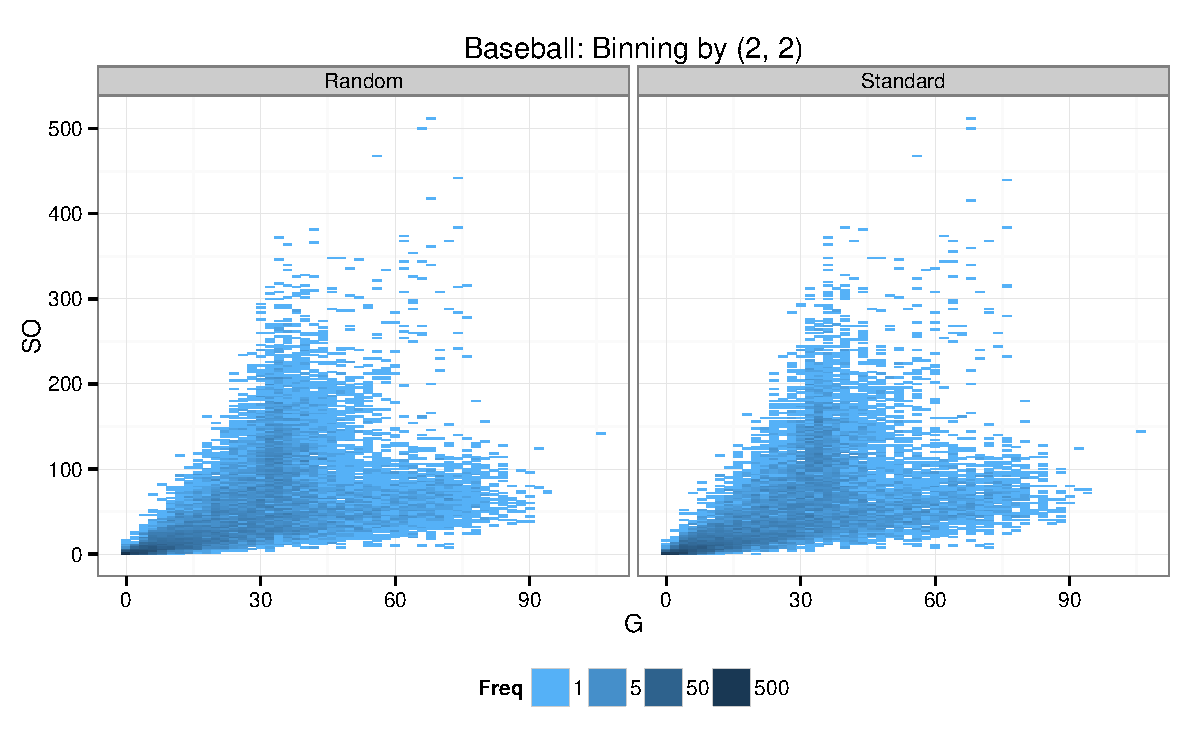
\includegraphics[keepaspectratio=true, width=.9\textwidth]{images/RandomStd22.pdf}
% % }\\
% % \subfloat[(5, 25) tiling of G, SO data]{
% % 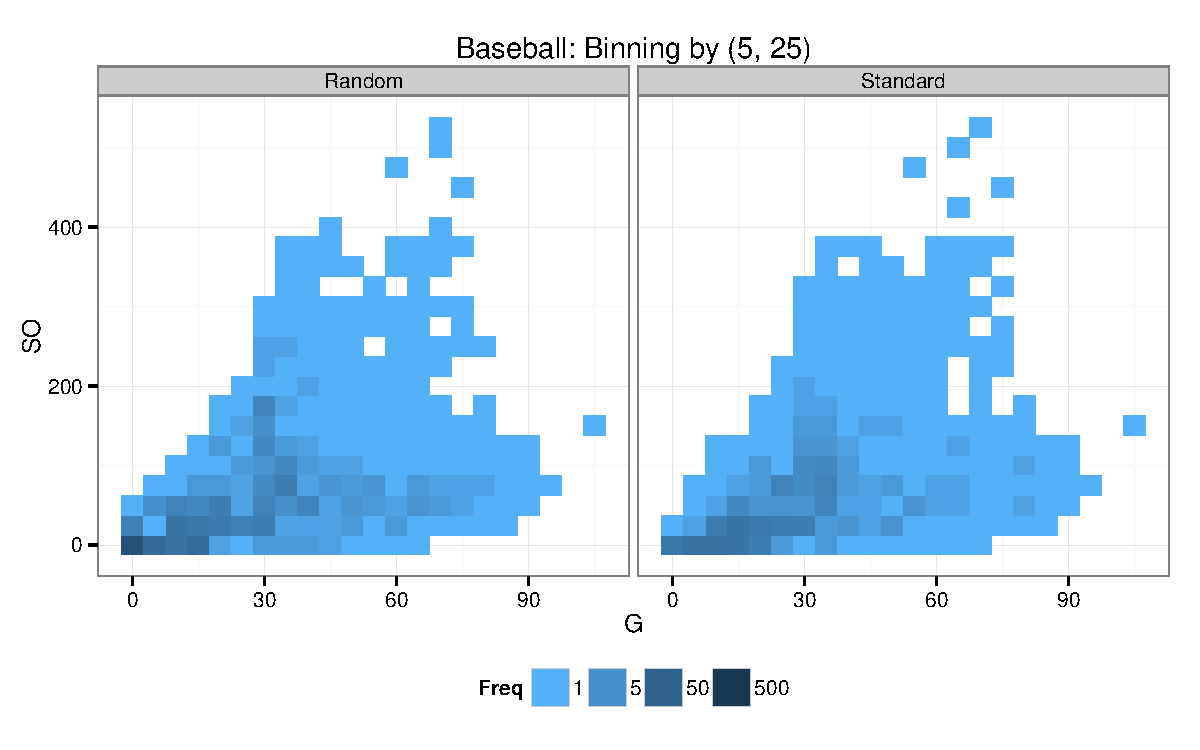
\includegraphics[keepaspectratio=true, width=.9\textwidth]{images/RandomStd525.pdf}
% % }
% % \caption{\label{fig:binning-comparison} Comparison of random and standard binning: standard binning introduces artificial striping when the chosen bin width is not a multiple of the data resolution.}
% % \end{figure}
% % 
% % 
% 
% 
% \subsection{Big Data: Airline Departure Times}
% The Federal Aviation Association (FAA) requires all airlines based in the United States to report   details for every single flight. These are published online by the Bureau of Transportation Services at \url{http://www.transtats.bts.gov/DataIndex.asp}. 
% Every day there are about 16,000 flights across the United States adding up to almost 6 Million flights a year. Scheduled and actual departure times for all flights in 2011 make up --in uncompressed form-- a file of about 450 MB. A comparison of scheduled and actual departure times allows us an investigation of on-time performance of air carriers.
% 
% %We obtained airline scheduled departure times and actual departure times from the Department of Transportation for the year 2011. These times do not include actual departure date, however, so a flight scheduled to leave at 23:00 which is delayed by two hours is recorded as leaving at 01:00. The uncompressed data file is about 450 MB, and consists of two columns of almost six million records. 
% 
% \ktm{Figure~\ref{airline-scatter} shows two plots of the relationship between scheduled versus actual departure times. The plot on the left shows the scatterplot from a sample of one million of those records. Even while using alpha blending this results in a severely over-plotted graph. On the right is a binned scatterplot of the reduced data from standard binning at 1-minute intervals. If the origin is offset by a half minute for both departures and arrivals, this binning does not have any spatial loss, as all observations will be centered within bins. The 1-minute standard binning also reduces the data to 176,384 individual records, less than 3\% of the original data. }
% 
% \begin{figure}[hbtp]\centering
% \subfloat[Million-point sample of Airline Data]{\includegraphics[width=.44\linewidth, keepaspectratio=TRUE]{images/MillionSample.pdf}}\hfill
% %   Swap Back at later date (shrinks size of pdf to managable)
% %\subfloat[Million-point sample of Airline Data. \ktm{This plot is not compiling and needs to be reconstructed (my apologies)}]{\includegraphics[width=.44\linewidth, keepaspectratio=TRUE]{images/RplotFiller.pdf}}\hfil
% \subfloat[Minimal binning of Airline Data]{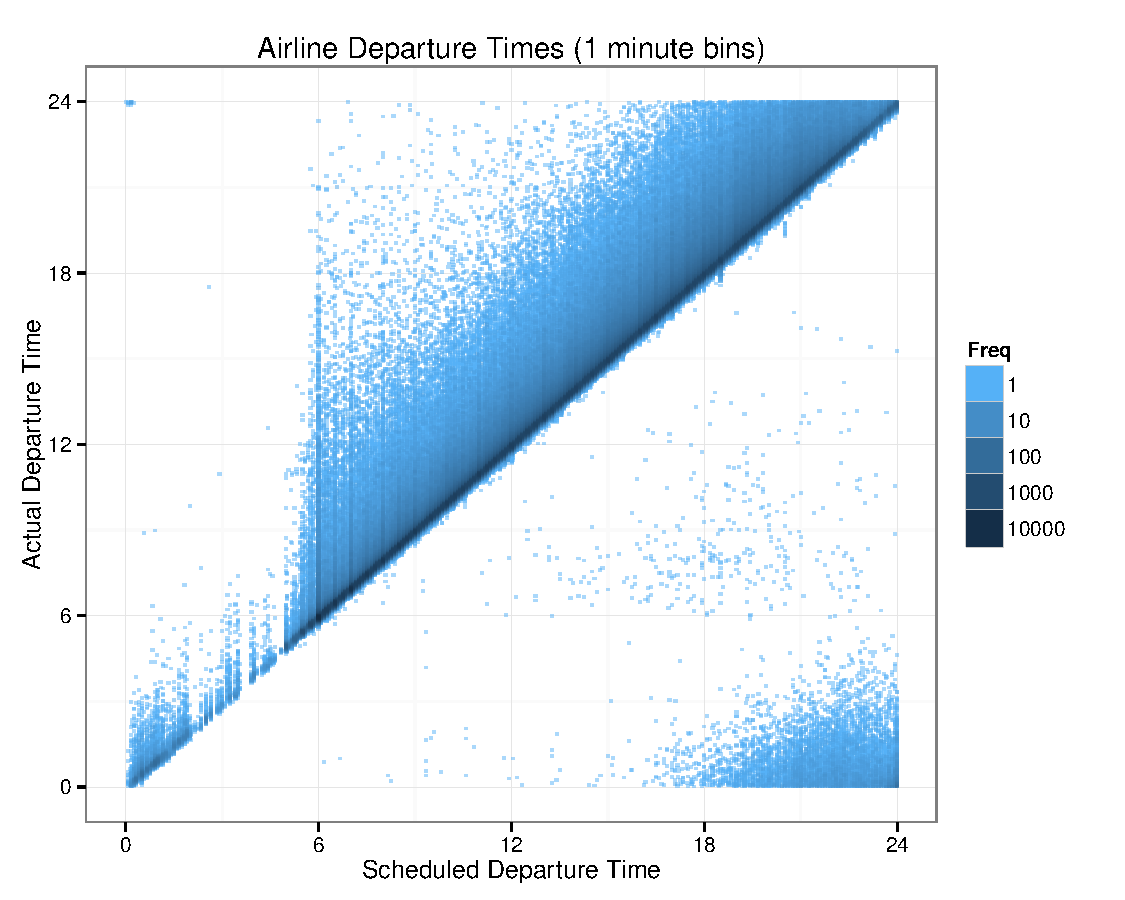
\includegraphics[width=.56\linewidth, keepaspectratio=TRUE]{images/AirlineStdBinning1min.pdf}}
% \caption{\label{airline-scatter}Scheduled and actual departure times of  flights across the United States in 2011. The plot on the left is based on a sample of the data, the plot on the right shows all flights. The large scale distributional patterns are visible in both plots, but the plot on the left misses some of the finer level details in scheduling that is visible in the plot on the right.}
% \end{figure}
% 
% Both plots show the same large scale distributional patterns: scheduled and actual arrival times are highly correlated, recognizable from the conglomeration of points along the line of identity. Scheduled departure times past 6 am in the morning are much more common than earlier flights. It is much more likely for a  flight to be delayed than to leave early, leading to the wash-out effect above the line, that is getting thinner with increasing delays. The range of delays on usual days starts at about one hour at 6 am and increases during the day to about 2 hours. The few number of flights before 6 am are also visible in both plots. The triangle of observations on the bottom right visible in both plots is nothing but an artifact of the data collection consisting of flights that are scheduled before midnight, but are delayed to departures past midnight. The cloud of outliers halfway between the two main structures is potentially interesting, since no immediate explanation comes to mind, and would be worthy of a follow-up investigation.
% 
% What is not apparent in the alpha blended scatterplot, is some fine-level structure that the plot based on all of the data shows. \ktm{Note that because we have bin widths equal to the resolution to which the data is recorded in each dimension, we know that the spatial binning algorithm will not cause any artificial density stripes.} A close inspection of the plot on the right hand side reveals darker colored vertical lines at 30 minute intervals. It is obvious that more flights are scheduled with departures on the hour and at 30 minutes past the hour. 
% 
% \begin{figure}[hbtp]\centering
% 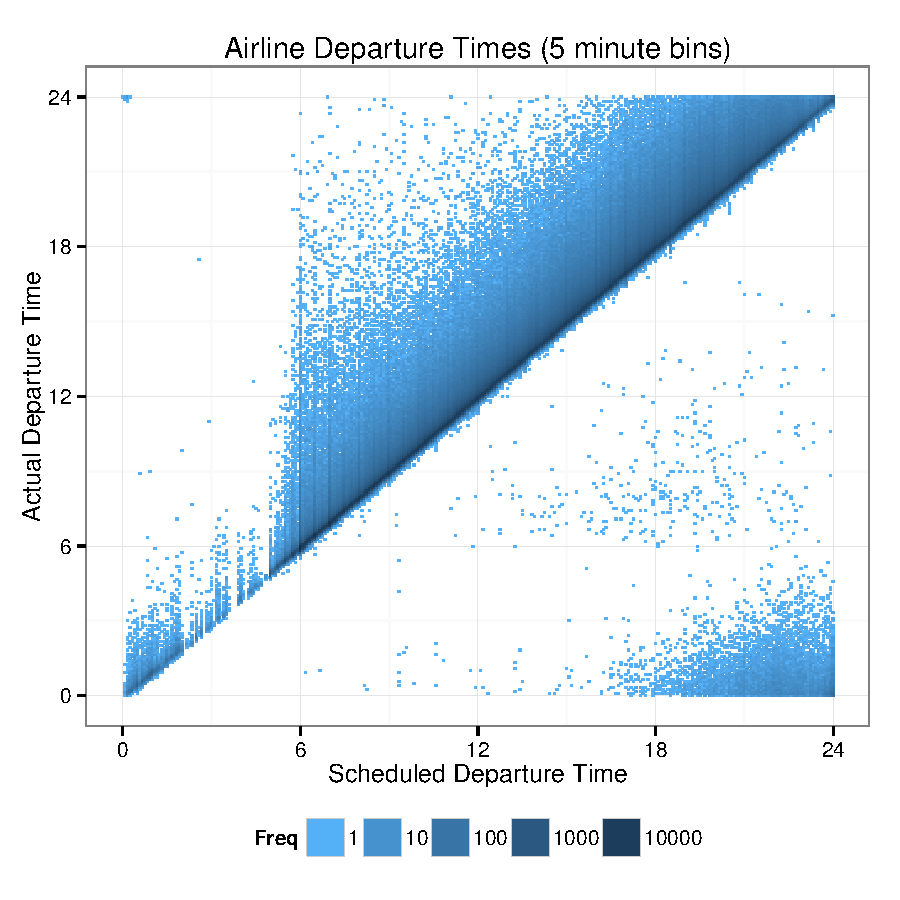
\includegraphics[width=.49\linewidth,keepaspectratio=true]{images/AirlineStdBinning5mins.pdf}
% 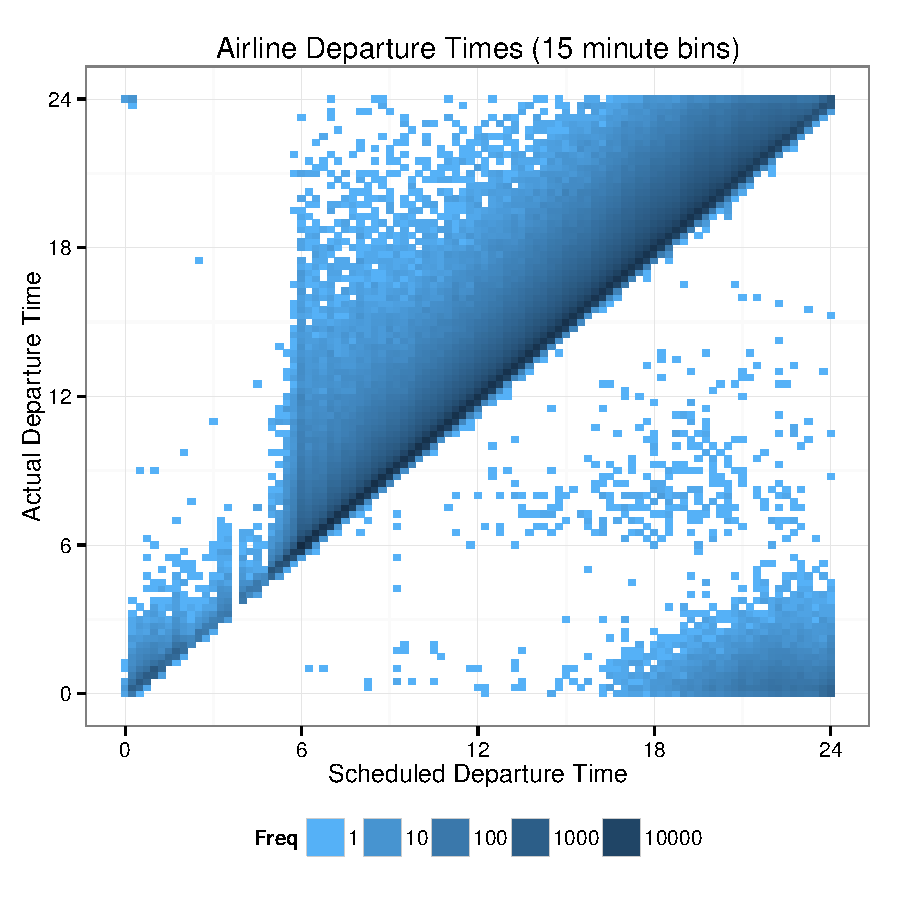
\includegraphics[width=.49\linewidth,keepaspectratio=true]{images/AirlineStdBinning15mins.pdf}
% \caption{5-minute bins produce a higher-level summary of the data than shown in Figure~\ref{airline-scatter}b. 15-minute bins produce an even more coarse summary of the data.}\label{airline5mins-binning}
% \end{figure}
% 
% Figure~\ref{airline5mins-binning} displays the binned scatterplots for the flight departure data with larger bins. Binning data by five-minute intervals produces a more high-level summary of the relationship between actual and scheduled departure time, though it necessarily obscures some of the finer details. In addition, binning data by five minute intervals reduces the size of the data set to a much more manageable 19,787 reduced binned data triples, which can be easily manipulated on probably any modern computer. Binning by 15-minute intervals reduces the data set to a nearly-trivial 3,575 reduced binned data triples, but the graphical summary becomes granular and less appealing at that resolution.
% 
% <<airlinesetup,echo=FALSE, eval=FALSE>>=
% setwd("./data/")
% if (!file.exists("airline.csv.gz")) {
%   # HH: I'm not sure, which files these should be ... 
%   # airline <- do.call("rbind", lapply(list.files(), function(i) read.csv(i)))
%   
%   # write.csv(airline, "airline.csv", row.names=FALSE)
% }
% airline <- read.csv("airline.csv.gz")
% na.departure <- (is.na(airline[,8]) + is.na(airline[,9]))> 0
% airline <- airline[!na.departure,8:9]
% 
% airline$CRS_DEP_TIME <- floor(airline$CRS_DEP_TIME/100)*60 + airline$CRS_DEP_TIME%%100
% airline$DEP_TIME <- floor(airline$DEP_TIME/100)*60 + airline$DEP_TIME%%100
% 
% library(lubridate)
% convert.time <- function(x){
%   floor(x/60) + (x%%60)/60
% }
% 
% library(multicore)
% 
% if (!file.exists("ReducedAirlineData.csv")) {
%   airline.freq <- ddply(airline, .(CRS_DEP_TIME, DEP_TIME), function(i) cbind(unique(i), Freq=nrow(i)))
%   write.csv(airline.freq, "ReducedAirlineData.csv", row.names=FALSE)
% }
% airline.freq <- read.csv("ReducedAirlineData.csv")
% airline.freq.plot <- airline.freq
% airline.freq.plot[,1] <- convert.time(airline.freq.plot[,1])
% airline.freq.plot[,2] <- convert.time(airline.freq.plot[,2])
% airline.freq.plot <- airline.freq.plot[order(airline.freq.plot$Freq),]
% airline.dummy <- airline.freq.plot[1,]
% airline.dummy[1,1] <- NA
% qplot(data=airline.freq.plot, x=CRS_DEP_TIME, y=DEP_TIME, fill=Freq, asp=1, geom="blank", xlab="Scheduled Departure Time", ylab="Actual Departure Time", main="Airline Departure Times (1 minute bins)") + geom_rect(aes(xmin=CRS_DEP_TIME-3/60, xmax=CRS_DEP_TIME+3/60, ymin=DEP_TIME-3/60, ymax=DEP_TIME+3/60, fill=Freq), alpha=I(.5)) + geom_rect(data=airline.dummy, aes(xmin=CRS_DEP_TIME-3/60, xmax=CRS_DEP_TIME+3/60, ymin=DEP_TIME-3/60, ymax=DEP_TIME+3/60, fill=Freq), aes.inherit=FALSE) + theme_bw()+ theme(legend.position="right") +scale_fill_gradientn(colours=c("#56B1F7", "#132B43"), guide="legend", trans="log", breaks=c(1, 10, 100, 1000, 10000))+ scale_x_continuous(breaks=c(0, 6, 12, 18, 24)) + scale_y_continuous(breaks=c(0, 6, 12, 18, 24))
% ggsave("AirlineStdBinning1min.pdf", width=7.5, height=6, dpi=2304)
%     
% 
% library(ggplot2)
% library(dbData)
% air.sample <- airline.freq.plot[sample(1:nrow(airline.freq.plot), 1000000, replace=TRUE, prob=airline.freq.plot$Freq),1:2]
% 
% qplot(data=air.sample, x=CRS_DEP_TIME, y=DEP_TIME, geom="point", alpha=I(.05), xlab="Scheduled Departure Time", ylab="Actual Departure Time", main="Sampled Airline Departure Times") + theme_bw()+ theme(legend.position="right") + scale_x_continuous(breaks=c(0, 6, 12, 18, 24)) + scale_y_continuous(breaks=c(0, 6, 12, 18, 24))
% ggsave("MillionSample.pdf", width=6, height=6, dpi=576)
% 
% if (!file.exists("airlineBin5Std.csv")) {
%   air.binned5 <- binStd(airline.freq, c(5, 5))
%   air.binned5 <- ddply(air.binned5, .(CRS_DEP_TIME, DEP_TIME), function(i) cbind(convert.time(unique(i[,1:2])), Freq=sum(i$Freq)))
%   write.csv(air.binned5, "airlineBin5Std.csv", row.names=FALSE)
% }
% # air.binned5.rdm <- binRdm(cbind(airline, Freq=1), c(5, 5))
% # air.binned5.rdm2 <- ddply(air.binned5.rdm, .(CRS_DEP_TIME, DEP_TIME), function(i) cbind(convert.time(unique(i[,1:2]), Freq=sum(i$Freq)))
% # write.csv(air.binned5.rdm2, "airlineBin5Rdm.csv", row.names=FALSE)
% 
% air.binned5 <- read.csv("airlineBin5Std.csv")
% qplot(data=air.binned5, x=CRS_DEP_TIME, y=DEP_TIME, fill=Freq, asp=1, geom="tile", xlab="Scheduled Departure Time", ylab="Actual Departure Time", main="Airline Departure Times (5 minute bins)") + theme_bw()+ theme(legend.position="bottom") +scale_fill_gradientn(colours=c("#56B1F7", "#132B43"), guide="legend", trans="log", breaks=c(1, 10, 100, 1000, 10000))+ scale_x_continuous(breaks=c(0, 6, 12, 18, 24)) + scale_y_continuous(breaks=c(0, 6, 12, 18, 24))
% ggsave("AirlineStdBinning5mins.pdf", width=6, height=6, dpi=576)
% # 
% # qplot(data=air.binned5.rdm2, x=CRS_DEP_TIME, y=DEP_TIME, fill=Freq, asp=1, geom="tile", xlab="Scheduled Departure Time", ylab="Actual Departure Time", main="Airline Departure Times (5 minute bins)") + theme_bw()+ theme(legend.position="bottom") +scale_fill_gradient(low="#56B4FB", high="#183347", guide="legend", trans="log")
% # ggsave("AirlineRdmBinning5mins.png", binned, width=6, height=6)
% 
% # air.binned <- data.frame(apply(airline, 2, function(i) 15*round(i/15, 0)))
% # air.binned.rdm <- binRdm(airline.freq, c(15, 15))
% # air.binned2 <- ddply(air.binned, .(CRS_DEP_TIME, DEP_TIME), function(i) cbind(unique(i), Freq=sum(i$Freq)))
% # write.csv(air.binned2, "airlineBin15.csv", row.names=FALSE)
% air.binned <- read.csv("airlineBin15.csv")
% air.binned2 <- air.binned
% air.binned2[,1] <- convert.time(air.binned[,1])
% air.binned2[,2] <- convert.time(air.binned[,2])
% air.binned.rdm <- read.csv("airlineBin15Rdm.csv")
% air.binned2.rdm <- air.binned.rdm
% air.binned2.rdm[,1] <- convert.time(air.binned.rdm[,1])
% air.binned2.rdm[,2] <- convert.time(air.binned.rdm[,2])
% 
% # air.binned2.rdm <- ddply(air.binned.rdm, .(CRS_DEP_TIME, DEP_TIME), function(i) cbind(unique(i), Freq=sum(i$Freq)))
% # write.csv(air.binned2.rdm, "airlineBin15Rdm.csv", row.names=FALSE)
% 
% binned <- qplot(data=air.binned2, x=CRS_DEP_TIME, y=DEP_TIME, fill=Freq, asp=1, geom="tile", xlab="Scheduled Departure Time", ylab="Actual Departure Time", main="Airline Departure Times (15 minute bins)") + theme_bw()+ theme(legend.position="bottom") +scale_fill_gradientn(colours=c("#56B1F7", "#132B43"), guide="legend", trans="log", breaks=c(1, 10, 100, 1000, 10000))+ scale_x_continuous(breaks=c(0, 6, 12, 18, 24)) + scale_y_continuous(breaks=c(0, 6, 12, 18, 24))
% ggsave("AirlineStdBinning15mins.pdf", binned, width=6, height=6, dpi=576)
% 
% # binnedRdm <- qplot(data=air.binned2.rdm, x=CRS_DEP_TIME, y=DEP_TIME, fill=Freq, asp=1, geom="tile", xlab="Scheduled Departure Time", ylab="Actual Departure Time", main="Airline Departure Times (15 minute bins)") + theme_bw()+ theme(legend.position="bottom") +scale_fill_gradientn(colours=c("#56B1F7", "#132B43"), guide="legend", trans="log", breaks=c(1, 10, 100, 1000, 10000))+ scale_x_continuous(breaks=c(0, 6, 12, 18, 24)) + scale_y_continuous(breaks=c(0, 6, 12, 18, 24))
% # ggsave("AirlineRdmBinning15mins.png", binnedRdm, width=8, height=8, dpi=600)
% @
% 
% %--------------------------------------------------------------------------------------
% 
% \section{Conclusions and Future Work}
% 
% \ktm{Large Data sets of continuous variables are very difficult to visualize in raw form, due to over-plotting of points. Binning allows for the visualization and manipulation of large data sets, and easily translates into binned scatterplots which are more appropriate for the human visual system. Reducing the data for binned scatterplots has distinct computational and visual advantages, however the aggregation can come at the cost of losing precision in the spatial and frequency information. }
% 
% \ktm{We have presented two algorithms for spatially binning data points; standard and random rectangular binning algorithms. The random binning algorithm displayed strong advantage of avoiding the problem of artificial stripes that occurred when data recorded to a coarse resolution was binned using a bin width that was a non-integer multiple of the resolution. However, standard binning algorithm is superior due to lower spatial loss, and data with coarse resolution ($\alpha_x$ units in the X dimension and $\alpha_y$ units in the Y dimension) can avoid creating artificial stripes if a bin dimensions are integer multiples of $\alpha_x$ and $\alpha_y$.  It was also shown through simulation that for coarse data, a reasonable default for the binning origin is offset to ($\alpha_x/2$,$\alpha_y/2$) because it resulted in minimal or near minimal spatial loss for symmetric data and preformed well even for skewed data.  }
% 
% \ktm{Spatially binning with smaller bin dimensions will lead to lower spatial losses; however, finer binning requires more processing time and does not highlight large scale density structure. It is left to the plot designer to decide how much spatial information they are willing to sacrifice in order to simplify the display of density structure; we do however suggest to err on the side of smaller bins which allow for visualization of finer density structure with lower spatial loss. }
% 
% \ktm{If we elect to use frequency binning to aid the perceptual mapping tile shades to the plot key for frequency, it is recommended to use between four and seven distinct shades. This is done to minimize the frequency loss within the bounds of human perceptual ability to distinguish multiple shades simultaneously. Using quantile frequency binning and log transforming the bin counts prior to standard frequency binning are shown to be reasonable methods -- with slight different interpretability -- for handling situations with heavily skewed bin count distributions. }
% 
% \ktm{Future implementations of software for constructing binned scatterplots would be well served to allow for choices in specification of binning algorithms. The findings of this research provide suggestions for reasonable default settings for binning parameters that maintain of spatial and frequency information and have desirable visual properties. }
% 
% %----------------------------------------------------------------------------
% \newpage
% \begin{appendix}
% \section{Appendix}
% 
% %----------------------------------------------------------------------------
% \subsection{Optimal Offset for Uniform Data Recorded to Resolution $\alpha$}
% \label{proof:offset}
% 
% The following is proof that when univariate data is uniformly distributed at resolution $\alpha$ and standard rectangular binning is used with binwidths that are a scalar multiple of the data resolution (i.e. $\omega = k\alpha$ for some $k \in \{1,2,\dots\})$, then spatial loss is minimized by setting the binning origin to $\alpha/2$ units below the minimum data value; set $\beta = x_{(1)} - \alpha/2$.\\
% 
% \noindent Let $x_1, x_2, \dots, x_k \in \mathbb{R}$ represent the values in a single bin such that $x_{i+1} = x_i + \alpha$ for some constant $\alpha \in \mathbb{R}$. Thus $x_j = x_1 + (j-1)\alpha$.\\ 
% 
% \noindent Suppose then that we bin the data using standard rectangular binning with origin, $\beta = x_1 - \theta$, and binwidth $\omega$; where $\theta$ is the \textit{origin offset} from the data. Thus $b(x_j) = \beta + \omega/2 = (x_1 - \theta) + (k\alpha/2)$\\
% 
% \noindent Spatial Loss, $L^S = \sum_{i=1}^{k} ||x_i-b_(x_i)|| $ is definitionally minimized when $b_(x_i)$ is the \textit{geometric median}. The geometric median for $x_1, \dots, x_k = Q_x(.5) = (x_{\lceil\frac{k+1}{2}\rceil}+x_{\lfloor \frac{k+1}{2}\rfloor})/2$ , where $Q_x(\cdot)$ is the empirical quantile function. \\
% 
% \noindent Thus the optimal offset is the $\theta$ such that\\
% 
% $ b(x_i) = Q_x(.5) $ \\
% $ \Rightarrow (x_1 - \theta) + (k\alpha/2) = (x_{\lceil\frac{k+1}{2}\rceil}+x_{\lfloor \frac{k+1}{2}\rfloor})/2 $ \\
% $ \Rightarrow 2x_1 - 2\theta + k\alpha = (x_1 + (\lceil\frac{k+1}{2}\rceil - 1)\alpha ) + (x_1 + (\lfloor\frac{k+1}{2}\rfloor - 1)\alpha ) $ \\
% $ \Rightarrow -2\theta + k\alpha = (\lceil\frac{k+1}{2}\rceil - 1)\alpha  + (\lfloor\frac{k+1}{2}\rfloor - 1)\alpha  $ \\
% $ \Rightarrow -2\theta + k\alpha = ((k+1) - 2)\alpha  $ \\
% $ \Rightarrow -2\theta = -\alpha $ \\
% $ \Rightarrow \theta = \alpha/2 $ \\
% 
% Thus the optimal offset for reducing spatial loss in this scenario is $\theta = \alpha/2$.  This result holds for data that is symmetrically distributed within the bin since the median will not change.  It extends to multiple contiguous bins with resolution $\alpha$ data that has symmetrically distributed data withing each bin. \\
% 
% If the same conditions are extended to the two dimensional case, then the origin for minimal spatial loss is at $(x_{(1)}-\alpha_x/2, y_{(1)}-\alpha_y/2)$ where $\alpha_x$ and $\alpha_y$  are the data resolution for each dimension, respectively. 
% 
% %----------------------------------------------------------------------------
% % 
% % \subsection{Partition of Spatial Loss}\label{proof:partition}
% % We want to show that spatial loss can be written as a partition of the form 
% % \[L_s(x) = 1/S^2_{\emptyset}\sum_i S^2_i = 1/S^2_{\emptyset}\left[\sum_i L^N_i + \sum_i L^V_i\right]\] 
% % 
% % For that let us consider the values $\{x_{i}: b(x_i) = x^\ast\}$ in a single bin with center $x^\ast$.
% % The numerical center of these points is given as  $1/n \sum x_i = \overline x$.
% % Then the total loss for each element $x_i$ in this bin is:
% % 
% % \begin{align*}
% % S_i^2 = \sum (x_i - x_i^\ast)^2 & = \sum (x_i - \overline x + \overline x - x_i^\ast)^2\\
% % & = \sum(x_i-\overline x)^2 + 2\sum (x_i-\overline x)(\overline x-x_i^\ast) + \sum(\overline x-x_i^\ast)^2\\
% % & = \sum(x_i - \overline x)^2 + 2\sum(0)(\overline x-x_i^\ast) + \sum(\overline x-x_i^\ast)^2\\
% % & = \sum(x_i - \overline x)^2 + \sum(\overline x-x_i^\ast)^2\\
% % & = L^N_i + L^V_i
% % \end{align*}
% % Adding over all elements in the bin and all bins gives the formula above.
% % 
% % \subsection{Constancy of Loss under Binary Splits}\label{proof:constantloss}
% % We want to show that under random binning the loss due to doubling of bin width is deterministic.
% % 
% % Let us consider the contribution $L_i$ of a single point $x_i$ to the loss when starting with the minimal bin width, i.e. each unique point is in a separate bin:
% % doubling the bin width leads to two  scenarios: 
% % a point is either at  the bin center or directly between two bins.
% % In the case that the point is at the bin center, its contribution to the total overall loss is zero,  $L_i = 0$, and the associated probability $p_i = 1$. 
% % 
% % Alternately, when the point is exactly half-way between two bin centers, the point is attributed with probability $p_i = \frac{1}{2}$ to either bin, leading to a loss of $L_i = \frac{1}{2} c_i$ regardless of which bin is assigned. Hence, in this case, loss is also entirely independent of which bin is assigned.
% \end{appendix}

